%Version 3.1 December 2024
% See section 11 of the User Manual for version history
%
%%%%%%%%%%%%%%%%%%%%%%%%%%%%%%%%%%%%%%%%%%%%%%%%%%%%%%%%%%%%%%%%%%%%%%
%%                                                                 %%
%% Please do not use \input{...} to include other tex files.       %%
%% Submit your LaTeX manuscript as one .tex document.              %%
%%                                                                 %%
%% All additional figures and files should be attached             %%
%% separately and not embedded in the \TeX\ document itself.       %%
%%                                                                 %%
%%%%%%%%%%%%%%%%%%%%%%%%%%%%%%%%%%%%%%%%%%%%%%%%%%%%%%%%%%%%%%%%%%%%%

%%\documentclass[referee,sn-basic]{sn-jnl}% referee option is meant for double line spacing

%%=======================================================%%
%% to print line numbers in the margin use lineno option %%
%%=======================================================%%

%%\documentclass[lineno,pdflatex,sn-basic]{sn-jnl}% Basic Springer Nature Reference Style/Chemistry Reference Style

%%=========================================================================================%%
%% the documentclass is set to pdflatex as default. You can delete it if not appropriate.  %%
%%=========================================================================================%%

%%\documentclass[sn-basic]{sn-jnl}% Basic Springer Nature Reference Style/Chemistry Reference Style

%%Note: the following reference styles support Namedate and Numbered referencing. By default the style follows the most common style. To switch between the options you can add or remove “Numbered” in the optional parenthesis. 
%%The option is available for: sn-basic.bst, sn-chicago.bst%  
 
%%\documentclass[pdflatex,sn-nature]{sn-jnl}% Style for submissions to Nature Portfolio journals
%%\documentclass[pdflatex,sn-basic]{sn-jnl}% Basic Springer Nature Reference Style/Chemistry Reference Style
\documentclass[pdflatex,sn-mathphys-num]{sn-jnl}% Math and Physical Sciences Numbered Reference Style
%%\documentclass[pdflatex,sn-mathphys-ay]{sn-jnl}% Math and Physical Sciences Author Year Reference Style
%%\documentclass[pdflatex,sn-aps]{sn-jnl}% American Physical Society (APS) Reference Style
%%\documentclass[pdflatex,sn-vancouver-num]{sn-jnl}% Vancouver Numbered Reference Style
%%\documentclass[pdflatex,sn-vancouver-ay]{sn-jnl}% Vancouver Author Year Reference Style
%%\documentclass[pdflatex,sn-apa]{sn-jnl}% APA Reference Style
%%\documentclass[pdflatex,sn-chicago]{sn-jnl}% Chicago-based Humanities Reference Style

%%%% Standard Packages
%%<additional latex packages if required can be included here>

\usepackage{graphicx}%
\usepackage{multirow}%
\usepackage{amsmath,amssymb,amsfonts}%
\usepackage{amsthm}%
\usepackage{mathrsfs}%
\usepackage[title]{appendix}%
\usepackage{xcolor}%
\usepackage{textcomp}%
\usepackage{manyfoot}%
\usepackage{booktabs}%
\usepackage{subcaption}%
\usepackage{algorithm}%
\usepackage{algorithmicx}%
\usepackage{algpseudocode}%
\usepackage{listings}%
\usepackage{longtable}
\usepackage{soul}
\usepackage{bm}
\usepackage{dblfloatfix}%
\setcounter{dbltopnumber}{4}%
\renewcommand{\dbltopfraction}{0.99}%
\usepackage{placeins}%
\usepackage{afterpage}%
\DeclareUnicodeCharacter{02BC}{'}
%%%%

%%%%%=============================================================================%%%%
%%%%  Remarks: This template is provided to aid authors with the preparation
%%%%  of original research articles intended for submission to journals published 
%%%%  by Springer Nature. The guidance has been prepared in partnership with 
%%%%  production teams to conform to Springer Nature technical requirements. 
%%%%  Editorial and presentation requirements differ among journal portfolios and 
%%%%  research disciplines. You may find sections in this template are irrelevant 
%%%%  to your work and are empowered to omit any such section if allowed by the 
%%%%  journal you intend to submit to. The submission guidelines and policies 
%%%%  of the journal take precedence. A detailed User Manual is available in the 
%%%%  template package for technical guidance.
%%%%%=============================================================================%%%%

%% as per the requirement new theorem styles can be included as shown below
\theoremstyle{thmstyleone}%
\newtheorem{theorem}{Theorem}%  meant for continuous numbers
%%\newtheorem{theorem}{Theorem}[section]% meant for sectionwise numbers
%% optional argument [theorem] produces theorem numbering sequence instead of independent numbers for Proposition
\newtheorem{proposition}[theorem]{Proposition}% 
%%\newtheorem{proposition}{Proposition}% to get separate numbers for theorem and proposition etc.

\theoremstyle{thmstyletwo}%
\newtheorem{example}{Example}%
\newtheorem{remark}{Remark}%

\theoremstyle{thmstylethree}%
\newtheorem{definition}{Definition}%

\newcommand{\danique}[1]{\textcolor{magenta}{#1}}
\newcommand{\ana}[1]{\textcolor{blue}{#1}}
\newcommand{\blue}[1]{\textcolor{blue}{#1}}
\newcommand{\set}[1]{\mathcal{#1}}


\raggedbottom
%%\unnumbered% uncomment this for unnumbered level heads

\begin{document}
% Complete-coverage California wildfires detection in minutes with optimized drone network
\title[Minutes Matter: Rapid Wildfire Detection Through Sensor Placement and Drone Routing]{Minutes Matter: Rapid Wildfire Detection Through Sensor Placement and Drone Routing}
% \title[Guiding Policy Decisions for Early Wildfire Detection: Optimized Drone and Sensor Deployment in California]{Guiding Policy Decisions for Early Wildfire Detection: Optimized Drone and Sensor Deployment in California}

%%=============================================================%%
%% GivenName	-> \fnm{Joergen W.}
%% Particle	-> \spfx{van der} -> surname prefix
%% FamilyName	-> \sur{Ploeg}
%% Suffix	-> \sfx{IV}
%% \author*[1,2]{\fnm{Joergen W.} \spfx{van der} \sur{Ploeg} 
%%  \sfx{IV}}\email{iauthor@gmail.com}
%%=============================================================%%

\author*[1]{\fnm{Romain} \sur{Puech}}\email{puech@mit.edu}

\author[2]{\fnm{Danique} \sur{de Moor}}\email{demoor@mit.edu}
% \equalcont{These authors contributed equally to this work.}

\author[3]{\fnm{Ana} \sur{Trišović}}\email{ana\_tris@mit.edu}
% \equalcont{These authors contributed equally to this work.}

% \author[1]{\fnm{Joseph} \sur{Ye}}\email{justdoye@mit.edu}

\author[2]{\fnm{Dimitris} \sur{Bertsimas}}\email{dbertsim@mit.edu}

\affil*[1]{\orgdiv{Operations Research Center}, \orgname{Massachusetts Institute of Technology}, \orgaddress{\street{77 Massachusetts Avenue}, \city{Cambridge}, \postcode{02139}, \state{MA}, \country{USA}}}

\affil[2]{\orgdiv{Sloan School of Management}, \orgname{Massachusetts Institute of Technology}, \orgaddress{\street{77 Massachusetts Avenue}, \city{Cambridge}, \postcode{20139}, \state{MA}, \country{USA}}}

\affil[3]{\orgdiv{Computer Science \& Artificial Intelligence Laboratory}, \orgname{Massachusetts Institute of Technology}, \orgaddress{\street{77 Massachusetts Avenue}, \city{Cambridge}, \postcode{20139}, \state{MA}, \country{USA}}}

%%==================================%%
%% Sample for unstructured abstract %%
%%==================================%%

% \abstract{Early wildfire detection is critical to prevent small ignitions from escalating into large-scale disasters, yet current monitoring systems lack a quantitative framework for allocating detection infrastructure at scale. Here we develop an integrated optimization framework that jointly determines the placement of monitoring infrastructure and the routing of autonomous drones for proactive wildfire detection. Using California as a case study, we show that rapid, near-complete detection is achievable under realistic operational and budget constraints. An optimized drone-based monitoring network operating at a \$100 million budget detects 96\% of benchmark wildfire ignitions, \danique{with a mean detection time of approximately 17 minutes and a maximum of two hours}. Detection performance improves nonlinearly with investment, with rapid gains as infrastructure expands to bring previously unreachable areas within monitoring range, followed by diminishing returns once most fires occur within the system’s operational reach. Under current cost assumptions, drone-based monitoring economically outperforms ground sensors, with a cost sensitivity analysis showing how the optimal mix of static sensors and drones shifts with relative unit costs. Our results reveal that detection performance is primarily governed by the spatial reach of the monitoring network, while routing strategies mainly influence detection speed. This framework provides quantitative guidance for designing cost-effective wildfire monitoring systems and is readily applicable to other regions.
\abstract{Early wildfire detection is critical to prevent small ignitions from escalating into large-scale disasters, yet current monitoring systems lack a quantitative framework for allocating detection infrastructure at scale. We develop an integrated optimization framework that jointly determines the placement of monitoring infrastructure and the routing of drones for proactive wildfire detection. Using California as a case study, we show that near-complete detection is achievable under realistic operational and budget constraints at a cost below 0.1\% of recent wildfire losses \ana{which exceeded XXX in California last year}. An optimized drone-based network operating at a \$100 million budget detects 97.3\% of historical wildfire ignitions, with 74\% of detections occurring within the first hour of ignition. Detection performance is threshold-driven, with rapid gains as infrastructure expands to cover previously unreachable areas, followed by diminishing returns once most fires lie within the system's reach. We find that drone-based monitoring is more cost-effective than static ground sensors, with sensitivity analysis showing how the optimal mix depends on relative costs. Overall, detection performance is governed by spatial coverage, while drone routing choice primarily affects detection speed. 
}

% \abstract{\ana{California spent \$440M on wildfire prevention in 2024 but lacks a quantitative framework for allocating detection infrastructure \danique{Is this the case? Alertcalifornia has a network right}. Here we show that a \$100M optimized drone-sensor network would detect 96\% of evaluated benchmark 2021 wildfire ignitions (94 of 98 scenarios) within 17 minutes on average.} Early detection is critical for preventing small ignitions in California from escalating into destructive wildfires, especially as climate change accelerates fire spread. Satellite systems provide broad coverage but often miss early-stage fires due to limited revisit times and resolution, whereas drones can deliver rapid, flexible, and terrain-independent monitoring. To guide policy makers in planning effective systems, we quantify (i) the detection performance achievable within a {\color{orange} 6–24} hour window, (ii) the required mix of drones, charging stations, and ground sensors, (iii) the optimal spatial placement of these resources across California, and (iv) how optimized fleets behave operationally. Our integrated optimization model incorporates the state’s existing ground-sensor network and reveals a strong budget–detection frontier, with detection improving from {\color{orange}55$\%$} under low budgets to over {\color{orange} 90$\%$} with larger investments. Spatial deployment and visitation patterns highlight where infrastructure yields the largest marginal benefit. The framework provides clear, quantitative guidance for wildfire-monitoring investments and resource allocation, to strengthen early detection and reduce suppression costs. \danique{Maximizing coverage versus minimizing detection time. Detect 96 percent of fires in 17 minutes with budget of 100 million}.
% % Optimized spatial deployments and visitation patterns highlight how drone fleets dynamically concentrate patrols in high-risk regions, providing clear, quantitative guidance for wildfire-monitoring investments.
% Spatial deployment and visitation patterns highlight where infrastructure yields the largest marginal benefit. The framework provides policy makers with actionable guidance on prioritizing wildfire-monitoring resources to strengthen early detection and reduce suppression costs.}

%%================================%%
%% Sample for structured abstract %%
%%================================%%

% \abstract{\textbf{Purpose:} The abstract serves both as a general introduction to the topic and as a brief, non-technical summary of the main results and their implications. The abstract must not include subheadings (unless expressly permitted in the journal's Instructions to Authors), equations or citations. As a guide the abstract should not exceed 200 words. Most journals do not set a hard limit however authors are advised to check the author instructions for the journal they are submitting to.
% 
% \textbf{Methods:} The abstract serves both as a general introduction to the topic and as a brief, non-technical summary of the main results and their implications. The abstract must not include subheadings (unless expressly permitted in the journal's Instructions to Authors), equations or citations. As a guide the abstract should not exceed 200 words. Most journals do not set a hard limit however authors are advised to check the author instructions for the journal they are submitting to.
% 
% \textbf{Results:} The abstract serves both as a general introduction to the topic and as a brief, non-technical summary of the main results and their implications. The abstract must not include subheadings (unless expressly permitted in the journal's Instructions to Authors), equations or citations. As a guide the abstract should not exceed 200 words. Most journals do not set a hard limit however authors are advised to check the author instructions for the journal they are submitting to.
% 
% \textbf{Conclusion:} The abstract serves both as a general introduction to the topic and as a brief, non-technical summary of the main results and their implications. The abstract must not include subheadings (unless expressly permitted in the journal's Instructions to Authors), equations or citations. As a guide the abstract should not exceed 200 words. Most journals do not set a hard limit however authors are advised to check the author instructions for the journal they are submitting to.}

% \keywords{Early wildfire detection, resource allocation, , Keyword4}

%%\pacs[JEL Classification]{D8, H51}

%%\pacs[MSC Classification]{35A01, 65L10, 65L12, 65L20, 65L70}

\maketitle

% \tableofcontents


% \section*{Literature review}
% Recent work integrates UAVs with air-quality sensors to detect early-stage wildfires through pollutant signatures, enabling detection prior to visible ignition. However, these approaches focus on sensing and energy efficiency, rather than system-level coordination and routing strategies. \cite{rjoub2023uas_wildfire_detection}

% Recent work employs deep reinforcement learning to coordinate multiple UAVs for real-time tracking of wildfire evolution under uncertainty. However, these approaches assume the fire is already detected and do not address early detection or system-level design \cite{julian2019distributed_wildfire}




\section*{Introduction}
\danique{700-1000 words}\\
% Wildfires and associated forest loss have intensified in recent years~\citep{curtis2018classifying, tyukavina2022global, hu2025coexposure, science25}. Nearly half of the 200 most damaging wildfire disasters recorded between 1980 and 2023 occurred in the last decade, highlighting a recent surge in extreme fire events~\citep{science25}. The consequences can be devastating for both human communities and natural ecosystems. For example, the 2019–2020 ``Black Summer'' fires in Australia burned nearly 19 million hectares, caused 33 direct fatalities, and destroyed more than 3,000 homes~\citep{nhra2023blacksummer}. The fires also affected an estimated three billion animals and released hundreds of millions of tonnes of carbon dioxide into the atmosphere, comparable to Australia's annual fossil fuel emissions~\citep{ward2020biodiversity,van2021australian}. In the United States, the 2018 Camp Fire in California caused 85 fatalities and economic losses exceeding \$16 billion~\citep{hamideh2022wildfire}. More recently, the January 2025 Los Angeles wildfires caused 31 fatalities, destroyed more than 16,000 structures, and generated economic losses exceeding \$150 billion, making them among the costliest natural disasters in U.S. history~\citep{calfire2025deadliest,laedc2025wildfires}. These disasters coincide with increasingly extreme fire weather linked to climate change and the expansion of human settlements in the wildland–urban interface, which together amplify wildfire risk~\citep{science25}.
% Wildfires and associated forest loss have intensified in recent years~\citep{curtis2018classifying, tyukavina2022global, hu2025coexposure}. In 2025 alone, wildfires burned approximately 390 million hectares of land worldwide~\citep{GAR2025}. Wildfires rank among the most economically destructive natural hazards, with global losses estimated at \$106 billion between 2014 and 2023~\citep{GAR2025}. A substantial share of these losses occurs in the United States, which accounts for nine of the ten most expensive wildfire disasters recorded since 1970~\citep{GAR2025}. However, economic losses likely underestimate the true societal impact of wildfire events, as ecological degradation, biodiversity loss, and human displacement are often poorly captured in financial assessments~\citep{GAR2025}.

\noindent Wildfires and associated forest loss have intensified in recent years, causing widespread ecological and economic damage~\citep{curtis2018classifying, tyukavina2022global, hu2025coexposure}. In 2025 alone, wildfires burned approximately 390 million hectares of land worldwide~\citep{GAR2025}. Over the past decade, global wildfire losses have exceeded \$100 billion, with a disproportionate share occurring in the United States~\citep{GAR2025}, especially California. These figures likely underestimate the true societal impact, as ecological degradation, biodiversity loss, and human displacement are often not fully captured in financial assessments.

% Recent wildfire disasters illustrate the magnitude of these impacts. Nearly half of the 200 most damaging wildfire disasters recorded between 1980 and 2023 occurred in the last decade, highlighting a recent surge in extreme fire events~\citep{science25}. The 2019–2020 ``Black Summer'' fires in Australia burned nearly 19 million hectares, caused 33 direct fatalities, destroyed more than 3,000 homes~\citep{nhra2023blacksummer}, affected an estimated three billion animals and released hundreds of millions of tonnes of carbon dioxide into the atmosphere~\citep{ward2020biodiversity,van2021australian}. In the United States, the 2018 Camp Fire in California caused 85 fatalities and economic losses exceeding \$16 billion~\citep{hamideh2022wildfire}. More recently, the January 2025 Los Angeles wildfires caused 31 fatalities, destroyed more than 16,000 structures, and generated economic losses exceeding \$150 billion~\citep{calfire2025deadliest,laedc2025wildfires}, considering also indirect impacts. These disasters coincide with increasingly extreme fire weather linked to climate change and the expansion of human settlements in the wildland–urban interface, which together amplify wildfire risk~\citep{science25}. Looking forward, empirical models project that even under ~1.5 °C warming, extra-tropical regions will experience larger and more intense wildfires, and current suppression policies are projected to fail across much of the world~\cite{haas2026wildfires}.

Recent wildfire disasters highlight the increasing severity of these events. Nearly half of the 200 most damaging wildfires since 1980 have occurred in the past decade~\citep{science25}. The 2019–2020 ``Black Summer'' fires in Australia burned nearly 19 million hectares and affected an estimated three billion animals~\citep{nhra2023blacksummer,ward2020biodiversity}. In the United States, the 2018 Camp Fire caused 85 fatalities and more than \$16 billion in losses~\citep{hamideh2022wildfire}, while the January 2025 Los Angeles wildfires resulted in over \$150 billion in damages~\citep{calfire2025deadliest,laedc2025wildfires}. These disasters coincide with increasingly extreme fire weather linked to climate change and the expansion of human settlements in the wildland–urban interface, which together amplify wildfire risk~\citep{science25}. Looking forward, empirical models project that even under ~1.5 °C warming, extra-tropical regions will experience larger and more intense wildfires, and current suppression policies are projected to fail across much of the world~\cite{haas2026wildfires}.

% Effective monitoring and early detection are therefore crucial to ensure that fires remain manageable and to minimize their societal and environmental impacts. Traditional detection approaches rely primarily on ground sensor networks and satellites, but both have important limitations. Ground sensors offer limited spatial visibility and can be costly to deploy and maintain at scale, while satellites often lack the spatial and temporal resolution required for timely detection of rapidly evolving fires~\citep{WildfireDetectionBouguettaya}. 

Effective monitoring and early detection are therefore critical to limit wildfire spread and reduce associated losses. Wildfire mitigation investments are widely recognized to yield substantial economic benefits, with estimates suggesting that every \$1 spent on mitigation can save approximately \$3 in recovery costs~\citep{next10_rebuilding_resilient_2021}. For example, California’s recent allocation of \$2.5 billion for post-fire recovery implies that mitigation investments on the order of \$0.8–0.9 billion could achieve comparable avoided losses. Traditional detection approaches rely primarily on ground sensor networks and satellites, but both have important limitations. Ground sensors offer limited spatial visibility and can be costly to deploy and maintain at scale, while satellites often lack the spatial and temporal resolution required for timely detection of rapidly evolving fires~\citep{WildfireDetectionBouguettaya}.

Unmanned aerial vehicles (UAVs), or drones, offer a promising alternative for large-scale wildfire monitoring. Their ability to survey remote areas with high spatial and temporal resolution, combined with relatively low operational costs, makes them well suited for early fire detection~\citep{WildfireDetectionBouguettaya,WildfireDetectionDLGhali22}. Advances in onboard sensing and machine learning have further improved detection capabilities, enabling drones to identify smoke or flames in real time~\citep{WildfireDetectionDLKim,WildfireDetectionDLKumar24,WildfireDetectionDLYang}. However, most existing work assumes pre-defined flight paths, leaving the critical problem of how to optimally route drones to discover unknown fires largely unexplored.

% Unmanned aerial vehicles (UAVs), or drones, are increasingly recognized as a promising technology for wildfire monitoring. Their ability to survey large and remote areas with high spatial and temporal resolution, combined with relatively low operational costs, makes them well suited for early fire detection~\citep{WildfireDetectionBouguettaya,WildfireDetectionDLGhali22}. Advances in onboard sensing and deep learning have further improved aerial wildfire detection, enabling drones to reliably identify smoke or flames in real time~\citep{WildfireDetectionDLGhali22,WildfireDetectionDLKim,WildfireDetectionDLKumar24,WildfireDetectionDLYandouzi22,WildfireDetectionDLYang}. However, most existing studies assume that drones follow pre-defined flight paths, leaving the critical question of how to actively plan drone routes to maximize early fire discovery largely unexplored.

There are many approaches for generic UAV routing (see e.g., \cite{s23031463, drones9040263, s23031463}). Existing research on drone routing \blue{in wildfire contexts} largely focuses on post-detection monitoring and response, where fire locations are known and the objective is to track fire perimeters or support suppression efforts~\citep{WildfireMonitoringBailonruiz22,DroneroutingPostGhamry17}. In contrast, proactive wildfire detection requires drones to search for unknown ignition events across large and heterogeneous landscapes. Prior work has explored optimization-based, heuristic, \blue{and decentralized swarm-based approaches} for wildfire monitoring~\citep{DroneroutingDeLaFuente,fire7070254,DroneroutingXu, Tzoumas2023, DroneroutingJemmali}, 
but often neglects key operational constraints such as limited battery capacity, recharging requirements, and the need to adapt surveillance to evolving wildfire risk. \blue{In addition, learning-based approaches, including reinforcement learning and neural network-based methods, are promising~\cite{Demir2024, Pordal2025}, but are primarily evaluated in simulation and often require recomputation or retraining when the environment changes. 
Prior work has also considered integrated optimization of ground infrastructure and UAV inspection routing under energy constraints~\citep{Liu2025}, but the UAV coordination is limited to partitioning predefined coverage paths, rather than determining routes as part of the optimization problem. } As a result, the integration of intelligent routing with sensing and infrastructure design remains limited.

% Existing research on drone routing largely focuses on post-detection monitoring and response, where the fire location is already known and the objective is to track fire perimeters, coordinate suppression activities, or support firefighter operations (see, e.g.,~\cite{FirefightingPSO,WildfireMonitoringBailonruiz22,DroneroutingPostGhamry17}). In contrast, proactive wildfire detection, where drones must search for unknown fires across large landscapes, has received comparatively limited attention. This gap is particularly critical given the large economic benefits of early wildfire mitigation, with estimates suggesting that every \$1 spent on mitigation can save approximately \$3 in recovery costs~\citep{next10_rebuilding_resilient_2021}. For example, California’s recent allocation of \$2.5 billion for post-fire recovery in the Los Angeles region implies that a mitigation investment on the order of \$0.8–0.9 billion could achieve comparable avoided recovery expenditures.

% Prior work on wildfire monitoring has explored mixed-integer optimization models, probabilistic path planning approaches, and clustering-based patrol strategies~\citep{DroneroutingDeLaFuente,fire7070254,DroneroutingXu}. However, many of these approaches neglect critical operational constraints such as limited battery capacity, recharging requirements, and the need to adapt monitoring strategies to evolving wildfire risk. As a result, the integration of intelligent routing strategies with sensing technologies remains limited. \danique{Update (especially reinforcement learning efforts)!}

In this work, we develop an integrated framework for proactive wildfire detection that jointly optimizes infrastructure deployment and drone routing under realistic operational constraints. We evaluate the framework using California as a case study due to the availability of detailed wildfire and environmental data, while emphasizing that the approach is general and applicable to other regions.

% Effective early wildfire detection requires combining intelligent drone routing with reliable sensing across different monitoring systems. In practice, this means coordinating mobile drones with stationary ground sensors while adapting surveillance routes to changing wildfire risk. These operations must also account for practical constraints such as limited battery capacity, communication range, and the need for timely data transmission. These challenges raise several key questions: How should drones be routed to maximize early fire detection? How should monitoring strategies adapt as wildfire risk evolves? And how should drones and sensors be deployed when resources are limited?

Our results show that rapid, near-complete wildfire detection is achievable within hours under realistic operational and budget constraints. An optimized drone-based monitoring network operating at a \$100 million budget detects 97.3\% of benchmark wildfire ignitions, with 74\% of detections occurring within the first hour of ignition and all but one detected fire identified within four hours.
% Detection performance improves nonlinearly with investment, with rapid gains as infrastructure expands to bring previously unreachable areas within monitoring range, followed by diminishing returns once most fires occur within the system’s operational reach. 
Under current cost assumptions, drone-based monitoring substantially outperforms ground sensors, providing greater spatial coverage per unit cost.

Importantly, these results reveal a fundamental system insight: wildfire detection performance is primarily determined by the spatial reach of the monitoring network, while routing strategies mainly influence detection speed once fires fall within range. This distinction highlights the central role of infrastructure design in enabling effective large-scale wildfire monitoring.

% We develop an integrated decision framework for proactive wildfire detection and evaluate this framework using California as a case study due to its rich wildfire and environmental data, while noting that the approach is general and applicable to other regions. Our results show that near-complete early wildfire detection across California is achievable within minutes under realistic operational and budget constraints. Specifically, an optimized drone-based monitoring network operating at a \$100 million budget detects 96\% of benchmark wildfire ignitions within six hours, with a mean detection time of approximately 17 minutes. Detection performance improves nonlinearly with investment, with rapid gains as infrastructure expands to bring previously unreachable areas within monitoring range, followed by diminishing returns once most fires occur within the system’s operational reach. Under current cost assumptions, drone-based monitoring dominates ground sensors, as mobile aerial surveillance provides substantially greater spatial coverage per unit cost. Static sensors only become relevant at high budget levels, where they are used to close small residual gaps in coverage.

% These results reveal that wildfire detection performance is primarily determined by the spatial reach of the monitoring network, while routing strategies mainly influence detection speed once fires are within range.

Our contributions include: (1) a systematic characterization of the budget-detection-speed trade-off for wildfire detection at the scale of a U.S. state; (2) evidence that drone-based monitoring economically dominates ground sensor networks under current cost assumptions, together with a cost sensitivity analysis of ground-sensor unit pricing that maps when static sensors, aerial infrastructure, or both appear in the optimal mix; (3) the finding that over 97\% of California's 2021--2024 wildfire ignitions can be detected within four hours, with 74\% identified within the first hour, using less than 25\% of the current CAL FIRE prevention budget; and (4) the development of an open, scalable optimization framework and benchmark for wildfire monitoring that can be applied to other regions.

% Our contributions include:
% (1) A systematic characterization of the budget–detection-time trade-off for wildfire detection at the scale of a U.S. state;
% (2) Evidence that drone-based monitoring economically dominates ground sensor networks under current cost assumptions, \danique{supported by a break-even analysis identifying when this advantage may reverse};
% (3) The finding that over 90\% of California’s 2021 wildfire ignitions can be detected within two hours using less than 25\% of the current CAL FIRE prevention budget; and
% (4) the development of an open, scalable optimization framework and benchmark for wildfire monitoring that can be applied to other regions.

% \st{we develop an integrated decision framework for proactive wildfire detection that jointly optimizes the deployment of ground sensors, the placement of drone charging stations, and the routing of multiple drones under realistic operational constraints such as limited battery capacity and communication range. The framework enables coordinated monitoring of high-risk landscapes by combining risk-aware surveillance strategies with heterogeneous sensing systems. To support the development and evaluation of such monitoring systems, we provide an open-source experimental platform that integrates wildfire risk data, drone specifications, and operational constraints within a unified environment. We evaluate the framework using historical wildfire ignition records from California, one of the most wildfire-prone regions globally, enabling realistic assessment of early detection performance based on where fires actually occur.}

% \section{Observations}
% \begin{itemize}
%     \item Figures drive the paper
%     \item Nature prefers results-driven storytelling.
%     \item Organization: introduction (problem, gap, literature survey brief, contribution/solution, overview of findings), results (dataset description, system architecture, detection performance improvements, infrastructure design results, policy implications), discussion (interpretation of results, policy implications, limitations, future research), method (optimization models, algorithms, data processing, simulation setup etc).
% \end{itemize}

\newpage




%%%%%%%%%%%%%%%%%%%%%%%


\section*{Results}
\danique{around 2200 words}
\subsection*{Wildfire monitoring framework}

\begin{figure*}[!b]
    \centering

    % % First row
    % \begin{subfigure}[t]{0.55\textwidth}
    %     \centering
        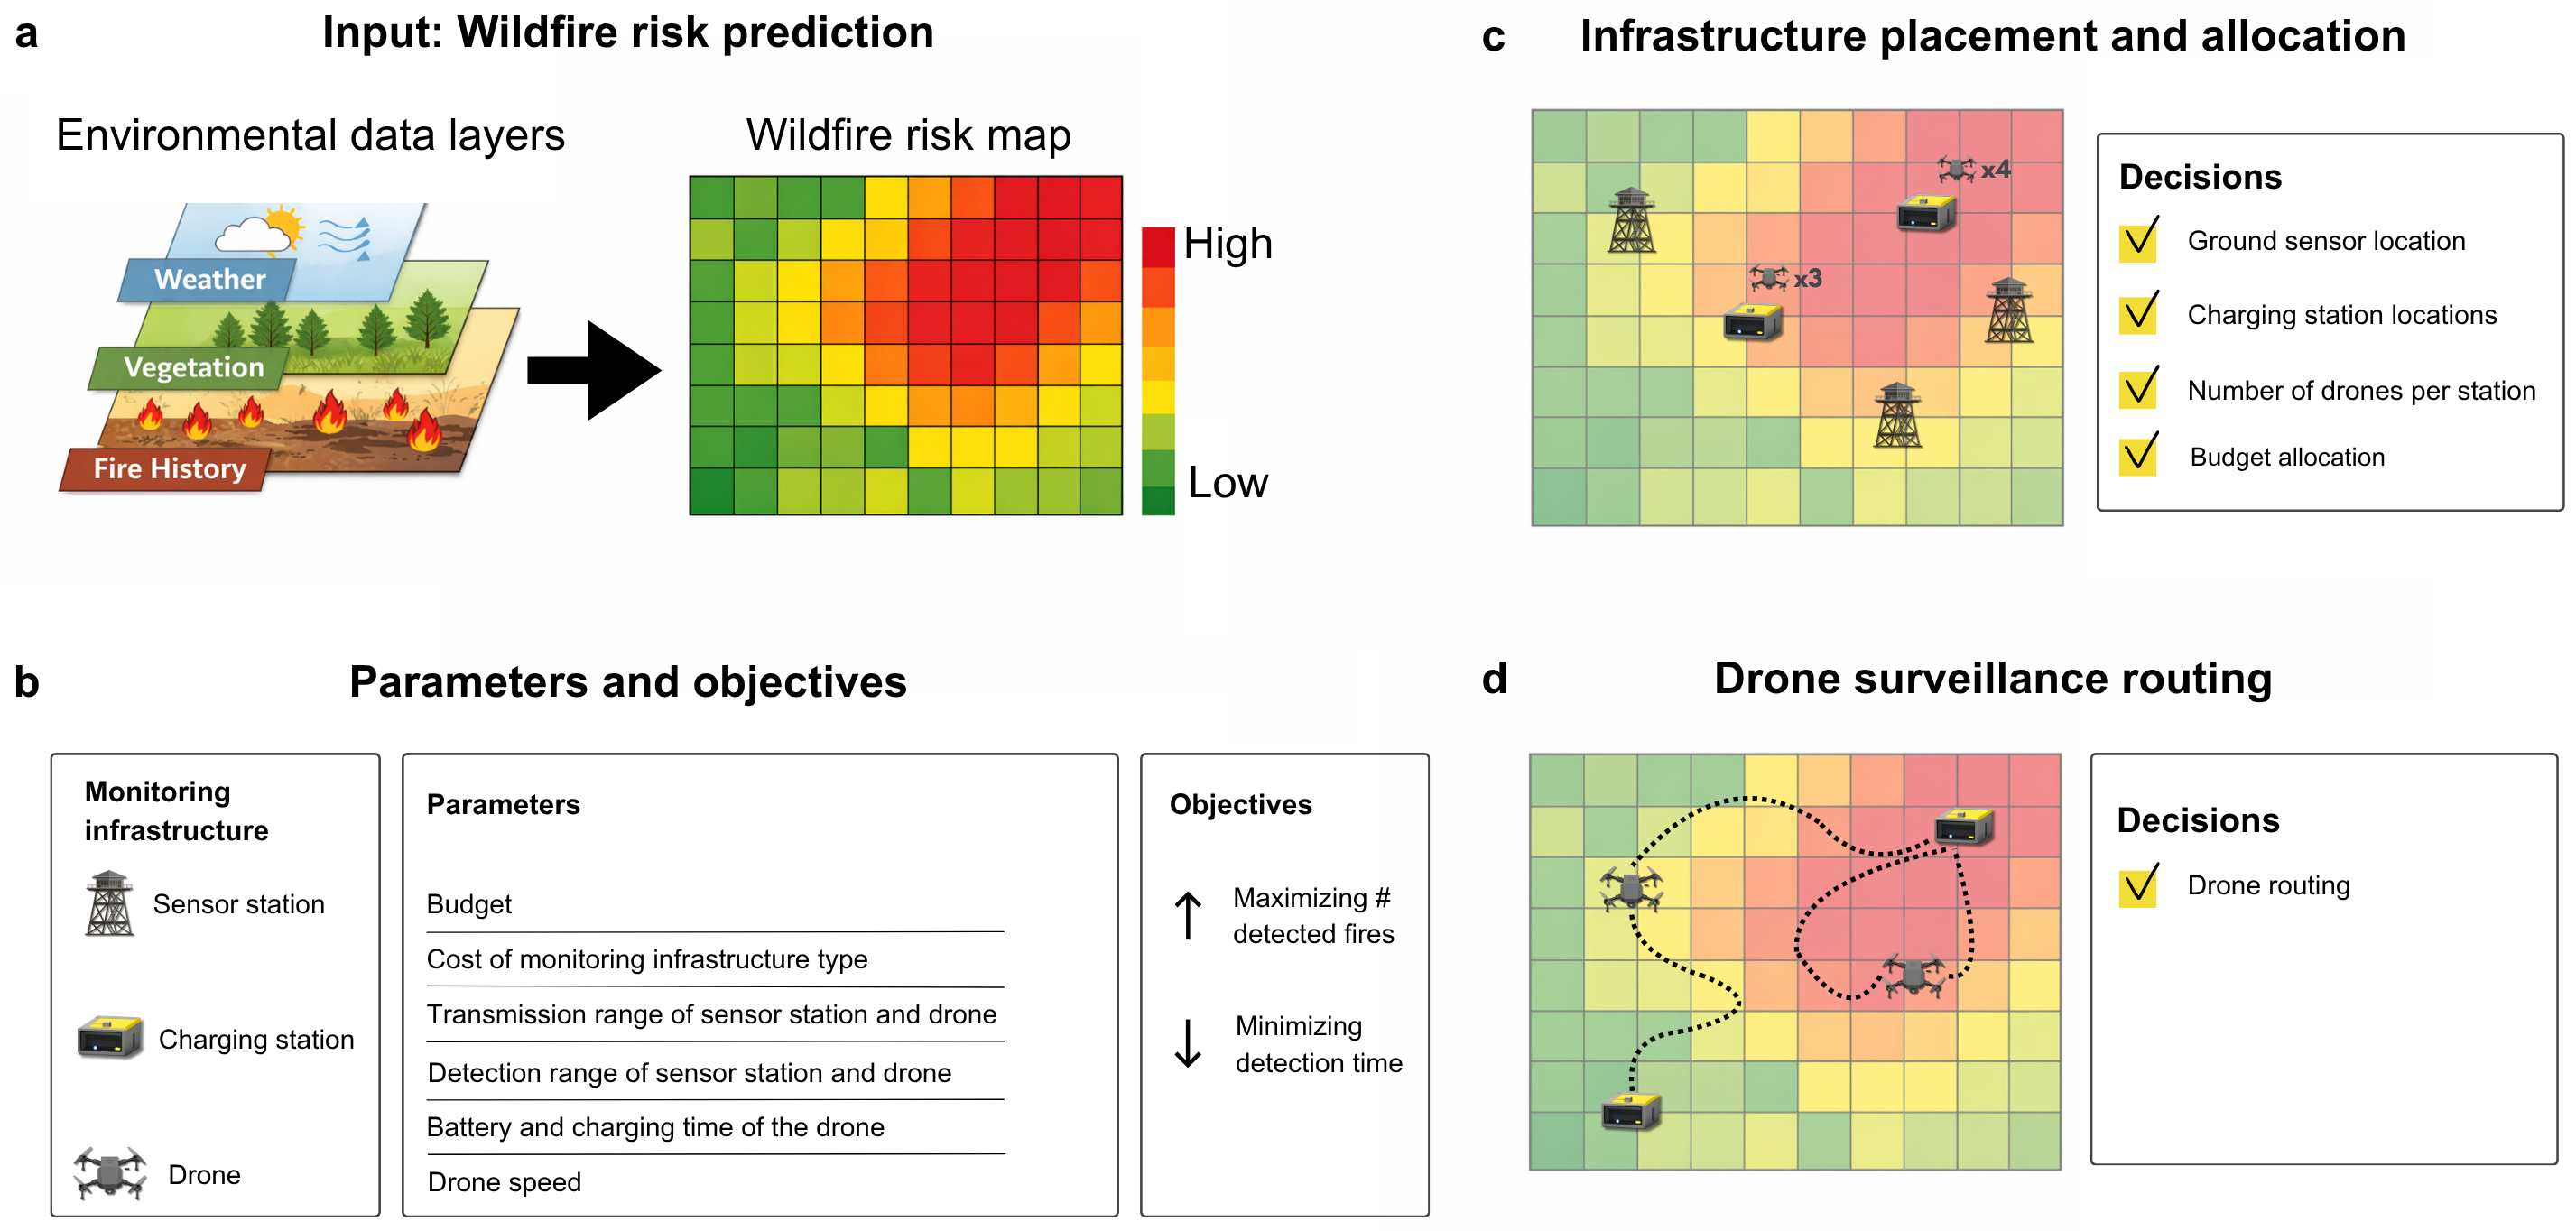
\includegraphics[width=\textwidth,height=0.68\textheight,keepaspectratio]{Figures/High (7).png}
    %     \caption{}
        % \label{fig:framework_a}
    % \end{subfigure}
    % \hfill
    % \begin{subfigure}[t]{0.40\textwidth}
    %     \centering
    %             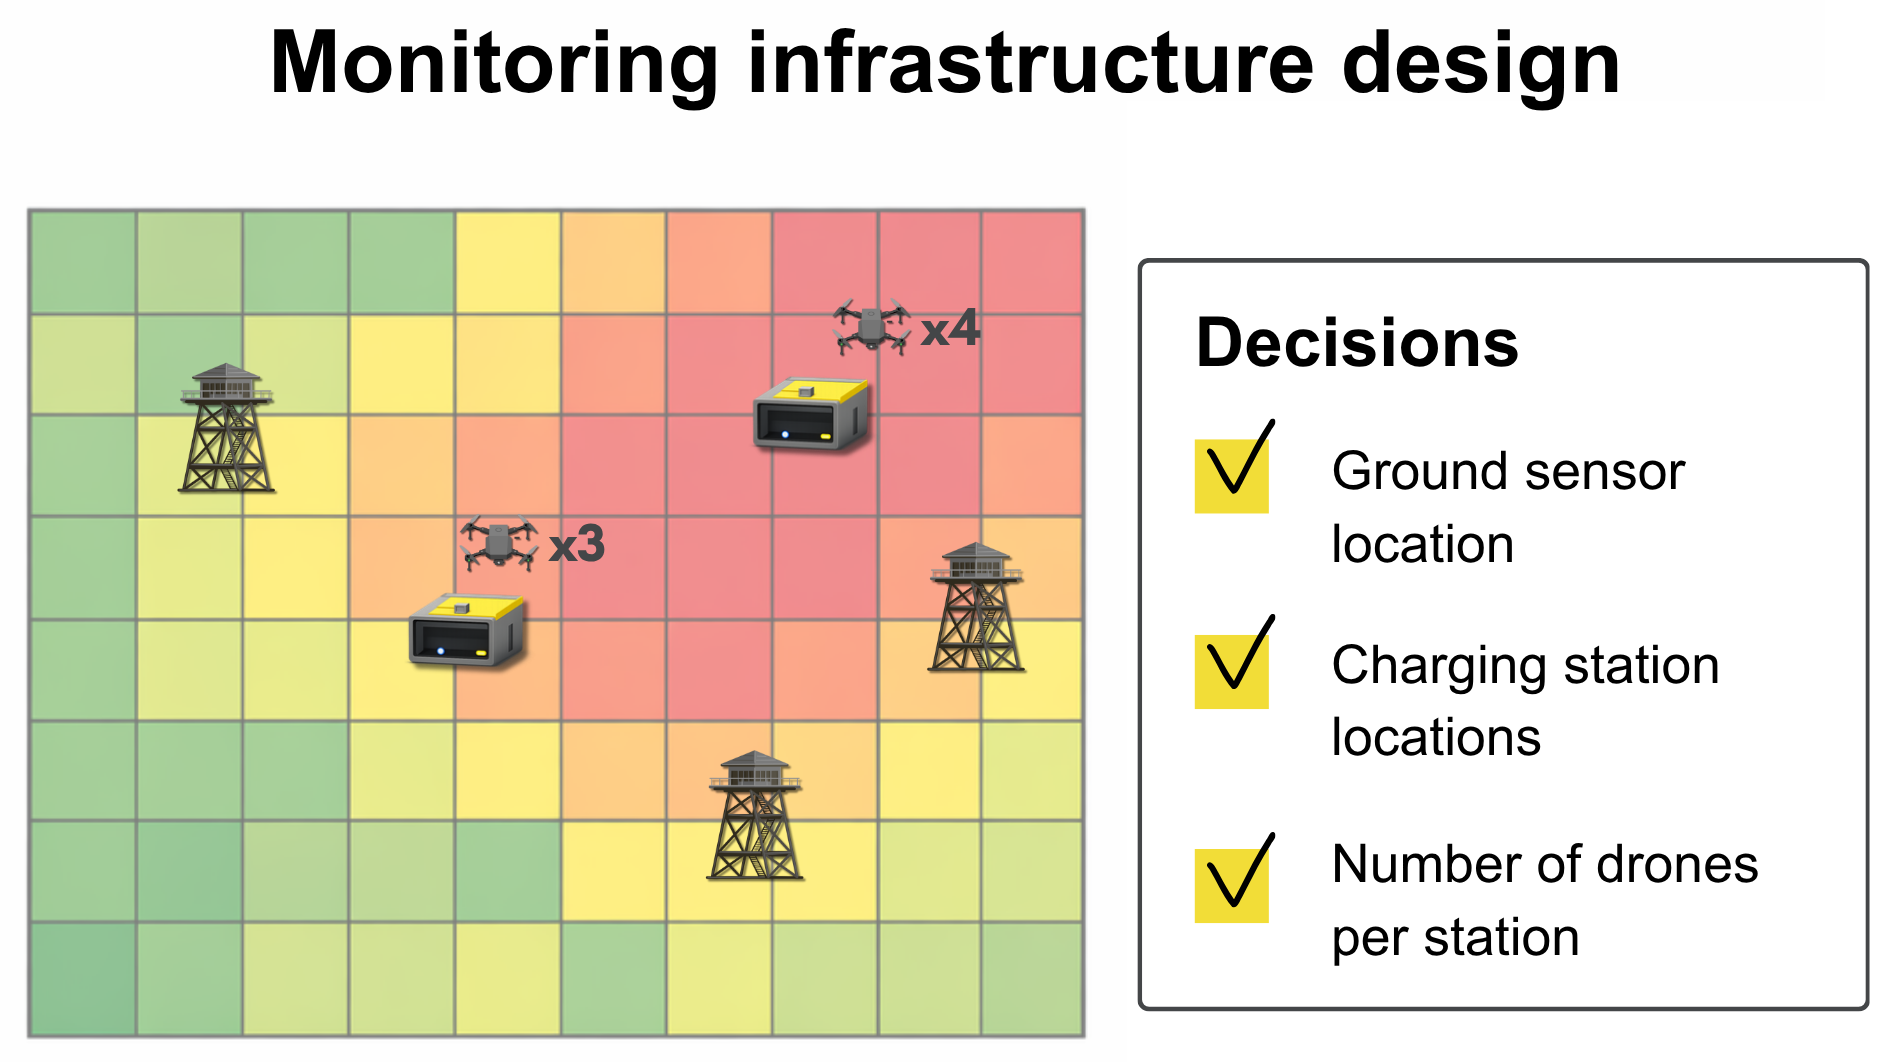
\includegraphics[width=\textwidth]{Figures/High (4).png}
    %     \caption{}
    %     \label{fig:framework_b}
    % \end{subfigure}

    % \vspace{0.5cm}

    % % Second row
    % \begin{subfigure}[t]{0.48\textwidth}
    %     \centering
    %     \includegraphics[width=\textwidth]{Figures/ChatGPT Image Apr 1, 2026, 03_15_24 PM.png}
    %     \caption{}
    %     \label{fig:framework_c}
    % \end{subfigure}
    % % \hfill
    % \begin{subfigure}[t]{0.48\textwidth}
    %     \centering
    %     \includegraphics[width=\textwidth]{Figures/ChatGPT Image Apr 1, 2026, 04_08_38 PM.png}
    %     \caption{}
    %     \label{fig:framework_d}
    % \end{subfigure}
    \caption{\textbf{AI-driven monitoring framework for proactive wildfire detection.} (a) Existing machine-learning models generate spatial wildfire risk maps from environmental data layers, including weather conditions, vegetation characteristics, and historical fire observations. (b) Key operational parameters and optimization objectives define the decision-making framework. (c) Based on the predicted wildfire risk, the monitoring system determines where to deploy sensor  and charging stations, as well as the number of drones allocated to each charging station to form a distributed monitoring network, using budget and infrastructure cost parameters. (d) Drones autonomously patrol the landscape following optimized surveillance routes that account for operational constraints including battery capacity, flight time limits, speed, communication range, and charging requirements.}
    \label{fig:framework}
\end{figure*}

% \blue{The wildfire monitoring framework builds on the computational framework introduced in WFDroneBench, which provides a modular environment for evaluating wildfire monitoring strategies under realistic operational constraints. Here, we extend this methodology to study wildfire detection at statewide scale, focusing on infrastructure design, economic trade-offs, and operational feasibility rather than algorithmic benchmarking.}


The proposed system \blue{builds on the framework introduced in \cite{dronebench2025}} and integrates data-driven wildfire risk prediction, infrastructure design, and autonomous aerial surveillance to enable proactive wildfire detection. \blue{Here, we extend this methodology to study wildfire detection at statewide scale, focusing on infrastructure design, economic trade-offs, and operational feasibility rather than algorithmic benchmarking.}

The framework is built on a spatiotemporal wildfire risk map that captures ignition probabilities across the landscape and is generated using existing machine learning models trained on environmental variables such as vegetation, weather conditions, and historical wildfire observations (Fig. \ref{fig:framework}.a).

The monitoring infrastructure consists of ground sensor stations, charging stations, and drones. Decisions regarding infrastructure placement and drone routing are driven by key operational parameters and optimization objectives, including budget limitations, infrastructure costs, drone battery capacity, charging time, communication and detection ranges, and effective scanning speed, which represents the rate at which drones update grid-level information rather than their raw flight velocity (Fig.~\ref{fig:framework}b). The objective is to minimize wildfire detection time while maximizing the number of fires detected.

 Based on the predicted wildfire risk and the operational parameters, the monitoring infrastructure is optimized by determining the placement of sensor and charging stations, as well as the number of drones assigned to each charging station, forming a distributed monitoring network that prioritizes high-risk regions (Fig.~\ref{fig:framework}c). Given this infrastructure, drones are then routed along optimized surveillance trajectories that balance risk-aware coverage with operational feasibility (Fig.~\ref{fig:framework}d). 
 
 During operation, the risk map is dynamically updated to reflect the mitigating effect of active monitoring, reducing ignition probabilities in regions currently observed by drones or sensors. \blue{Concretely, a surveilled cell's ignition risk is reset to zero and then re-accumulates linearly until the cell is revisited; full details are given in the Methods.} 
% When a wildfire ignition occurs, detections are triggered through aerial or ground-based observations, marking the point at which emergency response actions can be initiated (Fig.~1d). \\
\captionsetup[subfigure]{
    labelformat=simple,
    labelsep=space,
    font=bf,
    skip=1pt
}
\renewcommand\thesubfigure{\textbf{\alph{subfigure}}}

% \subsection*{California dataset}
To evaluate the proposed framework, we construct a case study based on the state of California. California is used as a representative case study due to the availability of extensive historical wildfire records and environmental datasets; however, the proposed framework is general and can be deployed in other geographic regions, including those with more limited data availability. 

% \subsection*{Near-complete early wildfire detection is achievable in minutes within current budget levels}
\blue{\subsection*{Near-complete wildfire detection in minutes}}
\noindent With a \$100 million budget, our optimized drone monitoring network detects 97.3\% (95\% CI: 96.7--97.8\%) of California wildfires across 2021--2024, with 74\% of detections occurring within the first hour of ignition ($\Delta t = 0$) and all but one detected fire identified within four hours (Fig.~\ref{fig:frontier}, Table~\ref{tab:detection}). This budget is well below California's current expenditure on wildfire resource management and fire prevention, estimated at \$440 million for 2024--25~\cite{next10_rebuilding_resilient_2021}, and represents a fraction of the economic losses caused by a single major fire event. These results indicate that near-complete, rapid wildfire detection across California is technically feasible and financially within reach under realistic operational assumptions.

The detection frontier quantifies how this capability scales with investment (Fig.~\ref{fig:frontier}). At \$20 million, the network covers only a concentrated band of Northern and Central California and detects 30.9\% of benchmark fires. At \$50 million, detection rises to 60.0\%, and at \$75 million to 91.2\%. The curve steepens sharply through this range, then flattens above approximately \$100 million, where the network spans the majority of the state's burnable landscape and additional spending yields diminishing returns. This nonlinearity reflects the underlying spatial coverage dynamic illustrated in Fig.~\ref{fig:placement}. At \$20 million, 69\% of all 3{,}693 historical California ignitions across 2021--2024 fall outside the network's reach entirely (out of sensor coverage and unreachable by drones); by \$100 million, that fraction drops to 3\%, with 3{,}596 of 3{,}693 historical fires discoverable. Empirically, once a fire falls within drone range, detection is nearly guaranteed: detection rates among reachable fires consistently exceed 95\% for the best-performing strategy across all budget levels (Table~\ref{tab:detection}). At the \$500 million budget, where every historical ignition is discoverable, the single fire left undetected by the team-orienteering strategy is an artifact of an inconsistency between datasets: the USFS record places this ignition on a lake, a location our risk map assigns an ignition probability of 0 and therefore never visits. This anecdotal misalignment on open water accounts for the sole missed fire at full coverage.

\begin{figure*}[!t]
    \centering
        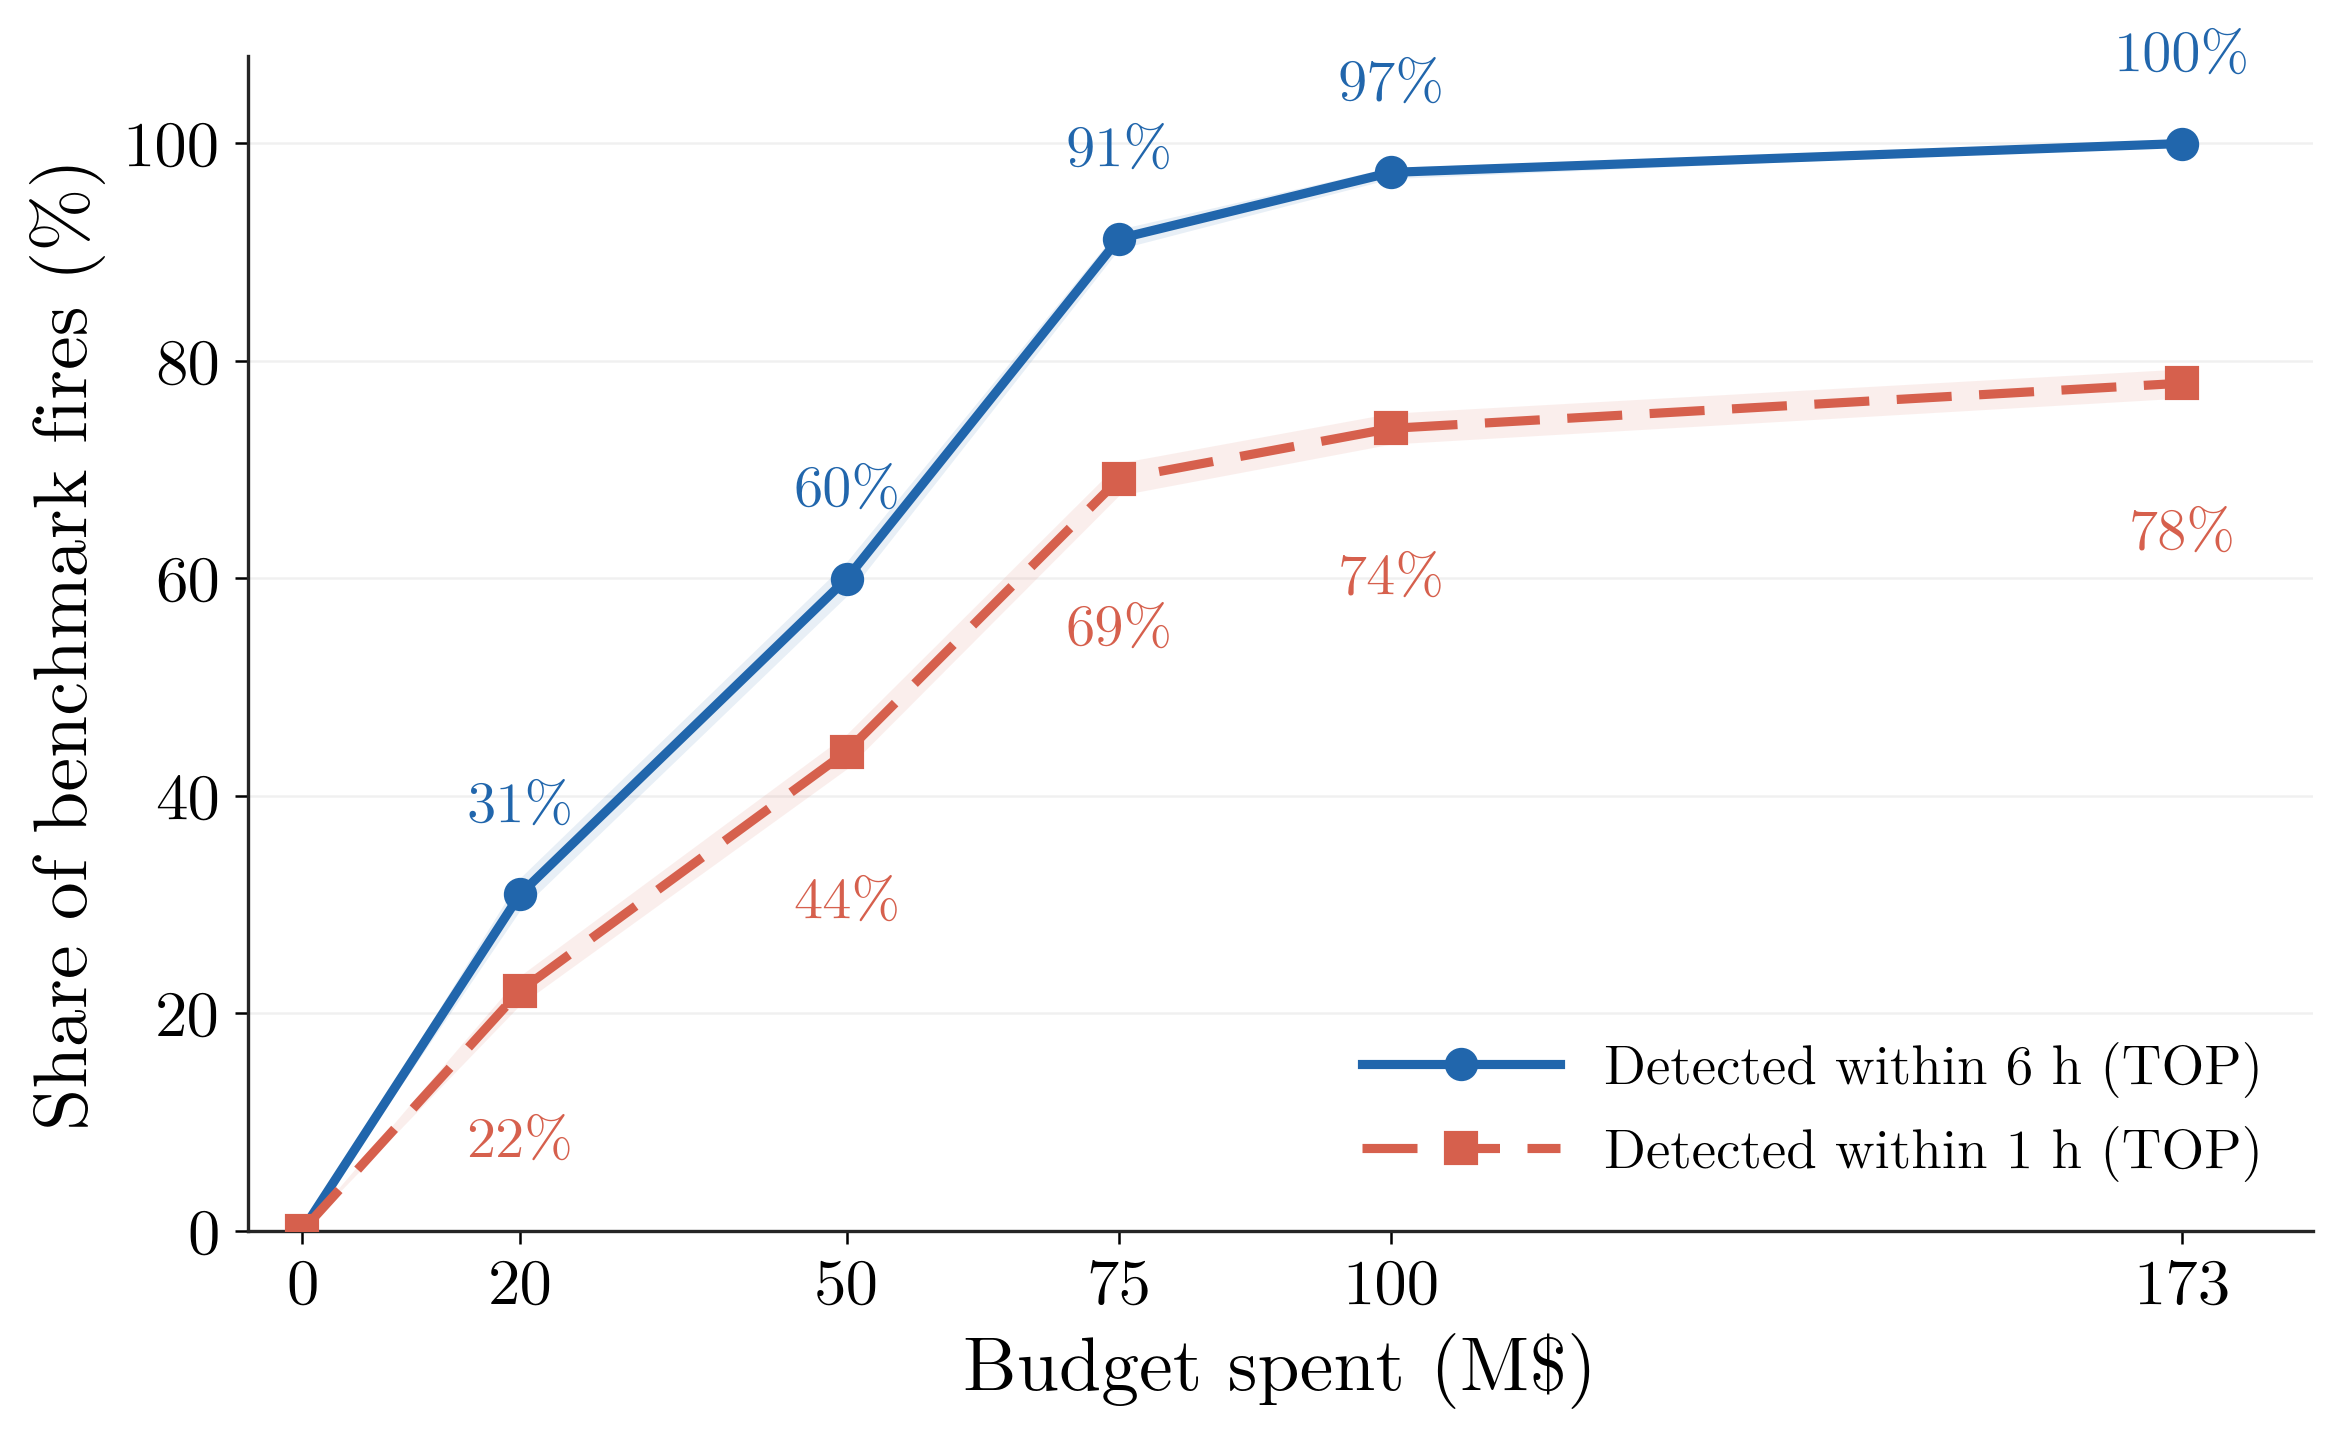
\includegraphics[width=\linewidth,height=0.62\textheight,keepaspectratio]{Figures/frontier.png}
        \caption{\textbf{Detection rate and speed as a function of monitoring investment.} Percentage of California wildfire ignitions across 2021--2024 ($n = 3{,}693$ fires, pooled) detected within six hours of ignition (blue) and within the first hour ($\Delta t = 0$, orange) for the team orienteering (TOP) routing strategy, as a function of realized hardware spend. Detection rates are computed over the full pooled fire population across all four years rather than by averaging per-year rates. Five budget levels are shown: \$20M, \$50M, \$75M, \$100M, and \$500M. Shaded bands are 95\% Wilson confidence intervals. Budget cap for each spend level is shown in parentheses on the x-axis.}
        % Detection rates for the other two routing strategies are reported in Table~\ref{tab:detection}; corresponding infrastructure layouts are shown in Fig.~\ref{fig:placement}.
        \label{fig:frontier}
\end{figure*}

% Table 1 — Detection rates across strategies and budgets (2021–2024, pooled over all fires)
% Generated by paper/Nature_Wildfires/scripts/build_table1_detection.py
% Pooled per-fire across years (75M: 20260522_170454; 500M eps1 + T20 ground-sensor opt-cell fix: 20260523_212551_sensorfix; others: 20260520_062339)
% Confidence intervals: 95% Wilson score interval on the pooled fire population
\begin{table}[!t]
\caption{Detection performance across routing strategies and deployment budgets,
  pooled over California wildfire years 2021\textendash2024 (\(n = 3,692\textendash3,693\) fires per cell).
  Rates are computed over the full pooled fire population, not by averaging per-year rates.
  \emph{Det.\ rate}: overall detection rate with 95\% Wilson score interval.
  \emph{Within 1\,h}: share of all fires detected in the first simulation step (\(\Delta t = 0\)).
  \emph{Mean $\Delta t$}: mean detection delay (hours) over detected fires only.}
\label{tab:detection}
\begin{tabular}{@{}llrrrr@{}}
\toprule
Budget & Strategy & Det.\ rate (\%) & Within 1\,h (\%) & Mean $\Delta t$ (h) & $n$ fires \\
\midrule
\$20M & TOPGrowing     & 30.9 [29.5, 32.4] & 22.1 & 0.33 & 3693 \\
 & MaxCov         & 29.5 [28.1, 31.0] & 17.2 & 0.51 & 3693 \\
 & LinearMinTime  & 25.9 [24.5, 27.3] & 18.4 & 0.52 & 3693 \\
\addlinespace
\$50M & TOPGrowing     & 60.0 [58.4, 61.5] & 44.1 & 0.29 & 3693 \\
 & MaxCov         & 57.0 [55.4, 58.6] & 32.7 & 0.56 & 3693 \\
 & LinearMinTime  & 46.1 [44.5, 47.8] & 33.0 & 0.52 & 3693 \\
\addlinespace
\$75M & TOPGrowing     & 91.2 [90.3, 92.1] & 69.1 & 0.27 & 3692 \\
 & MaxCov         & 87.1 [86.0, 88.1] & 51.1 & 0.52 & 3693 \\
 & LinearMinTime  & 79.9 [78.6, 81.2] & 56.9 & 0.52 & 3693 \\
\addlinespace
\$100M & TOPGrowing     & 97.3 [96.7, 97.8] & 73.8 & 0.27 & 3692 \\
 & MaxCov         & 92.7 [91.8, 93.5] & 53.9 & 0.52 & 3693 \\
 & LinearMinTime  & 84.5 [83.3, 85.6] & 61.8 & 0.46 & 3693 \\
\addlinespace
\$500M & TOPGrowing     & 100.0 [99.8, 100.0] & 77.9 & 0.24 & 3693 \\
 & MaxCov         & 96.6 [96.0, 97.1] & 60.2 & 0.46 & 3693 \\
 & LinearMinTime  & 84.3 [83.1, 85.4] & 64.9 & 0.41 & 3693 \\
\bottomrule
\end{tabular}
\end{table}


% Two-column figure*: if only [!t] is used while the top area is saturated, or if the float
% is taller than a float page, LaTeX may defer it to the end. dblfloatfix (preamble) plus [!tb]
% and slightly smaller panels help Fig.~\ref{fig:placement} stay near the narrative.
\begin{figure*}[!tb]
    \centering \includegraphics[width=\textwidth,height=0.66\textheight,keepaspectratio]{Figures/placement_composite.png}
    \caption{\textbf{Optimized deployment of monitoring infrastructure and fire discoverability across budget scenarios in California.} Fires are labeled as discoverable if the drones can reach them given their battery starting from any charging station. Discoverability is computed over all 3{,}693 historical California ignitions across 2021--2024. At \$20~million, 40~stations and 280~drones are deployed, concentrated in Northern and Central California; 31\% of historical fires are discoverable. At \$50~million, 100~stations and 700~drones expand coverage to 60\% of benchmark fires. At \$100~million, 200~stations and 1{,}400~drones span the majority of the state's burnable landscape; 97\% of historical fires are discoverable. At \$500~million budget 339~charging stations, 31~ground sensors, and 2{,}373~drones are deployed at a realized hardware cost of \$172.6~million; all historical ignitions are discoverable.}
    \label{fig:placement}
\end{figure*}

% \subsection*{Ground sensors are economically dominated by drone-based monitoring}
\blue{\subsection*{Drones dominate ground sensors economically}}
\noindent Across all budget levels below \$500 million, the placement optimizer allocates zero ground sensors, devoting the entire infrastructure budget to charging stations and drones. Under the cost parameters of our experiments (Table~\ref{tab:benchmark_params}), a single charging station equipped with seven drones costs \$0.50 million and can scan approximately 1{,}225~km$^2$ within one battery cycle, roughly ten times cheaper per unit area than an equivalent ground sensor deployment. Ground sensors only appear at the \$500 million cap, and only to close the small residual gaps that remain at the periphery of the drone network once full-state coverage is otherwise achieved (Fig.~\ref{fig:placement}, panel~\textbf{d}).

This finding is sensitive to cost assumptions: a substantial reduction in ground sensor costs, or an increase in drone operating expenses, would shift the optimal balance toward more sensor-heavy deployments. Under current technology costs \blue{(more details in Methods)}, however, drones economically dominate static sensors for landscape-scale wildfire monitoring.

\paragraph{Cost sensitivity.}
We varied only the unit cost assumed for a ground sensor installation, holding charging-station and drone costs at the values in Table~\ref{tab:benchmark_params} and re-solving the same placement optimization model as in our previous experiments. At total budgets of \$20 million and \$50 million we observe three qualitative regimes in the optimal infrastructure mix as the ground-sensor unit cost varies (Fig.~\ref{fig:breakeven_costsensitivity}). When static sensors are very inexpensive, the budget is devoted almost entirely to dense ground coverage and no charging stations are deployed. At intermediate unit costs, ground sensors, charging stations, and drones coexist: aerial infrastructure extends reachable surveillance while static units remain where they are still comparatively cost-effective. When static units become sufficiently expensive, the optimal portfolio uses only charging stations and drones. The price interval over which mixed deployments arise is narrow at \$20 million (illustrated between approximately \$10{,}000 and \$12{,}000 per ground sensor in our scan) but substantially wider at \$50 million, where mixed portfolios persist from roughly \$11{,}000 to about \$22{,}000 per sensor. Our benchmark parameterization of \$100{,}000 per ground sensor (Table~\ref{tab:benchmark_params}) lies far above this coexistence band, which is consistent with the drone-heavy infrastructure choices reported above.

\begin{figure*}[!tb]
    \centering
    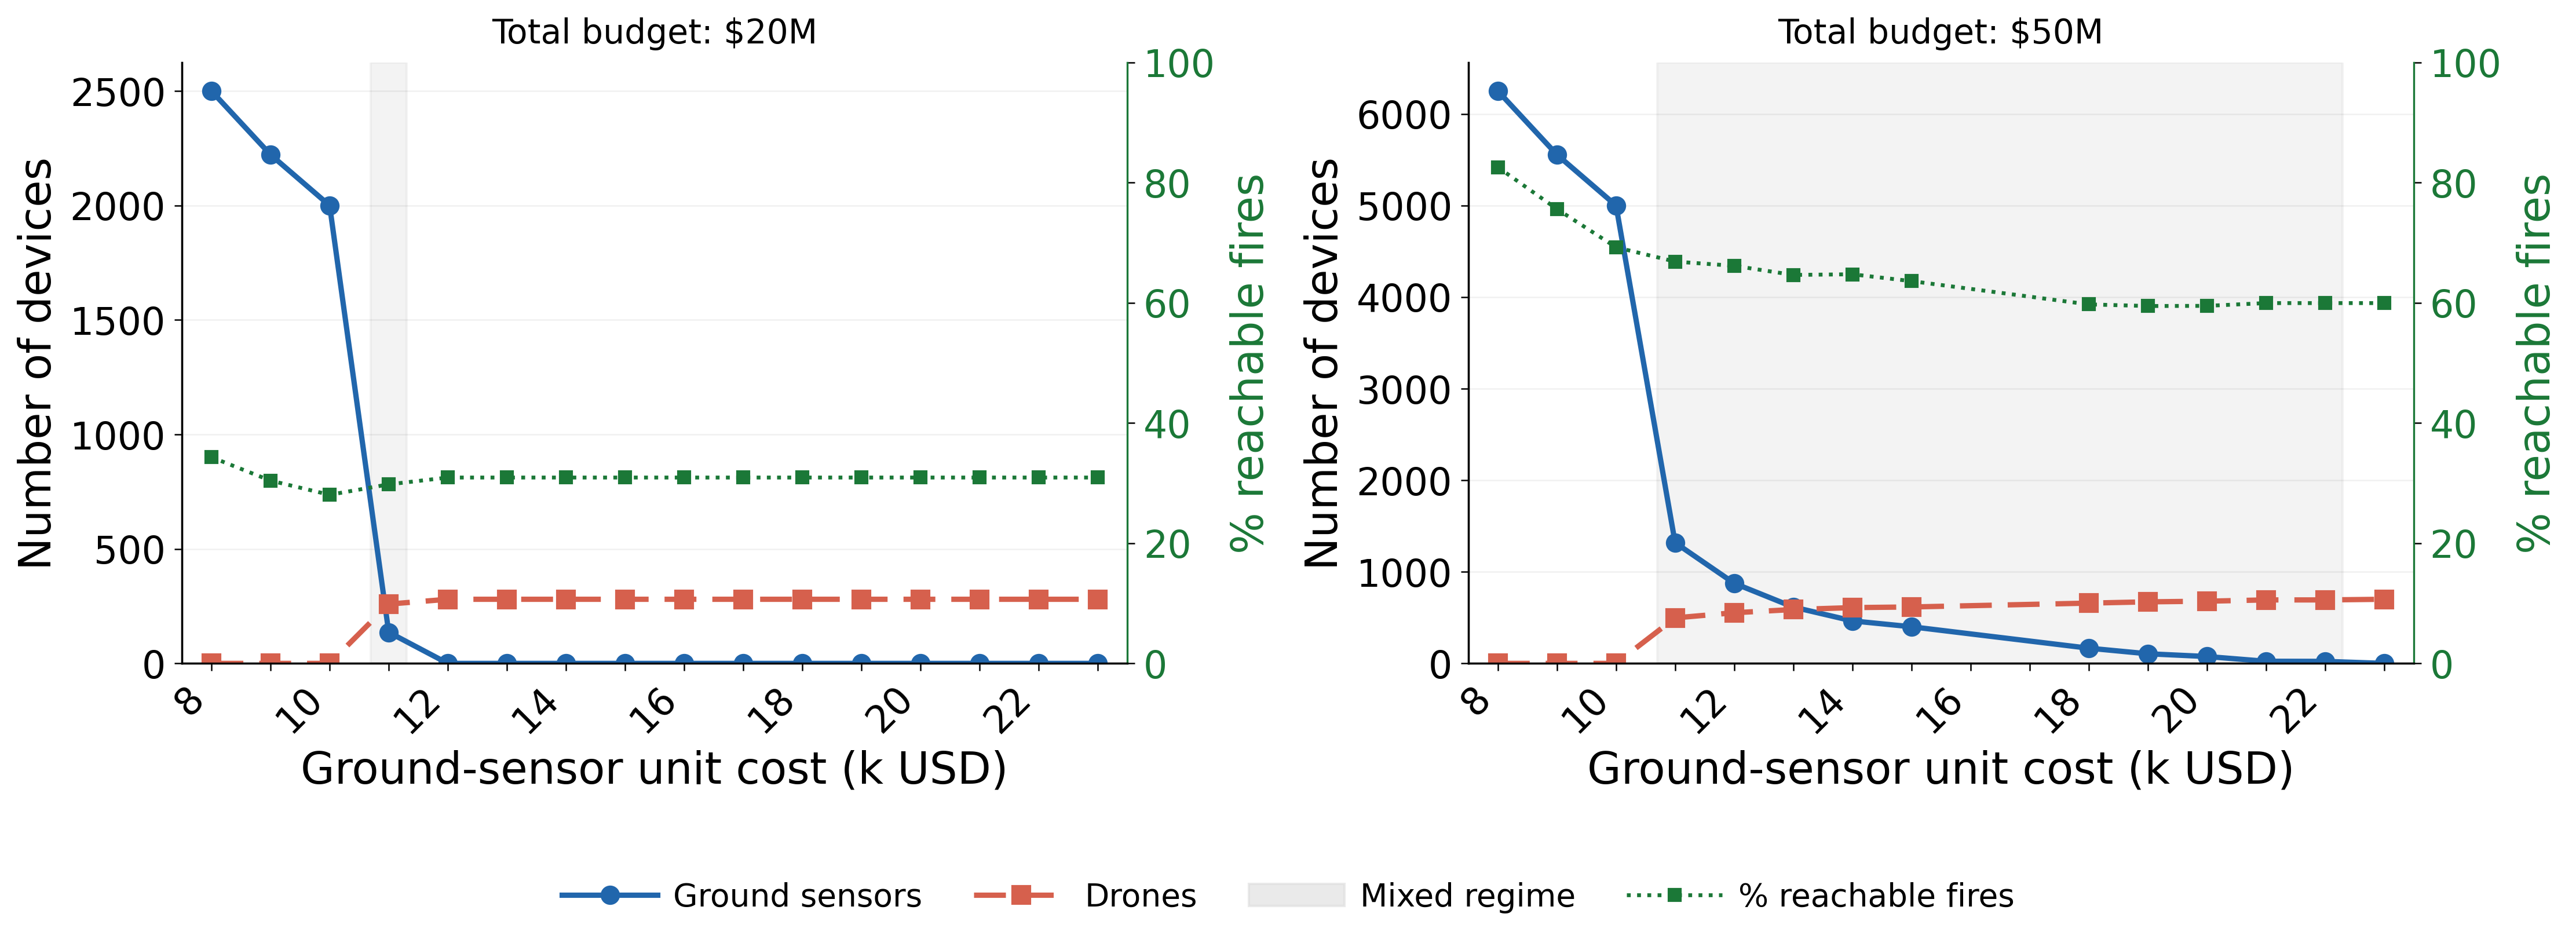
\includegraphics[width=\linewidth,height=0.60\textheight,keepaspectratio]{Figures/breakeven_costsensitivity_lines.png}
    \caption{\textbf{Cost sensitivity of the optimal infrastructure mix to ground-sensor unit cost.} Optimal device counts as the assumed ground-sensor unit cost is varied, at total budgets of \$20~million (left) and \$50~million (right), with charging-station and drone unit costs held fixed at Table~\ref{tab:benchmark_params}. \textbf{Left axis:} number of ground sensors (blue, solid) and drones (orange, dashed) in the optimal placement. \textbf{Right axis} (green, dotted): share of California wildfire ignitions across 2021--2024 reachable by the resulting network ($n = 3{,}693$ fires). The shaded band marks the \emph{mixed regime}, where ground sensors, charging stations, and drones coexist in the optimum: it is narrow at \$20~million (around USD~11k per sensor, switching to a drones-only portfolio by USD~12k) and substantially wider at \$50~million (roughly USD~11k--22k, drones-only from USD~23k).}
    \label{fig:breakeven_costsensitivity}
\end{figure*}


% \subsection*{Routing strategy affects detection speed more than detection rate}
\blue{\subsection*{Routing strategy primarily affects detection speed}}
We evaluate three drone routing strategies: team orienteering (TOP), which maximizes the number of distinct high-risk locations visited per battery cycle; maximum coverage (MaxCov), which prioritizes surveillance of high-risk areas; and detection-time minimization (LinearMinTime), which concentrates patrols on the highest-risk cells to reduce detection delay \blue{(details in Methods)}. Across all budget levels, TOP achieves the highest overall detection rates, with the difference most pronounced at intermediate budgets. At \$100 million, TOP detects 97.3\% of benchmark fires versus 92.7\% for MaxCov and 84.5\% for LinearMinTime (Table~\ref{tab:detection}).

The key structural finding is that routing strategy governs detection speed, while placement governs detection rate. Among fires within drone reach, detection is nearly guaranteed by any strategy; what varies is how quickly the fire is found. \blue{From Table \ref{tab:detection} we observe that,} at \$100 million, 74\% of fires detected by TOP are identified within the first hour ($\Delta t = 0$), compared with 54\% for MaxCov (Mann-Whitney $U$ test on $\Delta t$ values among jointly detected fires, $p < 0.001$). LinearMinTime, despite being explicitly designed to minimize detection delay, detects fewer fires overall because its patrol concentration leaves peripheral locations undervisited. Placement is therefore the binding constraint: extending the network's geographic footprint matters more than how drones are routed within it.

% \subsection*{The optimized drone network substantially outperforms the ALERTCalifornia camera baseline}
\blue{\subsection*{Optimized drones exceed an idealized incumbent ALERTCalifornia system}}

\noindent California's ALERTCalifornia program operates a statewide network of 699 unique fixed near-infrared camera sites on elevated terrain~\cite{alertcalifornia2026}. We estimate the total public investment in the ALERTCalifornia program at US\$50--100~million\footnote{A documented 2024--25 state appropriation of \$10.4M~\cite{california_ab108_2024,
govtech_insider_calfire_ucsd_2024} represents a single fiscal year; total
cumulative investment is substantially larger given multi-year CAL~FIRE
contributions, NSF funding of the HPWREN predecessor network since
2001~\cite{alertcalifornia_history}, and private sponsorship from PG\&E and
Digital Path~\cite{alertcalifornia_time2023}. Extrapolating \$5--10M\,yr$^{-1}$
in operating costs over a $\sim$10-year expansion period and \$10--20M in
capital expenditure for 1,200+ camera installations at \$8,000--15,000 per unit
(authors' estimate) yields the \$50--100M order-of-magnitude range. No
consolidated budget figure has been published by the
program~\cite{alertcalifornia2026}.}
We use this network as a static-sensor baseline, evaluated against the same California ignition records used throughout (2021--2024; per-year $n$ in Table~\ref{tab:alertcalifornia}). A fire is counted as detected if its ignition cell centre lies within a Euclidean radius $r$ of at least one camera site. We emphasize that this is a deliberately \emph{optimistic} model of camera performance: it assigns probability-one detection to any ignition within radius, ignoring line-of-sight occlusion by terrain, atmospheric attenuation, and the program's confirmation/ML-alerting layer. It therefore yields an \emph{upper bound} on what the fixed-camera geometry can achieve, and any comparison in which the drone network exceeds it is correspondingly conservative. Optical cameras mounted at fixed elevations have effective detection ranges that depend on terrain, atmospheric conditions, and fire characteristics; ALERTCalifornia reports a sight range of $60$ miles on a clear day, but this does not correspond to a probability of detection of 1 for any fire within this radius. Their online coverage visualization tool displays a radius on $20$ miles. For our baseline experiments, we therefore simulate detection rates across a range of assumed radii from $5$ to $50$ km and report the results in Table~\ref{tab:alertcalifornia}. Fig.~\ref{fig:alertcalifornia} maps camera coverage at $r = 10$~km and $r = 32$~km ($\sim20$ miles).

\begin{table}[!t]
\caption{\textbf{ALERTCalifornia camera-network detection per year.} For each detection radius and year, we report the share of California wildfire ignitions whose location falls within the radius of at least one camera (an upper bound on detection, since within-radius detection is assumed certain), with 95\% Wilson confidence intervals. Computed on the full California fire datasets (one column per year; 2024 is fully out-of-sample).}
\label{tab:alertcalifornia}
{\small
\begin{tabular}{@{}lcccc@{}}
\toprule
\textbf{Radius} & \textbf{2021} (n=981) & \textbf{2022} (n=903) & \textbf{2023} (n=992) & \textbf{2024} (n=817) \\
\midrule
5\,km & 19.6\% [17.2, 22.2] & 20.3\% [17.8, 23.0] & 19.2\% [16.8, 21.7] & 18.5\% [16.0, 21.3] \\
10\,km & 45.3\% [42.2, 48.4] & 52.4\% [49.1, 55.6] & 45.4\% [42.3, 48.5] & 49.8\% [46.4, 53.2] \\
20\,km & 78.8\% [76.1, 81.2] & 83.8\% [81.3, 86.1] & 75.9\% [73.1, 78.5] & 83.5\% [80.8, 85.9] \\
32\,km & 90.7\% [88.7, 92.4] & 95.1\% [93.5, 96.4] & 91.7\% [89.9, 93.3] & 92.8\% [90.8, 94.4] \\
50\,km & 100\% [99.6, 100] & 100\% [99.6, 100] & 100\% [99.6, 100] & 100\% [99.5, 100] \\
\bottomrule
\end{tabular}
}
\end{table}


% Results paragraph on ALERTCalifornia leakage:
\paragraph{Out-of-sample evaluation and ALERTCalifornia leakage.}
The ALERTCalifornia camera network has been deployed and progressively expanded
between 2017 and 2024, with camera siting partially informed by historical
ignition records that include fires from 2021--2023~\cite{alertcalifornia_history,alertcalifornia2026}.
This means that the 2021--2023 columns of Table~\ref{tab:alertcalifornia} probe
the network \emph{partly in-sample} from a siting-decision standpoint. The 2024
column provides the cleanest out-of-sample evaluation, given that the 2024
ignition data were not available when most camera placement decisions were made,
and we therefore use the 2024 dataset for Figure~\ref{fig:alertcalifornia}.

% Same float placement as Fig.~\ref{fig:placement}: [!tb] + slightly reduced height (dblfloatfix in preamble).

% Same float placement as Fig.~\ref{fig:placement}: [!tb] + slightly reduced height (dblfloatfix in preamble).
\begin{figure*}[!t]
    \centering
    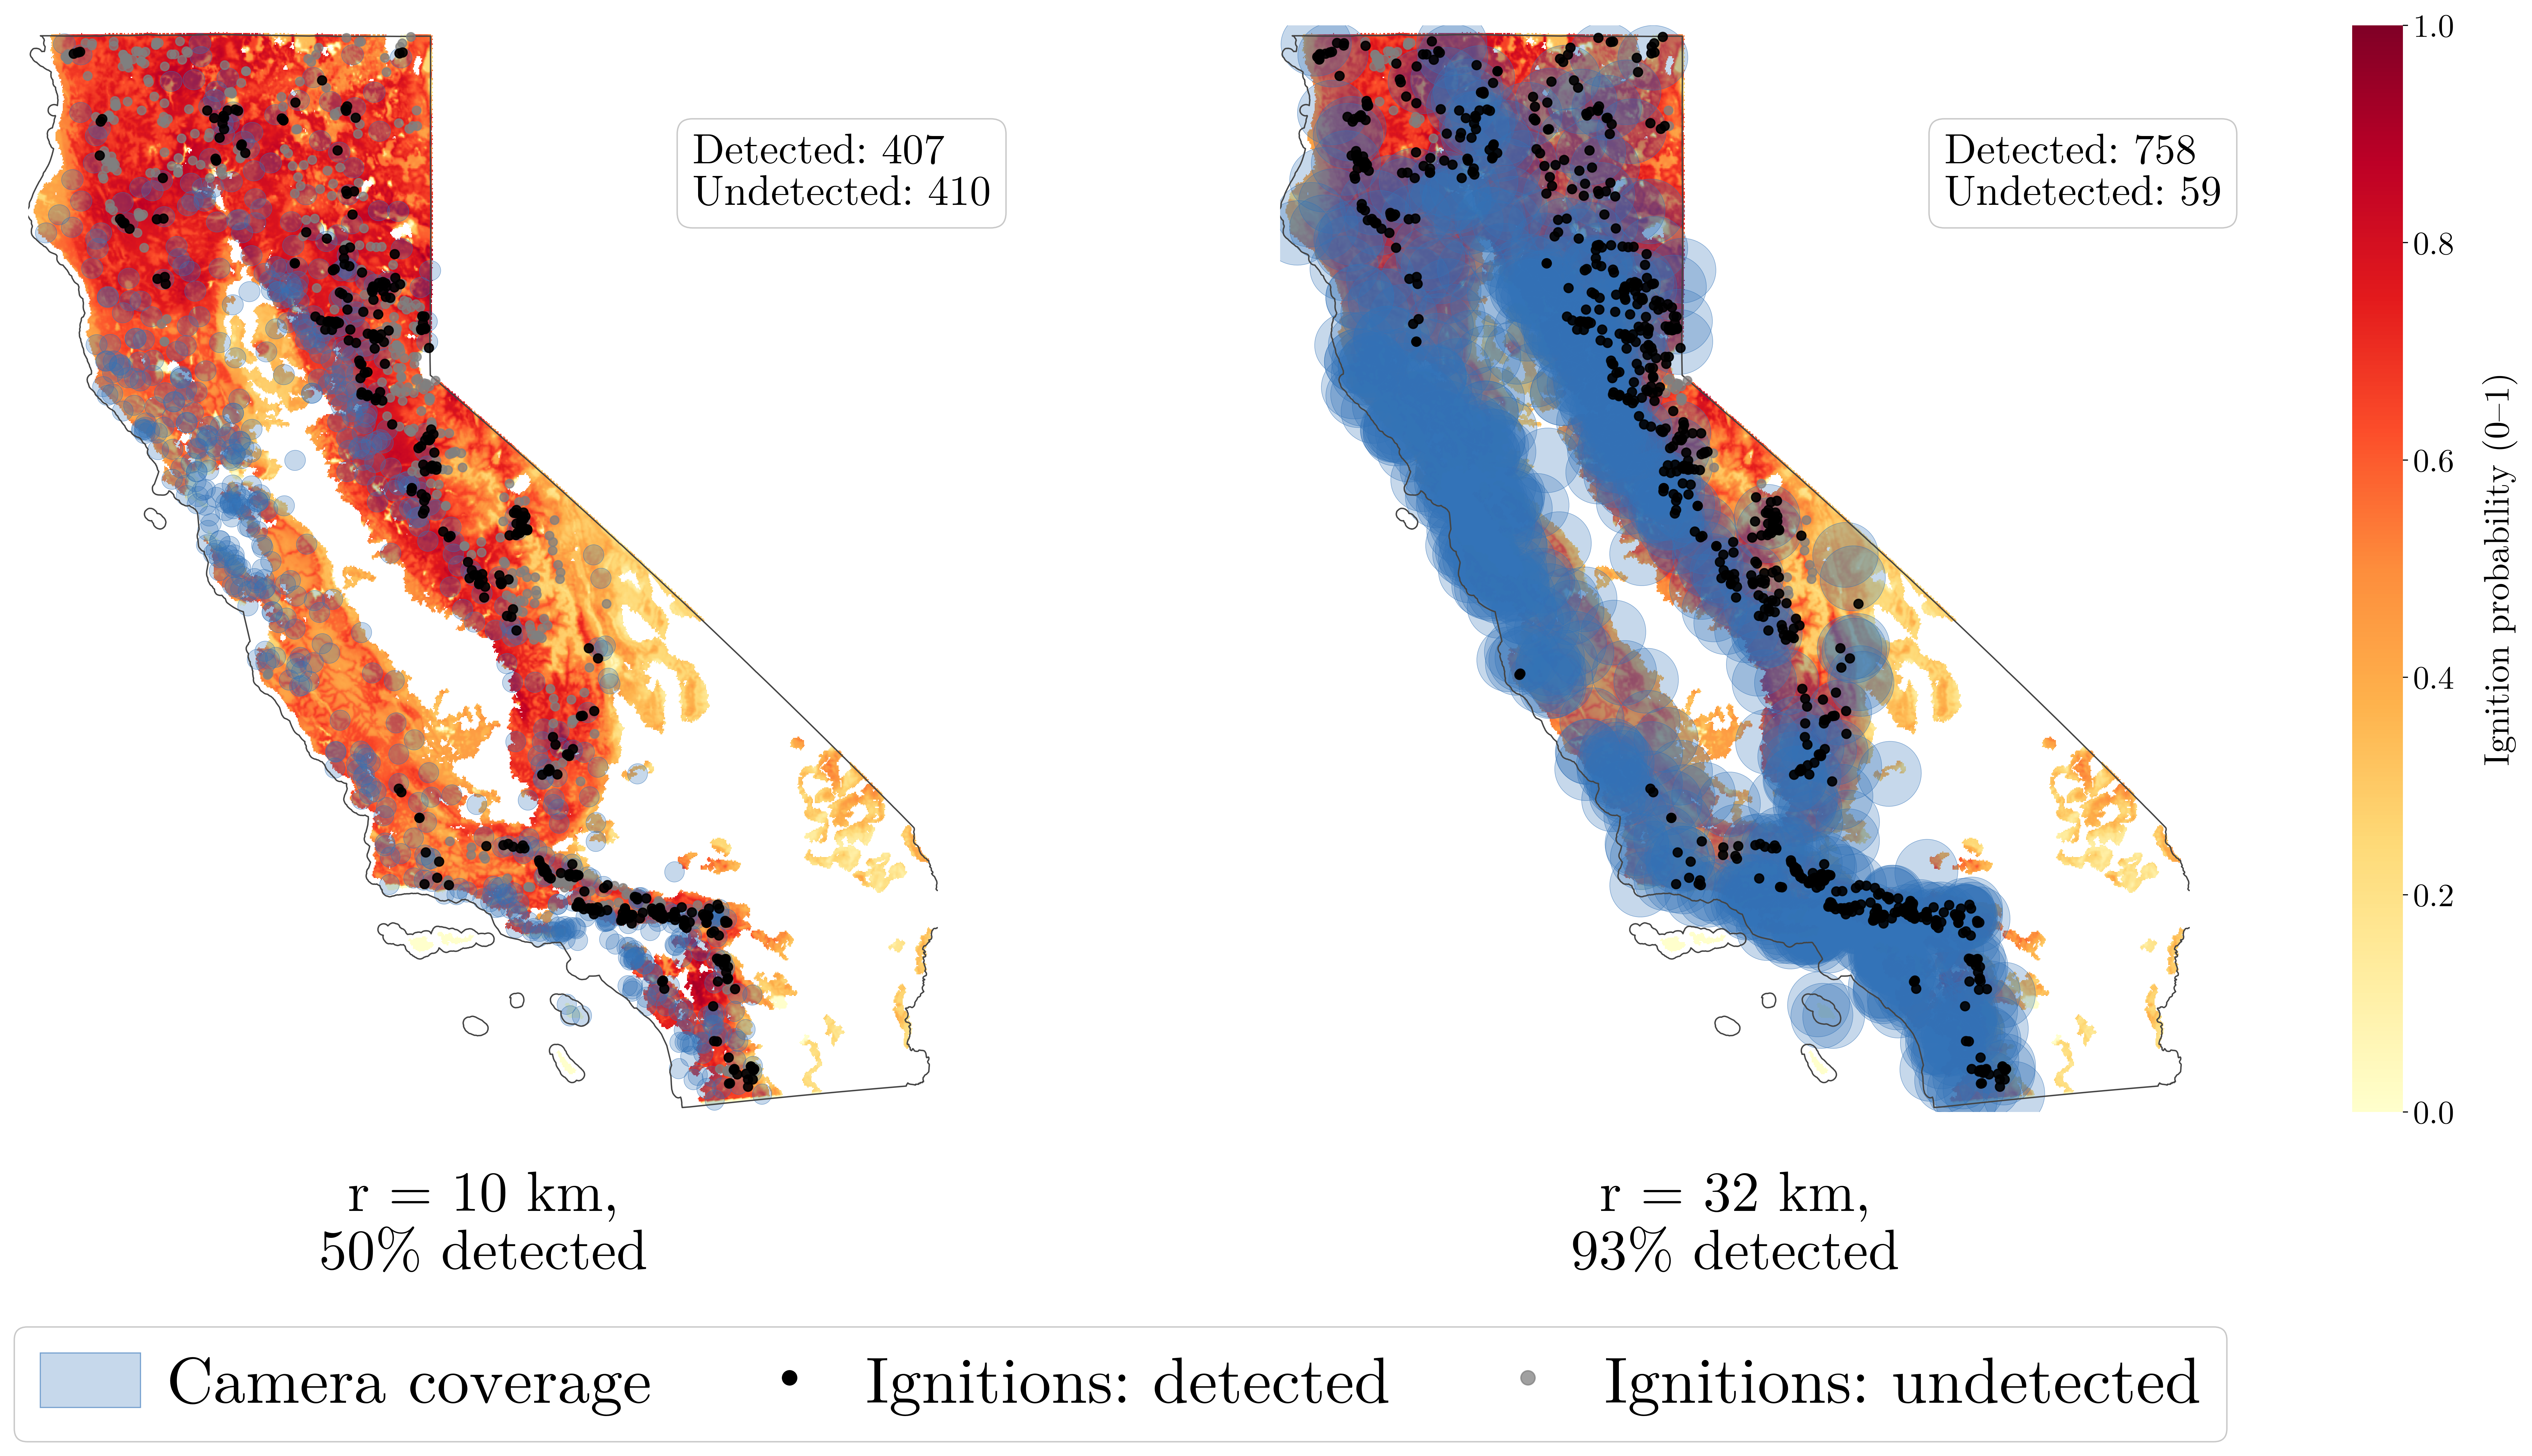
\includegraphics[width=\textwidth,height=0.62\textheight,keepaspectratio]{Figures/alertcalifornia_coverage_composite.png}
    \caption{\textbf{ALERTCalifornia camera coverage of California 2024 wildfire ignitions ($n = 817$).}
Blue regions indicate the assumed camera detection range around each ALERTCalifornia site at 10~km and 32~km radii. Black dots denote detected ignitions and gray dots denote undetected ignitions. The 2024 dataset provides the cleanest out-of-sample evaluation, as these fires postdate the camera siting decisions.}
    \label{fig:alertcalifornia}
\end{figure*}

On the fully out-of-sample 2024 ignitions ($n = 817$), the geometric camera model detects 49.8\% of fires at a 10~km radius and 92.8\% even at the optimistic 32~km sector range (Table~\ref{tab:alertcalifornia}). Because this model already credits the cameras with perfect within-radius detection, these figures are upper bounds. On the same 2024 fires, the optimized drone network at \$100~million detects 97.2\% (95\% CI: 95.8--98.1\%), exceeding even the most generous camera-coverage geometry. 

%\caption{\textbf{ALERTCalifornia camera coverage of benchmark ignitions.}
%Blue disks indicate the assumed detection range around each camera site; green markers denote detected benchmark fires and orange markers \danique{orange might not be the right color here because of the riskmap background? Delete title of figure, have one legend for both figures, much bigger. Delete the boundaries, i.e., have the figures in similar style as other figures} denote undetected fires. \textbf{(a)}~Coverage assuming a 20~km detection radius (79\% of fires detected).
%\textbf{(b)}~Coverage assuming a 32~km detection radius (nominal $\sim$20~mi sector range; 89\% detected).}




%%%%%%%%%%%%%%%%%%%%%%%%%%%%

\FloatBarrier
\newpage
\section*{Discussion}

An optimized drone network operating at \$100 million detects 97.3\% of California's 2021--2024 wildfire ignitions, with 74\% of those detections occurring within the first hour of ignition. That budget is less than 25\% of California's current annual fire prevention allocation~\citep{next10_rebuilding_resilient_2021} and less than 1\% of the economic losses generated by the 2018 Camp Fire alone~\citep{hamideh2022wildfire}. These results shift the policy question from whether rapid, near-complete wildfire detection is achievable to how monitoring investments should be structured to reach it.

The results reveal that spatial coverage is the dominant driver of detection performance. Once a fire falls within the reachable range of a charging station, detection rates exceed 95\% across all routing strategies and budget levels . Differences across routing approaches primarily affect detection time rather than detection probability, with the best-performing strategy (TOP) achieving detection within the first hour for 74\% of detected fires at \$100 million. This indicates a transition from a coverage-limited regime, in which fires remain undetectable due to lack of reach, to a routing-limited regime, in which fires are reliably detected but with varying delays. Consequently, expanding the geographic footprint of the network emerges as the primary lever for improving detection, while investments in increasingly sophisticated routing yield diminishing returns.

A comparison with California's ALERTCalifornia network of 699 fixed optical cameras highlights the implications of this finding. Assuming a conservative 10 km detection radius, the camera network covers approximately 49.8\% of the same 2024 out-of-sample fires. This estimate likely overstates out-of-sample performance, as camera locations were selected with access to historical fire records that include the evaluation period, whereas the drone network was optimized exclusively on prior data. In addition, the drone system provides an explicit bound on detection time, with 74\% of detections occurring within the first hour of ignition and all but one detected fire identified within four hours. These results suggest that the two systems play complementary roles: fixed cameras provide immediate localized monitoring at selected sites, while drone fleets extend coverage across the broader landscape. In regions with existing camera networks, optimization-based placement could guide future expansion, whereas in regions without such infrastructure, drone-based monitoring offers a cost-effective foundation.

% Discussion paragraph on ALERTCalifornia comparability:
\paragraph{Comparability across baselines.}
A subtlety in comparing our optimised drone network against ALERTCalifornia is
that the two systems were optimised on different information sets. The
drone-network solution is generated entirely from pre-2021 inputs (the static
Pyrologix risk surface and the burnable-area mask), so 2021--2024 outcomes are
fully out-of-sample. The ALERTCalifornia camera placement, by contrast, has been
adjusted over the years partly in response to historical ignitions, and should be
expected to perform best on historical fires. The 2024 column of
Table~\ref{tab:alertcalifornia} is therefore the most directly comparable to the
drone results; a fully controlled comparison would re-optimise the cameras using
only pre-2021 data, which is beyond the scope of this work but constitutes a
natural follow-up.

Detection is not proportional to budget, it is threshold-driven. The relationship between budget and detection exhibits a pronounced nonlinearity, further underscoring the importance of coverage. Detection increases from 30.9\% at \$20 million to 91.2\% at \$75 million and 97.3\% at \$100 million, after which gains plateau sharply. This behavior reflects the discrete nature of spatial coverage: a fire can only be detected if it lies within the reachable area of the network, while fires outside this footprint remain completely undetectable regardless of routing. Each additional charging station expands the reachable area by a fixed footprint, bringing previously unreachable fires into coverage. At \$20 million, 69\% of historical ignitions lie beyond the network’s reach; at \$100 million, this fraction decreases to 3\%. As a result, incremental investments below the coverage threshold yield limited value, since most fires remain fundamentally unreachable. These findings indicate that effective wildfire monitoring requires sufficient upfront investment to achieve near-complete coverage, rather than gradual scaling.



% The shape of the budget-detection frontier makes the investment prescription precise. Detection rises from 26\% at \$20 million to 96\% at \$100 million, then flattens sharply. This nonlinearity reflects the discrete structure of spatial coverage: each charging station extends the reachable area by a fixed footprint, and fires beyond every footprint remain undetectable regardless of routing. At \$20 million, 71\% of historical ignitions lie entirely outside the network's reach; at \$100 million, that fraction falls to 3\%. Staged funding approaches that remain well below this threshold provide limited detection value, because most fires are simply unreachable. Prior estimates from related work suggest that wildfire mitigation investments can yield approximately three dollars in avoided recovery costs for every dollar spent~\citep{next10_rebuilding_resilient_2021}, though this ratio reflects a broader class of mitigation activities and should not be applied directly to early-detection systems. The results support \$100 million as a concrete policy target for near-complete statewide detection in California.

% The relationship between budget and detection exhibits a pronounced nonlinearity, further underscoring the importance of coverage. Detection increases from 26% at $20 million to 96% at $100 million, after which gains plateau sharply . This behavior reflects the discrete nature of spatial coverage: each additional charging station expands the reachable area by a fixed footprint, and fires outside all footprints remain undetectable regardless of routing. At $20 million, 71% of historical ignitions lie beyond the network’s reach; at $100 million, this fraction decreases to 3%. As a result, incremental investments below the coverage threshold yield limited value, since most fires remain unreachable. These findings suggest that effective wildfire monitoring requires sufficient upfront investment to achieve near-complete coverage, rather than gradual scaling.

\blue{Under current hardware costs, drone-based monitoring is substantially more cost-effective per unit of covered area than static ground sensors. As a result, the placement optimization favors drone deployments across the budget levels considered, with sensors not selected under these cost assumptions. However, the sensitivity analysis reveals that this ranking is not universal: as the relative cost of ground sensors decreases, a threshold emerges beyond which mixed deployments of drones and sensors become optimal, with sensors used to complement drone coverage in selected regions. While this transition does not occur within the budget and cost ranges examined in the baseline scenarios, it highlights that the relative roles of drones and sensors are sensitive to technology costs. Consequently, decisions regarding sensor network expansion should be evaluated against drone-based alternatives under realistic cost assumptions.}

Some limitations of the current study should be noted. Detection is modeled as instantaneous upon a drone's arrival at an ignition cell, whereas in practice it depends on fire size at discovery, smoke visibility, and atmospheric conditions. We set up our estimates for the detection ranges of sensors and drones conservatively based on this assumption. \textcolor{red}{Relatedly, we model detection within the certain-detection radius as deterministic. As argued in the Methods, this is a conservative coverage abstraction that lower-bounds expected detections, and the headline detection \emph{rate} is robust to it because reachability, not per-pass detection success, is the binding constraint. The absolute detection-\emph{time} distribution (e.g., the share of fires detected within the first hour) should, however, be read as a best case under reliable in-radius detection: a sub-unity per-pass probability would shift some detections to later passes, lengthening detection times without substantially changing whether a reachable fire is eventually found. We deliberately adopt detection radii well below the nominal sensing ranges reported for comparable hardware (see the parameter settings in the Methods, Table~\ref{tab:benchmark_params}).} Our simulation also advances in discrete time steps at hourly granularity, so detection delays are resolved only to the nearest hour and we do not model sub-hour detection times. Hardware parameters including battery capacity, flight speed, and communication range are treated as fixed. The ALERTCalifornia comparison assumes a uniform effective detection radius per camera, whereas actual performance varies with terrain and weather, and the partly in-sample character of camera siting further limits direct comparability. Because this geometric model credits each camera with certain detection inside its radius, it overstates achievable camera performance; our comparison is thus conservative with respect to the drone network's relative advantage. A fully controlled benchmark would reconstruct camera detection from ALERTCalifornia's private confirmed-detection records; we leave this to future work. Operational factors including airspace regulation, maintenance logistics, and coordination with manned aviation are not modeled.

\blue{The framework requires a spatial wildfire risk map, historical ignition locations, and a burnable-land mask as inputs, all of which are publicly available for most fire-prone regions globally. The results reveal structural insights that are expected to generalize across geographies: detection performance is primarily governed by spatial coverage, exhibiting a threshold behavior in budget; routing plays a secondary role once coverage is achieved; and the relative effectiveness of drones and static sensors depends on their cost, with drones dominating under current assumptions. While specific thresholds depend on regional topography, vegetation, and infrastructure costs, the overall patterns are robust, making applications to regions such as Mediterranean Europe, southeastern Australia, and the Brazilian cerrado natural extensions. To facilitate further exploration, the optimization framework and benchmark datasets are released as open-source tools. Several implications for decision-makers follow. Monitoring investments should target budget levels sufficient to achieve near-complete spatial coverage, rather than scaling incrementally below this threshold. Proposed expansions of static sensor networks should be evaluated against drone-based alternatives, given the substantial differences in cost-effectiveness. Regions with existing camera networks can benefit from optimization-based placement to guide expansion, whereas regions without such infrastructure may prioritize drone networks as the primary monitoring layer. For context, recent wildfire events have generated losses exceeding \$150 billion, while the investment required for near-complete early detection represents less than 0.1\% of that amount.}


% The framework requires a spatial wildfire risk map, historical ignition locations, and a burnable-land mask as inputs, all of which are publicly available for most fire-prone regions globally. The structural findings reported here (placement dominates routing, drones dominate sensors under current costs, and detection improves nonlinearly with budget) are expected to hold in other geographies, with specific thresholds depending on regional topography, vegetation structure, and infrastructure costs.


% The application to other fire-prone regions including Mediterranean Europe, southeastern Australia, and the Brazilian cerrado are natural extensions.

% \blue{The optimization framework and benchmark datasets are released as open-source tools to enable further exploration of policy-relevant questions. Several implications for decision-makers follow from the results. First, monitoring investments should target budget levels sufficient for near-complete spatial coverage, approximately \$100 million for California under current hardware costs, rather than scaling incrementally below this threshold. Second, proposed expansions of static sensor networks should be evaluated against equivalent drone-based deployments, given the order-of-magnitude difference in cost-effectiveness.  Third, regions with established camera networks should apply optimization-based methods to guide future sensor placement, whereas regions without existing detection infrastructure should prioritize drone networks as the primary monitoring layer. For context, the January 2025 Los Angeles wildfires caused losses exceeding \$150 billion~\citep{laedc2025wildfires}; the investment required here for near-complete early detection is less than 0.1\% of that amount.}



% The optimization framework and benchmark datasets are released as open-source tools to aid explore other relevant questions for policy making. Several prescriptions follow from the results for decision-makers. Monitoring budgets should target a level sufficient for near-complete spatial coverage, approximately \$100 million for California under current hardware costs, rather than accumulating toward that threshold incrementally. Any proposed expansion of a static sensor network should be benchmarked against an equivalent drone-based deployment, given the order-of-magnitude cost differential. Last, Regions with established camera networks should apply optimization-based placement to future sensor siting while regions without existing detection infrastructure should build drone networks as the primary layer. The January 2025 Los Angeles wildfires generated losses exceeding \$150 billion~\citep{laedc2025wildfires}; the investment identified here for near-complete early detection is less than 0.1\% of that figure.

\section{Methods}
{\color{gray} Does not count to the 5000 words (only introduction, results, discussion). Maximum 3000 words. Figures max 350 words in caption. Max title length 15 words. Abstract max 200 words.}

\subsection*{Collection and preprocessing of the datasets}

To construct a realistic California case study, we integrate publicly available geospatial datasets, including wildfire risk estimates, historical ignition records, and land-use information (Fig.~\ref{fig:data}). The static wildfire risk map is obtained from Pyrologix and represents long-term wildfire ignition risk with probability values calibrated to observed annual ignition rates from 2006–2020~\cite{pyrologix}. Historical ignition points spanning 2021--2024 are obtained from the USFS fire occurrence dataset~\cite{usfs_ignition_points}. Because the risk map is calibrated exclusively to 2006--2020 ignition data, all benchmark years (2021--2024) are fully held out from the risk surface used for placement and routing. The evaluation is therefore strictly out-of-sample in time. Notably, a comparison with the California state boundary as defined by the U.S. Census map reveals that 30 ignition points across the four years (13 in 2021, 6 in 2022, 2 in 2023, and 9 in 2024) fall outside the official California boundary, highlighting minor spatial inconsistencies across public geospatial data sources. These ignition points are therefore excluded from the analysis.

We define a burnable landscape for California by excluding urban areas obtained from the U.S. Census Urban Areas 2020 dataset \cite{USCensusUrban2020} and permanently unburnable land-cover classes, including water bodies and barren land, identified through the Wildland Fire Potential Index (WFPI) 2020 dataset \cite{WFPI2020}. Only areas that are consistently unburnable throughout the year are excluded, thereby retaining regions that may be temporarily non-burnable because of seasonal effects such as snow cover.
% Non-burnable regions, such as urban areas, water bodies, and barren land, are excluded using publicly available land-use and land-cover data to focus monitoring resources on areas where wildfires can occur. The resulting burnable landscape is combined with spatial--temporal wildfire risk estimates derived from environmental data and historical ignition records to create a realistic testbed for evaluating our proposed framework, see Fig.~\ref{fig:data}.

\begin{figure*}[!t]
    \centering

    % ----- First row -----
    \begin{subfigure}{0.48\textwidth}
        \centering
        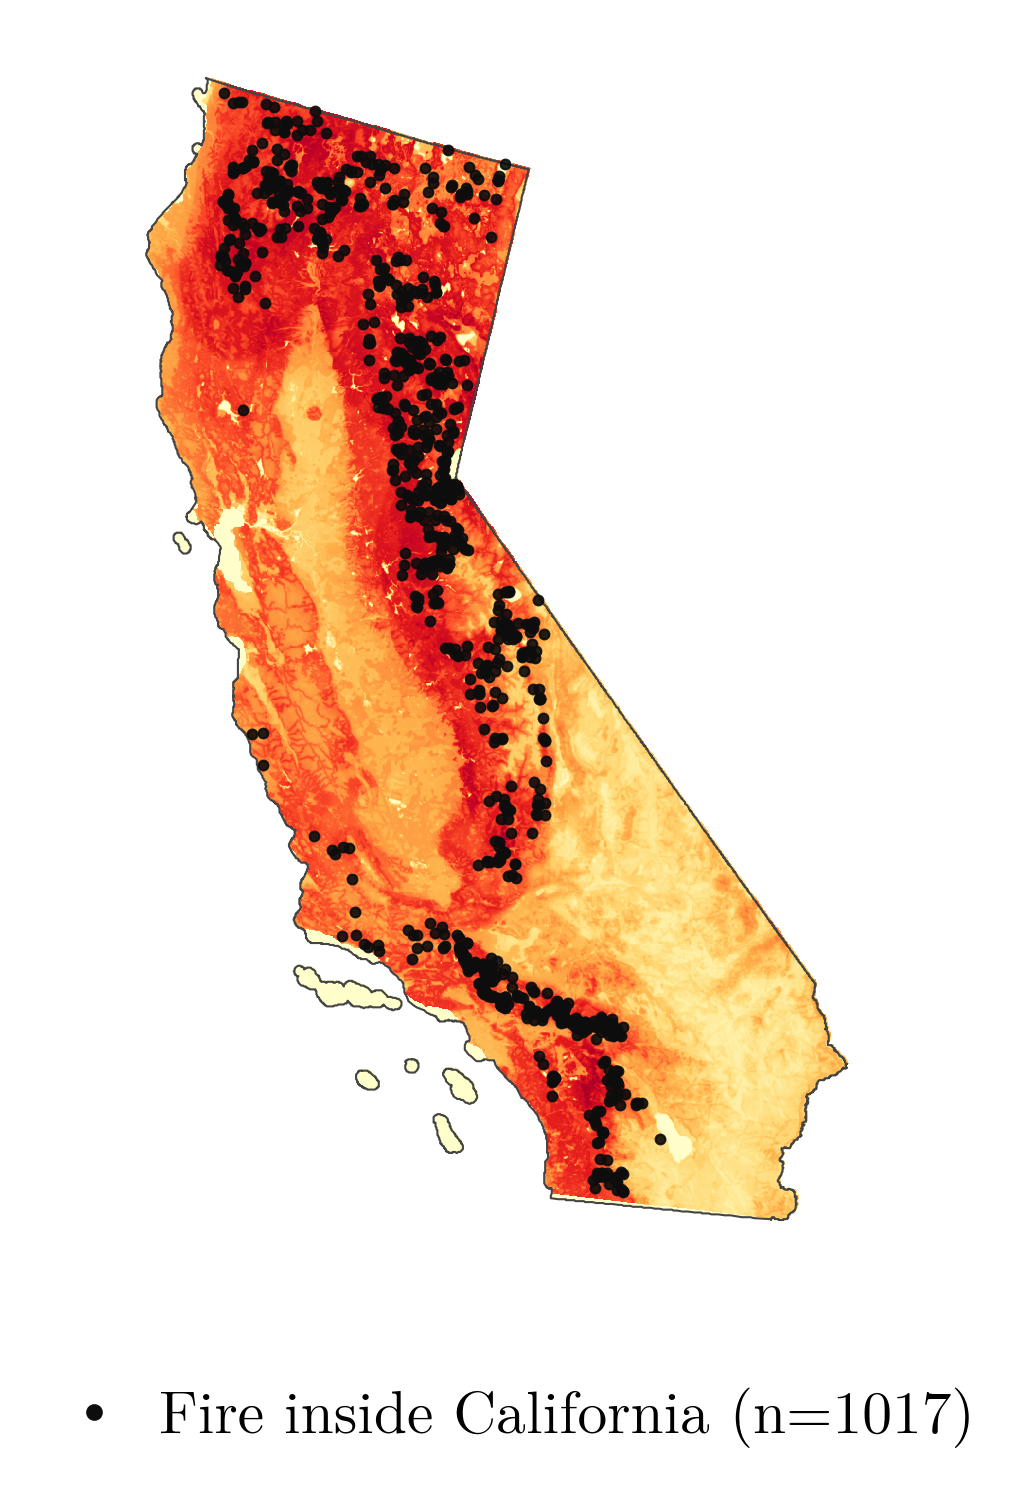
\includegraphics[width=\linewidth,height=0.31\textheight,keepaspectratio]{Figures/fig01_pyrologix_california_boundary.png}
        \caption{Study region}
        \label{fig:img1}
    \end{subfigure}
    \hfill
    \begin{subfigure}{0.48\textwidth}
        \centering
        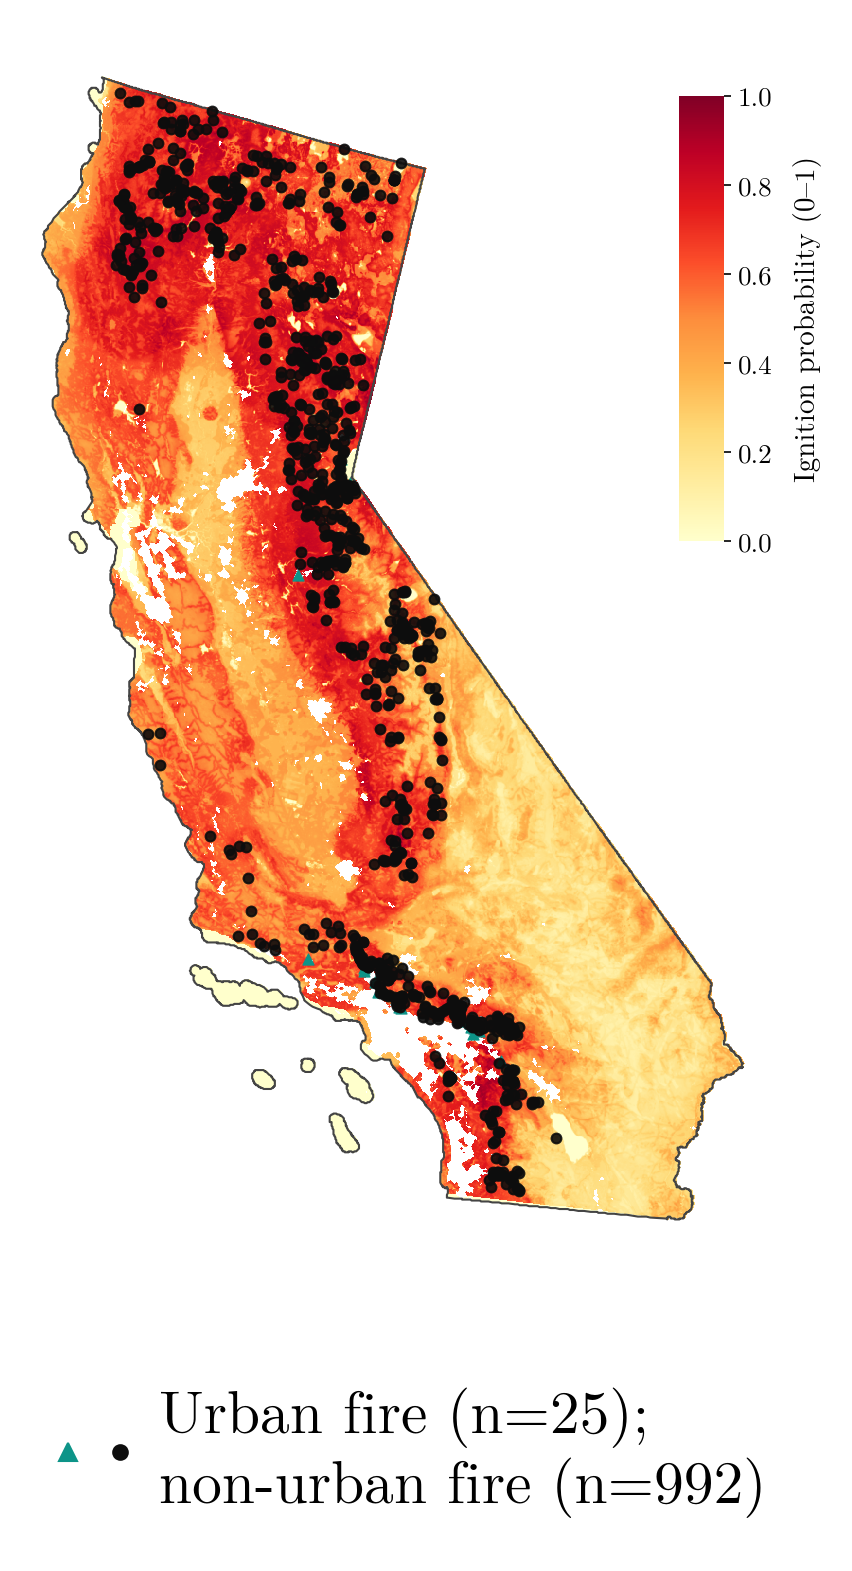
\includegraphics[width=\linewidth,height=0.31\textheight,keepaspectratio]{Figures/fig02_pyrologix_exclude_urban.png}
        \caption{Excluding urban areas}
        \label{fig:img2}
    \end{subfigure}

    \par\medskip

    % ----- Second row -----
    \begin{subfigure}{0.48\textwidth}
        \centering
        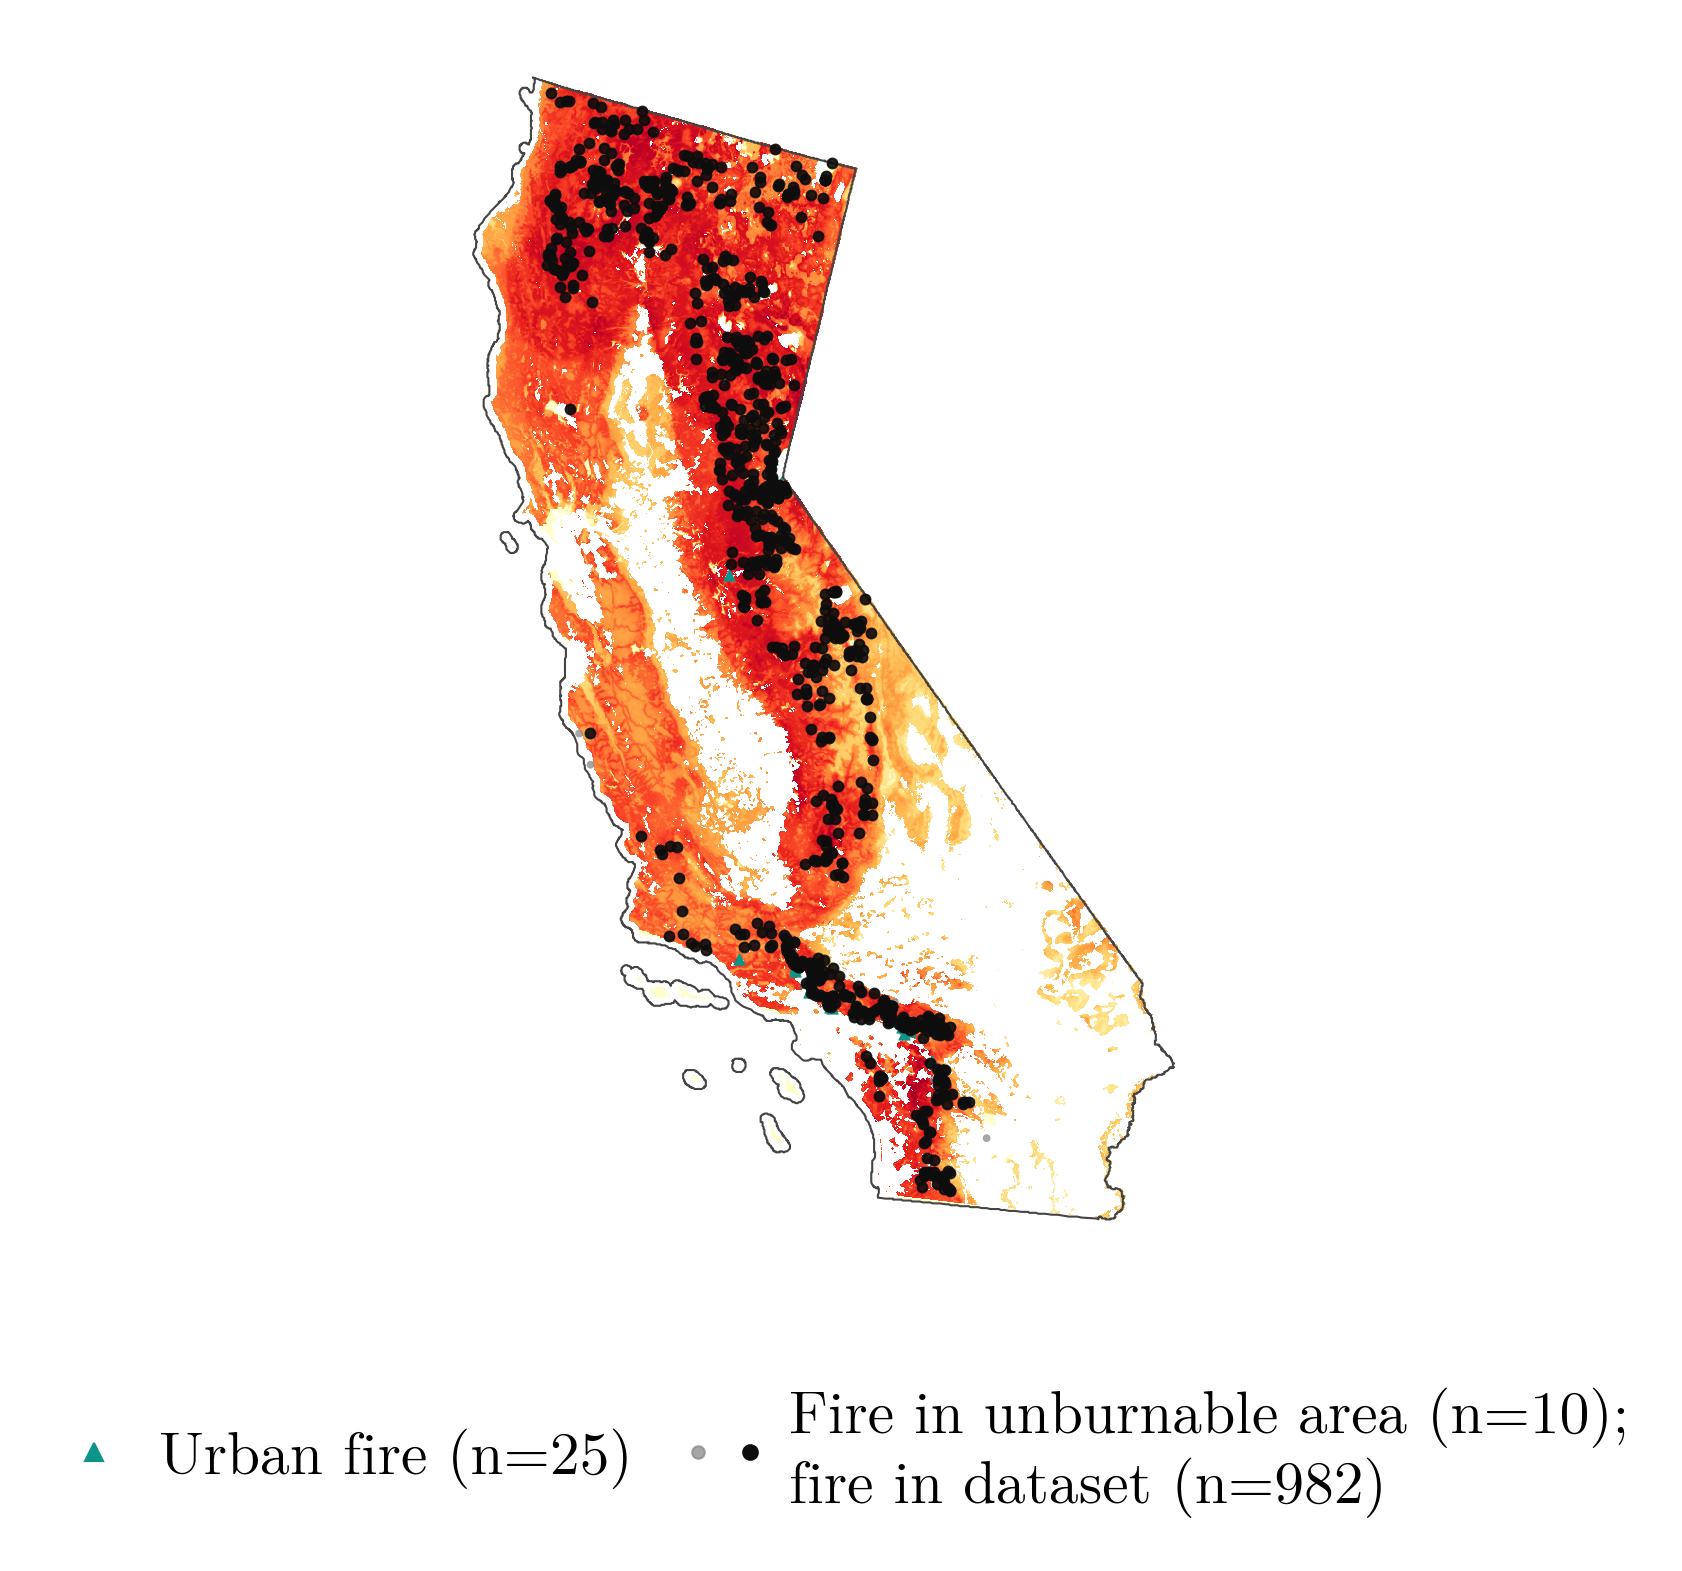
\includegraphics[width=\linewidth,height=0.31\textheight,keepaspectratio]{Figures/fig03_pyrologix_exclude_always_unburnable.png}
        \caption{{\small Excluding unburnable areas}}
        \label{fig:img4}
    \end{subfigure}
    \hfill
    \begin{subfigure}{0.48\textwidth}
        \centering
        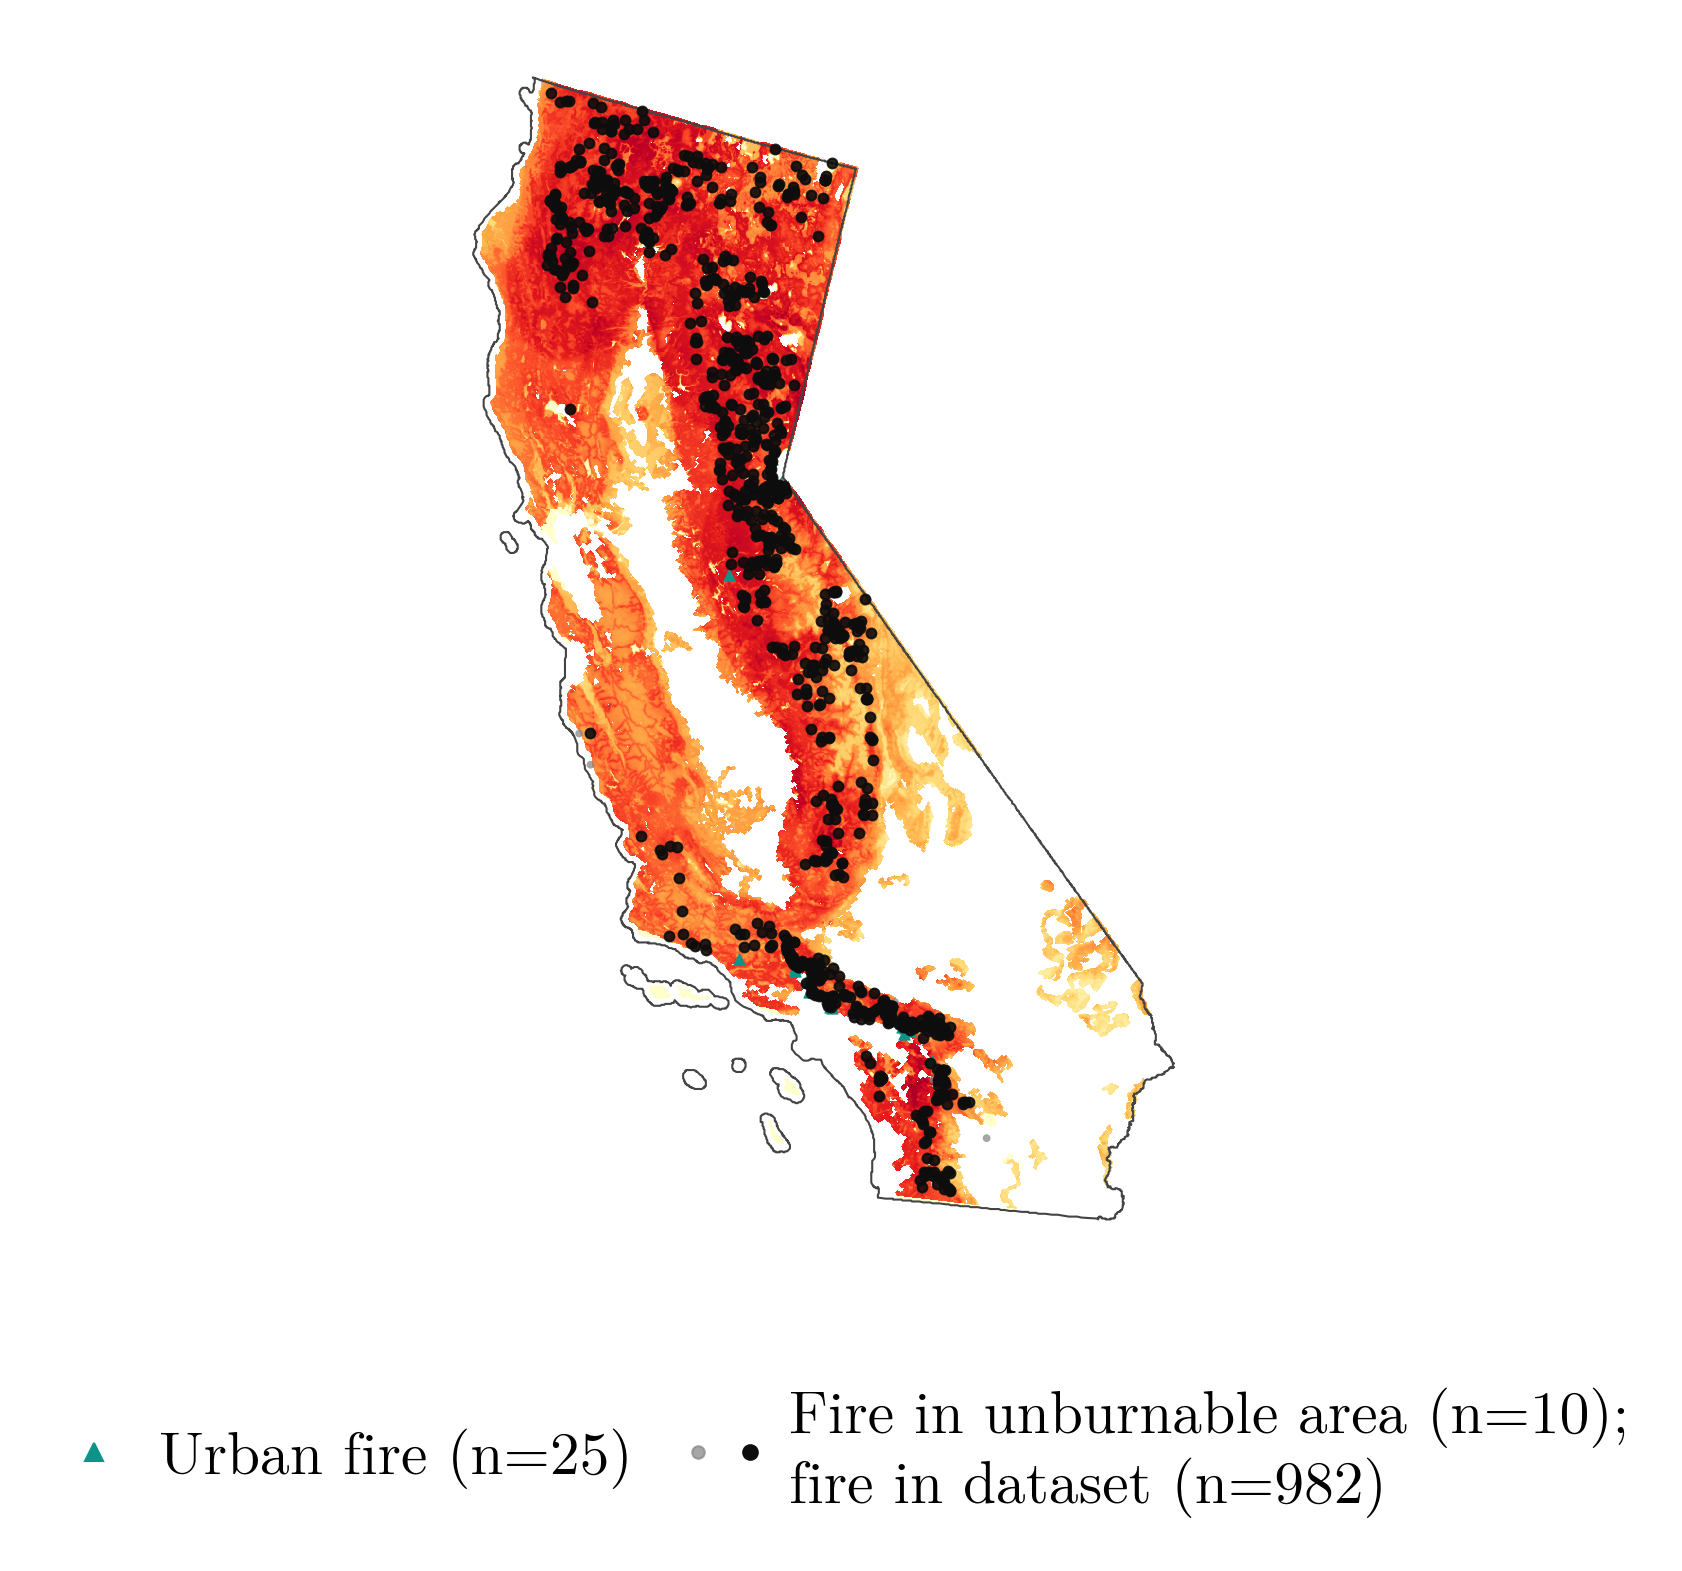
\includegraphics[width=\linewidth,height=0.31\textheight,keepaspectratio]{Figures/fig04_pyrologix_components_ge_9km2.png}
        \caption{{\small Filtering small isolated regions}.}
        \label{fig:img5}
    \end{subfigure}
    \caption{\textbf{California case study for wildfire monitoring.}
Sequential preprocessing of the study region used for the wildfire monitoring experiments.
\textbf{(a)}~Geographic overview of California with the wildfire risk map and historical ignition points.
\textbf{(b)}~Burnable landscape after excluding urban areas, with removed ignition points highlighted.
\textbf{(c)}~Further refinement after excluding permanently unburnable regions, such as water bodies, deserts, and barren land, with additionally excluded ignition points highlighted.
\textbf{(d)}~Final study region after removing unconnected burnable regions smaller than $9 \times 9$ km.}
    \label{fig:data}
\end{figure*}



To preserve ignition points near boundaries, a one-pixel buffer (9~km$^2$) is added around excluded areas. To avoid temporal leakage, we use the WFPI 2020 dataset rather than more recent releases.

% To avoid excluding historical wildfire ignitions that occur near the boundaries of these excluded regions, we add a one-pixel buffer (corresponding to 9~km$^2$) around all removed unburnable cells. This adjustment is motivated by observations from the USFS historical ignition dataset, in which several ignition points are located directly on boundaries that would otherwise be classified as unburnable. To prevent temporal data leakage between historical ignition records and the benchmark evaluation, we use the WFPI dataset from 2020 rather than more recent releases. 

\subsection*{Spatial-temporal grid construction}

The wildfire risk and historical ignition points data are provided on a projected equal-area grid at a spatial resolution of $d$ metres per cell and at an hourly temporal resolution. To make infrastructure placement and drone routing computationally tractable, we introduce a coarser \textit{operational grid} that aligns spatial and temporal scales with the physical capabilities of the monitoring hardware.

Each drone carries a sensor with detection radius $r$ metres, modelled as a square footprint of side $2r$ metres. We define the operational cell width $c = \mathrm{round}(2r/d)$ data cells, so that one operational cell corresponds to exactly one drone footprint. The data grid of $N_\mathrm{data} \times M_\mathrm{data}$ cells is tiled into non-overlapping $c \times c$ blocks, yielding an operational grid of
\[
N = \bigl\lfloor N_\mathrm{data}/c \bigr\rfloor \quad \text{and} \quad M = \bigl\lfloor M_\mathrm{data}/c \bigr\rfloor
\]
cells, on which all placement and routing decisions are made. The placement and routing models only act on this operational grid and do not consider the original data grid scale. A drone positioned at operational cell $(i,j)$ is assumed to observe the entire $c \times c$ block of data cells centred at that location. Planning at finer resolution would convey little additional operational information while scaling the decision problem quadratically.

The one-hour data timestep is both a constraint imposed by the temporal resolution of the historical ignition points data and a natural operational unit, since the drone battery capacity is set to one hour of flight time. A drone travelling at speed $v$ metres per minute can traverse
\[
k = \bigl\lfloor 60\,v / (c \cdot d) \bigr\rfloor
\]
operational cells per hour. Each such traversal constitutes one \textit{operational substep}, so a one-hour battery sustains exactly $k$ routing actions before requiring recharging. The simulation unfolds over hourly data timesteps, each subdivided into $k$ substeps during which drones move and fire detection is checked.

The wildfire risk map, originally at data resolution, is coarsened to the operational grid by averaging risk values within each $c \times c$ block. Each hourly risk value is then divided by $k$ and replicated $k$ times along the time axis, yielding per-substep risk values under the assumption of uniform ignition probability within each hour. All numerical parameter values used in the California case study are reported in Table~\ref{tab:benchmark_params}.



%%%%%%%%%%%%%%%%%%%%%


\subsection*{Infrastructure placement and drone allocation optimization}
% We formulate an optimization model that jointly determines the placement of ground sensing stations, the placement of charging stations, and the allocation of drones across charging stations in order to maximize wildfire monitoring coverage under a limited budget.
The notation used throughout this formulation is summarized in Table \ref{tab:infra_overview}.
% \small
% \begin{longtable}[h]{lll}
% \caption{Overview of sets, parameters, and decision variables used in the infrastructure placement optimization model.}
% \label{tab:infra_overview} \\
% \toprule
% \textbf{Sets} & \textbf{Description} & \textbf{Definition} \\
% \midrule
% \endfirsthead

% \multicolumn{3}{c}%
% {{\bfseries \tablename\ \thetable{} -- continued from previous page}} \\
% \toprule
% \textbf{Sets} & \textbf{Description} & \textbf{Definition} \\
% \midrule
% \endhead

% \midrule \multicolumn{3}{r}{{Continued on next page}} \\
% \endfoot

% \bottomrule
% \endlastfoot

% $\set I$ & Set of all grid points in the study region & $\{1,\dots,N\}\times\{1,\dots,M\}$ \\
% $\set I_{g}$ & Feasible grid points for ground sensors & $\subseteq \set I$ \\
% $\set I_{c}$ & Feasible grid points for charging stations & $\subseteq \set I$ \\

% \midrule
% \textbf{Parameters} & \multicolumn{2}{l}{\textbf{Description}} \\
% \midrule

% $r_{ij}$ & \multicolumn{2}{l}{Static wildfire risk score at grid point $(i,j)$} \\
% $c_g$ & \multicolumn{2}{l}{Cost of one ground sensing station} \\
% $c_c$ & \multicolumn{2}{l}{Cost of one charging station} \\
% $c_d$ & \multicolumn{2}{l}{Cost of one drone} \\
% $B$ & \multicolumn{2}{l}{Total deployment budget} \\
% $\bar n_D$ & \multicolumn{2}{l}{Maximum number of drones assignable to one charging station} \\
% $\epsilon$ & \multicolumn{2}{l}{Small regularization weight on infrastructure cost in the objective} \\
% $K_{uv}$ & \multicolumn{2}{l}{Uniform kernel coverage coefficient at relative offset $(u,v)$} \\
% $K_x$ & \multicolumn{2}{l}{Half-width of kernel support in the first grid dimension} \\
% $K_y$ & \multicolumn{2}{l}{Half-width of kernel support in the second grid dimension} \\

% \midrule
% \textbf{Variables} & \multicolumn{2}{l}{\textbf{Description}} \\
% \midrule

% $x^g_{ij} \in \{0,1\}$ & \multicolumn{2}{l}{1 if a ground sensing station is placed at grid point $(i,j)$} \\
% $x^c_{ij} \in \{0,1\}$ & \multicolumn{2}{l}{1 if denoting if a charging station is placed at grid point $(i,j)$} \\
% $n^c_{ij} \in \mathbb{Z}_+$ & \multicolumn{2}{l}{Denoting the number of drones allocated to charging station $(i,j)$} \\
% $\theta_{ij} \in \mathbb{R}$ & \multicolumn{2}{l}{Denoting infrastructure coverage level at grid point $(i,j)$} \\

% \end{longtable}
% \normalsize

\begin{table}[htbp]
\centering
\small
\caption{Overview of sets, parameters, and decision variables used in the infrastructure placement optimization model.}
\label{tab:infra_overview}
\begin{tabular}{lll}
\toprule
\textbf{Sets} & \textbf{Description} & \textbf{Definition} \\
\midrule
$\set I$ & Set of all grid points in the study region & $\{1,\dots,N\}\times\{1,\dots,M\}$ \\
$\set I_{g}$ & Feasible grid points for ground sensors & $\subseteq \set I$ \\
$\set I_{c}$ & Feasible grid points for charging stations & $\subseteq \set I$ \\
$\set P$ & Feasible (cell, station) pairs & $\subseteq \set I\times\set I_c$ \\

\midrule
\textbf{Parameters} & \multicolumn{2}{l}{\textbf{Description}} \\
\midrule
$r_{ij}$ & \multicolumn{2}{l}{Static wildfire risk score at grid point $(i,j)$} \\
$c_g$ & \multicolumn{2}{l}{Cost of one ground sensing station} \\
$c_c$ & \multicolumn{2}{l}{Cost of one charging station} \\
$c_d$ & \multicolumn{2}{l}{Cost of one drone} \\
$B$ & \multicolumn{2}{l}{Total deployment budget} \\
$\bar n_D$ & \multicolumn{2}{l}{Maximum number of drones assignable to one charging station} \\
$\epsilon$ & \multicolumn{2}{l}{Small regularization weight on infrastructure cost in the objective} \\
$\Delta_{s,k}$ & \multicolumn{2}{l}{Greedy incremental coverage fraction from the $k$-th drone at station $s$} \\

\midrule
\textbf{Variables} & \multicolumn{2}{l}{\textbf{Description}} \\
\midrule
$x^g_{ij} \in \{0,1\}$ & \multicolumn{2}{l}{1 if a ground sensing station is placed at grid point $(i,j)$} \\
$x^c_{ij} \in \{0,1\}$ & \multicolumn{2}{l}{1 if a charging station is placed at grid point $(i,j)$} \\
$z_{ij,k} \in \{0,1\}$ & \multicolumn{2}{l}{1 if charging station $(i,j)$ has at least $k$ drones, $k=1,\dots,\bar n_D$} \\
$u_{ij,s} \in \{0,1\}$ & \multicolumn{2}{l}{1 if cell $(i,j)$ is assigned to charging station $s$ for coverage} \\
$w_{ij,s} \in [0,1]$ & \multicolumn{2}{l}{Coverage fraction contributed by station $s$ to cell $(i,j)$} \\
$\theta_{ij} \in [0,1]$ & \multicolumn{2}{l}{Infrastructure coverage level at grid point $(i,j)$} \\
\bottomrule
\end{tabular}
\normalsize
\end{table}
\vspace{0.3cm}
\noindent \textit{Objective.} Given a budget, we jointly optimize the placement of ground sensors and charging stations, along with drone allocation, to maximize coverage of high-risk wildfire regions. Our objective is given by
\begin{align}
    \max_{\bm x^g,\bm x^c,\bm z,\bm u,\bm w,\bm \theta}\quad
& \sum_{(i,j)\in\mathcal I} r_{ij}\theta_{ij}
-\epsilon\left(
c_g\sum_{(i,j)\in\mathcal I_g} x^g_{ij}
+c_c\sum_{(i,j)\in\mathcal I_{\mathrm{c}}}x^c_{ij}
+c_d\sum_{(i,j)\in\mathcal I_{\mathrm{c}}}\sum_{k=1}^{\bar n_D}z_{ij,k}
\right).
\label{eq:infra_obj}
\end{align}
\noindent Here, we add a regularization term that ensures we avoid arbitrary over-deployment when the budget is nonbinding or weakly binding.\\
\\
\noindent \textit{Budget and resource allocation constraints.} These constraints are given by
\begin{align}
& c_g\sum_{(i,j)\in\mathcal I_g} x^g_{ij}
+c_c\sum_{(i,j)\in\mathcal I_c}x^c_{ij}
+c_d\sum_{(i,j)\in\mathcal I_c}\sum_{k=1}^{\bar n_D}z_{ij,k}
\le B,
\label{eq:infra_budget}\\
& z_{ij,k}\le x^c_{ij},
&&  (i,j)\in\mathcal I_c,\; k=1,\dots,\bar n_D,
\label{eq:infra_link_station}\\
& z_{ij,k}\ge z_{ij,k+1},
&&  (i,j)\in\mathcal I_c,\; k=1,\dots,\bar n_D-1.
\label{eq:infra_link_order}
\end{align}
Constraint \eqref{eq:infra_budget} enforces the overall deployment budget. Drone counts are encoded via ordered binary variables $z_{ij,k}$: constraint \eqref{eq:infra_link_station} ensures drones can only be allocated where a charging station is installed, and constraint \eqref{eq:infra_link_order} enforces the ordering so that $\sum_k z_{ij,k}$ correctly counts the number of drones at station $(i,j)$.\\
\\
\noindent \textit{Infrastructure siting constraint.} To prevent colocating both infrastructure types at the same feasible location, we impose
\begin{align}
& x^g_{ij}+x^c_{ij}\le 1,
&&  (i,j)\in\mathcal I_g \cap \mathcal I_c.
\label{eq:infra_exclusion}
\end{align}

\noindent \textit{Cell assignment and coverage constraints.}
The feasible set $\mathcal P \subseteq \mathcal I \times \mathcal I_c$ contains all (cell, station) pairs where the cell is reachable by a drone launched from the station within one battery charge, determined by breadth-first search on the masked operational grid. Each cell is assigned to at most one charging station:
\begin{align}
& \sum_{s:\,(i,j,s)\in\mathcal P} u_{ij,s}\le 1,
&&  (i,j)\in\mathcal I.
\label{eq:infra_assign}
\end{align}
The coverage fraction $w_{ij,s}$ that station $s$ contributes to cell $(i,j)$ is a piecewise-linear, diminishing-returns function of the drone count, precomputed with a greedy set-cover heuristic over drone patrol paths within the station's zone. For each additional drone level $k$, the heuristic selects the patrol path that maximises newly covered risk; the resulting incremental coverage fraction $\Delta_{s,k}$ is then applied uniformly to all reachable cells in the station's zone. This gives
\begin{align}
& w_{ij,s}\le \sum_{k=1}^{\bar n_D}\Delta_{s,k}\,z_{s,k},
&&  (i,j,s)\in\mathcal P,
\label{eq:infra_wbound_drone}\\
& w_{ij,s}\le u_{ij,s},
&&  (i,j,s)\in\mathcal P,
\label{eq:infra_wbound_assign}\\
& w_{ij,s}\ge 0,
&&  (i,j,s)\in\mathcal P.
\label{eq:infra_wpos}
\end{align}
Ground sensing stations provide direct local coverage at their installed grid cells. The overall coverage level at each cell combines ground sensing with drone-based surveillance:
\begin{align}
& \theta_{ij}\ge x^g_{ij},
&&  (i,j)\in\mathcal I_g,
\label{eq:infra_ground_only}\\
& \theta_{ij}\le x^g_{ij}+\sum_{s:\,(i,j,s)\in\mathcal P}w_{ij,s},
&&  (i,j)\in\mathcal I\cap\mathcal I_g,
\label{eq:infra_coverage_prime}\\
& \theta_{ij}\le \sum_{s:\,(i,j,s)\in\mathcal P}w_{ij,s},
&&  (i,j)\in\mathcal I\setminus\mathcal I_g.
\label{eq:infra_coverage_nonprime}
\end{align}
Constraints \eqref{eq:infra_coverage_prime}--\eqref{eq:infra_coverage_nonprime} combine direct sensing from ground stations with indirect drone-based coverage from charging stations.\\
\\
% Ground sensing stations provide direct local sensing at their installed grid cells. This is captured by constraints \eqref{eq:infra_ground_only}, which guarantee that any grid cell equipped with a ground sensor is immediately covered. Charging stations, however, contribute to coverage in a fundamentally different way. A charging station does not directly detect wildfire events itself; rather, it serves as the operational base from which drones are deployed. Because drones launched from a charging station can scan multiple nearby grid cells during their patrol, the monitoring influence of a charging station extends beyond its physical location. To represent this spatial operational reach, we model the coverage contribution of charging stations through a finite-support uniform kernel.
% More specifically, for each grid cell $(i,j)$, the model aggregates the contribution of charging stations located within a local neighborhood centered around that cell. The indices $dx$ and $dy$ denote relative spatial offsets in the horizontal and vertical grid directions, respectively. The kernel coefficients $K_{-dx,-dy}$ determine whether a charging station located at the shifted position $(i+dx,j+dy)$ contributes to the monitoring of the current cell. The use of a finite-support kernel reflects the fact that drones can only scan areas within a limited operational radius determined by battery capacity and local flight feasibility. Cells outside this neighborhood cannot be effectively monitored from the charging station and therefore contribute zero coverage. Because the kernel is uniform, all grid cells within this operational neighborhood contribute equally, which is consistent with the greedy uniform kernel station maximum coverage strategy implemented in the code.
% Importantly, the contribution from each charging station is scaled by the number of drones allocated to that station. Consequently, assigning more drones to a charging station proportionally increases its monitoring capability across its surrounding neighborhood, thereby coupling infrastructure placement decisions with drone resource allocation.
% Constraints \eqref{eq:infra_coverage_prime}--\eqref{eq:infra_coverage_nonprime} jointly define the spatial coverage induced by the deployed infrastructure, combining direct local sensing from ground stations with indirect multi-cell surveillance enabled by drones operating from charging stations.
\noindent \textit{Variable domain constraints.} Finally, the infrastructure decisions satisfy
\begin{align}
& 0\le \theta_{ij}\le 1,
&&  (i,j)\in\mathcal I,
\label{eq:infra_theta}\\
& x^g_{ij}\in\{0,1\},
&&  (i,j)\in\mathcal I_g,
\label{eq:infra_binary_g}\\
& x^c_{ij}\in\{0,1\},
&&  (i,j)\in\mathcal I_c,
\label{eq:infra_binary_c}\\
& z_{ij,k}\in\{0,1\},
&&  (i,j)\in\mathcal I_c,\; k=1,\dots,\bar n_D,
\label{eq:infra_binary_z}\\
& u_{ij,s}\in\{0,1\},
&&  (i,j,s)\in\mathcal P.
\label{eq:infra_binary_u}
\end{align}



%%%%%%%%%%%%%%%%%



\subsection*{Drone routing optimization}
% We propose three drone routing strategies: maximizing coverage (MaxCov) \cite{MCLPChurchRevelle}, the Team Orienteering Problem-based strategy (TOP) \cite{chao1996team}, and minimizing detection time (LinearMinTime), each capturing a different operational objective for wildfire monitoring. While the strategies share a common routing and feasibility structure, they differ in how surveillance performance is quantified and optimized. 
\blue{We propose three complementary drone-routing strategies for proactive wildfire monitoring: a Team Orienteering Problem-based strategy (TOP),  a maximum-coverage strategy (MaxCov), and a minimum-detection-time strategy (LinearMinTime). TOP builds on the classical Team Orienteering Problem introduced by Chao et al.~\cite{chao1996team}. MaxCov is adopted from~\cite{dronebench2025}, and builds on the classical maximal covering location problem introduced by Church and ReVelle~\cite{MCLPChurchRevelle}. LinearMinTime is introduced here to directly prioritize reduction of wildfire detection delay. While the strategies share a common routing and feasibility structure, they differ in how surveillance performance is quantified and optimized.}

We first summarize the sets, parameters, and decision variables of the routing models in Table~\ref{tab:routing_overview}. To restrict operations to accessible regions, we apply a binary spatial mask over the grid, excluding infeasible areas such as water bodies or terrain obstacles. A breadth-first search (BFS) from charging-station locations is then used to identify all reachable cells, defining the feasible set $\set I_d$. This ensures that routing is confined to connected, operationally feasible regions while reducing computational complexity.

\blue{In the rolling-horizon strategies (TOP and MaxCov), the wildfire risk map is updated between re-optimizations to reflect the mitigating effect of active monitoring. When a drone surveils a cell, that cell's accumulated ignition risk is reset to zero; while a cell remains unmonitored, its risk instead grows back linearly, accruing the cell's baseline per-step ignition probability $r_0$ at each step, so that after $k$ unmonitored steps its risk equals $k\,r_0$. This linear accumulation is the first-order Taylor approximation of the exact probability that at least one ignition has occurred over $k$ independent steps, $1-(1-r_0)^k = k\,r_0 + O\!\big((k r_0)^2\big)$, which is accurate here because per-cell hourly ignition probabilities are small. The minimum-detection-time strategy (LinearMinTime) does not modify the risk map explicitly; it instead encodes this same cumulative undetected risk directly in its objective.}

\begin{table}[htbp]
\centering
\small
\caption{Overview of sets, parameters, and decision variables used in the drone routing optimization models. The max-coverage and min-detection-time formulations share a common time-indexed structure, while the TOP formulation optimizes routes directly on a routing graph.}
\label{tab:routing_overview}
\begin{tabular}{lll}
\toprule
\textbf{Sets} & \textbf{Description} & \textbf{Definition} \\
\midrule
$\mathcal T$ & Set of time periods in the optimization horizon & $\{1,\dots,T\}$ \\
$\mathcal S$ & Set of drones & $\{1,\dots,S\}$ \\
$\mathcal C$ & Set of charging stations & $\{1,\dots,C\}$ \\
$\mathcal I_d$ & Set of feasible grid cells for drone movement & $\subseteq \mathcal I$ \\
$\mathcal I_{\mathrm{det}}$ & Set of detectable grid cells & $\subseteq \mathcal I_d$ \\
$\mathcal N(i)$ & Set of feasible neighboring cells of cell $i$ & $\subseteq \mathcal I_d$ \\
$\mathcal V$ & Routing graph nodes (TOP) & $\mathcal I_{\mathrm{det}} \cup \{o,e\}$ \\
\midrule
\textbf{Parameters} & \multicolumn{2}{l}{\textbf{Description}} \\
\midrule
$r_{t+\delta,i}$ & \multicolumn{2}{l}{Wildfire risk at cell $i$ at global time $t+\delta$} \\
$B_{\max}$ & \multicolumn{2}{l}{Maximum drone battery capacity} \\
$\Delta_i$ & \multicolumn{2}{l}{Shortest path distance to nearest charging station} \\
$\bar C$ & \multicolumn{2}{l}{Charging-station capacity} \\
$T$ & \multicolumn{2}{l}{Optimization horizon length} \\
$\delta$ & \multicolumn{2}{l}{Time offset} \\
$T_{\mathrm{reev}}$ & \multicolumn{2}{l}{Number of periods executed before re-optimization} \\
$\ell(j)$ & \multicolumn{2}{l}{Grid cell associated with charging station $j$} \\
$c_{ij}$ & \multicolumn{2}{l}{Travel cost between nodes $i$ and $j$ (TOP)} \\
% $L$ & \multicolumn{2}{l}{Maximum route length / battery budget (TOP)} \\
$o$ & Origin depot (TOP) \\ 
$e$ & End depot (TOP) \\
\midrule
\textbf{Decision variables} & \multicolumn{2}{l}{\textbf{Description}} \\
\midrule
$a_{its}\in\{0,1\}$ & \multicolumn{2}{l}{Drone $s$ at grid cell $i$ at time $t$} \\
$c_{jts}\in\{0,1\}$ & \multicolumn{2}{l}{Drone $s$ charging at station $j$ at time $t$} \\
$b_{ts}\in\mathbb Z_+$ & \multicolumn{2}{l}{Battery level} \\
$\theta_{ti}\in\{0,1\}$ & \multicolumn{2}{l}{Coverage variable (max coverage)} \\
$\zeta_{it}\in\mathbb Z_+$ & \multicolumn{2}{l}{Visit-history variable (min detection time)} \\
$w_{itt'}\in\{0,1\}$ & \multicolumn{2}{l}{Undetected risk indicator} \\
$y_{is}\in\{0,1\}$ & \multicolumn{2}{l}{Drone $s$ visits node $i$ (TOP)} \\
$x_{ijs}\in\{0,1\}$ & \multicolumn{2}{l}{Drone $s$ traverses arc $(i,j)$ (TOP)} \\
\bottomrule
\end{tabular}
\normalsize
\end{table}
% Our objective is to minimize the expected wildfire detection time. The detection time is defined as the elapsed time between wildfire ignition and first detection by any monitoring device. For example, if a fire ignites at time \(t_0 = 3\) and is detected at time \(t_d = 6\), then the detection time is \(\Delta t = t_d - t_0 = 3\).
% % , that is, the expected time until a fire is first detected by any monitoring device. 
% Importantly, the detection time \(\Delta t\) is itself a random variable, as it depends on both the randomness associated with the wildfire ignitions and the operational decisions, including sensor placement and drone routing. Writing this objective exactly leads to a highly nonlinear stochastic integer program, since the probability of detection at time \(t\) depends on the full sequence of prior visits to the cell as well as the cumulative probability that ignition has occurred since the most recent visit.

% To obtain a computationally tractable formulation, we construct a linear approximation of the objective function. Instead of directly minimizing the expected detection time, we minimize the total cumulative probability risk, defined as the cumulative probability that a given cell is burning between successive visits. This provides a natural surrogate for expected detection delay: the longer a high-risk cell remains unvisited, the larger the probability mass that accumulates over time. Consequently, minimizing cumulative undetected risk promotes earlier and more frequent surveillance of high-risk regions.

% This approximation is motivated by the fact that the expected detection time can be expressed as the sum over time of the probabilities that a wildfire remains undetected up to each period. Therefore, minimizing the cumulative probability that cells are burning between visits serves as a tractable proxy for minimizing the expected wildfire detection time.
\subsubsection*{Team Orienteering Problem (TOP)}

\noindent \textit{Objective.}
\blue{The Team Orienteering Problem (TOP) strategy formulates wildfire monitoring as a route-selection problem in which drones seek to maximize the cumulative wildfire risk observed within a finite battery horizon. Each drone departs from a charging station, visits a subset of feasible grid cells, and must return to a charging station before battery depletion.}  The objective is given by
\begin{equation}
\label{eq:top_obj}
\max \quad
\sum_{s \in \mathcal{S}}
\sum_{i \in \mathcal{I}_{\mathrm{d}}}
r_i y_{is}.
\end{equation}
\blue{Unlike time-indexed routing formulations, TOP optimizes complete drone routes directly on a routing graph rather than sequential drone positions over time.}\\
\\
% \noindent \textit{Objective.} 
% % \danique{Mention here also that the difference between max coverage and TOP is that max coverage can handle dynamics much better, as we can update the riskmap every re-evaluation step, while for TOP we can do it only after each battery cycle.}
% % The objective is to construct a complete route for each drone over a finite battery horizon such that the total wildfire risk collected by the fleet is maximized. In contrast to the minimizing detection time and maximum coverage models, which explicitly track drone positions over time, the Team Orienteering Problem (TOP) formulation optimizes complete paths directly on a routing graph.
% The objective is to maximize collected wildfire risk via complete drone routes over a finite horizon. Unlike other models, TOP optimizes paths directly on a routing graph. The objective is given by
% \begin{equation}
% \label{eq:top_obj}
% \max \quad
% \sum_{s \in \mathcal{S}}
% \sum_{i \in \mathcal{I}_{\mathrm{d}}}
% r_i y_{is}.
% \end{equation}
\noindent \textit{Artificial origin and destination depots.}
The artificial depot nodes, $o$ and $e$, correspond to the same physical charging station, but  are modeled as distinct nodes to separate departure and return flows, a standard approach in vehicle-routing formulations.\\
\\
% For example, instead of writing a route as
% $
% c \rightarrow i_1 \rightarrow i_2 \rightarrow c,
% $
% where $c$ is the charging station, we equivalently write
% $
% o \rightarrow i_1 \rightarrow i_2 \rightarrow d.
% $
% This allows route-start and route-end constraints to be expressed more clearly and prevents degenerate cycles at the charging station.\\
% \\
\noindent \textit{Routing constraints.}
The constraints are given by
\begin{align}
& \sum_{s \in \mathcal{S}} y_{is} \le 1,
&& i \in \mathcal{I}_{\mathrm{d}},
\label{eq:top_unique_visit}
\\
& \sum_{j \in \mathcal{V}^{-}} x_{ojs} = 1,
&& s \in \mathcal{S},
\label{eq:top_start}
\\
& \sum_{i \in \mathcal{V}^{+}} x_{ies} = 1,
&& s \in \mathcal{S},
\label{eq:top_end}
\\
& x_{jos}=0,
&& j \in \mathcal{V},\ s \in \mathcal{S},
\label{eq:top_no_enter_origin}
\\
& x_{ejs}=0,
&& j \in \mathcal{V},\ s \in \mathcal{S},
\label{eq:top_no_leave_dest}
\\
& \sum_{j \in \mathcal{V}^{-}\setminus\{i\}} x_{ijs}
=
y_{is},
&& i \in \mathcal{I}_{\mathrm{d}},\ s \in \mathcal{S},
\label{eq:top_outflow}
\\
& \sum_{j \in \mathcal{V}^{+}\setminus\{i\}} x_{jis}
=
y_{is},
&& i \in \mathcal{I}_{\mathrm{d}},\ s \in \mathcal{S},
\label{eq:top_inflow}
\end{align}
where $\mathcal{V}=\mathcal{I}_{\mathrm{d}}\cup\{o,e\}$, $\mathcal{V}^{+}=\mathcal{I}_{\mathrm{d}}\cup\{o\}$, and $\mathcal{V}^{-}=\mathcal{I}_{\mathrm{d}}\cup\{e\}$.

Constraints \eqref{eq:top_unique_visit} ensure that each grid point is served by at most one drone, thereby avoiding duplicate reward collection across the fleet. Constraints \eqref{eq:top_start} and \eqref{eq:top_end} ensure that each drone departs from the charging station and returns exactly once. Constraints \eqref{eq:top_outflow} and \eqref{eq:top_inflow} ensure that if a cell is visited, it must be entered and exited exactly once.\\
\\
\noindent \textit{Battery and travel constraints.}
The battery feasibility constraints are given by
\begin{align}
& \sum_{i \in \mathcal{V}^{+}}
\sum_{\substack{j \in \mathcal{V}^{-}\\ j \neq i}}
c_{ij}x_{ijs}
\le B_{\text{max}},
&& s \in \mathcal{S},
\label{eq:top_battery}
\end{align}
\noindent ensuring that the total travel distance of each drone remains within the battery capacity $B_{\text{max}}$. The travel cost $c_{ij}$ is defined using the $L_{\infty}$ metric.
% such that adjacent horizontal, vertical, and diagonal moves incur unit cost, while non-adjacent moves are assigned a prohibitive cost, thereby restricting routing to local neighbor transitions. 
% . Consequently, the routing graph only permits local movement between neighboring cells, which is consistent with the drone movement assumptions used in the time-indexed routing formulations.
\\
\\
\textit{Symmetry-breaking constraints.} Constraints \eqref{eq:top_symmetry} improve computational efficiency by reducing equivalent solutions that differ only by permutation of drone labels.
% are symmetry-breaking constraints, ordering drones by decreasing collected wildfire risk. This improves computational efficiency 
% by reducing equivalent solutions that differ only by permutation of drone labels.
\begin{align}
    & \sum_{i \in \mathcal{I}_{\mathrm{d}}} r_i y_{i,s+1}
\le
\sum_{i \in \mathcal{I}_{\mathrm{d}}} r_i y_{is},
&& s=1,\dots,|\mathcal{S}|-1.
\label{eq:top_symmetry}
\end{align}
\\
\\
\noindent \textit{Particle swarm optimization (PSO) routing heuristic.}
The TOP formulation yields a large combinatorial problem whose complexity scales rapidly with the number of drones, grid cells, charging stations, and arcs, making exact optimization intractable for large or time-sensitive wildfire applications. We therefore adopt the PSO heuristic in~\cite{PSO} to efficiently explore candidate multi-drone routes and obtain high-quality solutions at lower cost. The reported TOP-based routing results in Table~\ref{tab:detection} are thus heuristic. We adapt this algorithm to our grid structure to make it substantially faster, principally through a sparse split procedure that exploits the small number of charging stations, conservative filtering of local-search moves that cannot change the solution, and incremental route updates; Appendix~\ref{app:pso} details these changes, and the implementation is available in the code released with this paper (see the Code Availability statement).

\subsubsection*{Maximizing coverage}
\blue{We adopt the risk-aware maximum-coverage drone routing strategy developed in \cite{dronebench2025}. Drone routing is performed using a rolling-horizon optimization approach, in which a mixed-integer linear program is repeatedly solved over a finite planning horizon while only the decisions for a short implementation window are executed before re-optimization. The problem is subsequently re-solved using updated drone locations, battery states, and monitoring information, allowing the system to continuously adapt surveillance as operations evolve.}

\blue{At each optimization step, drones are routed to prioritize surveillance of high-risk regions by maximizing the cumulative wildfire risk of newly monitored areas within the planning horizon. The optimization accounts for operational constraints including battery endurance, charging requirements, charging-station capacities, communication limits, feasible movement between neighboring locations, and safe return feasibility to prevent battery depletion. Repeated surveillance of recently monitored regions is discounted to encourage spatial exploration and improve large-scale coverage. Full methodological details are provided in \cite{dronebench2025}.}



% In the present max-coverage setting, the wildfire risk map is static over time. However, the rolling-horizon framework readily generalizes to dynamic settings in which wildfire risk estimates are updated over time, since newly available information can be incorporated at each reevaluation step prior to reoptimization. Moreover, by decomposing the full operational problem into a sequence of smaller finite-horizon optimization problems, this approach significantly improves computational tractability.

% \begin{figure*}[!tb]
%     \centering
%     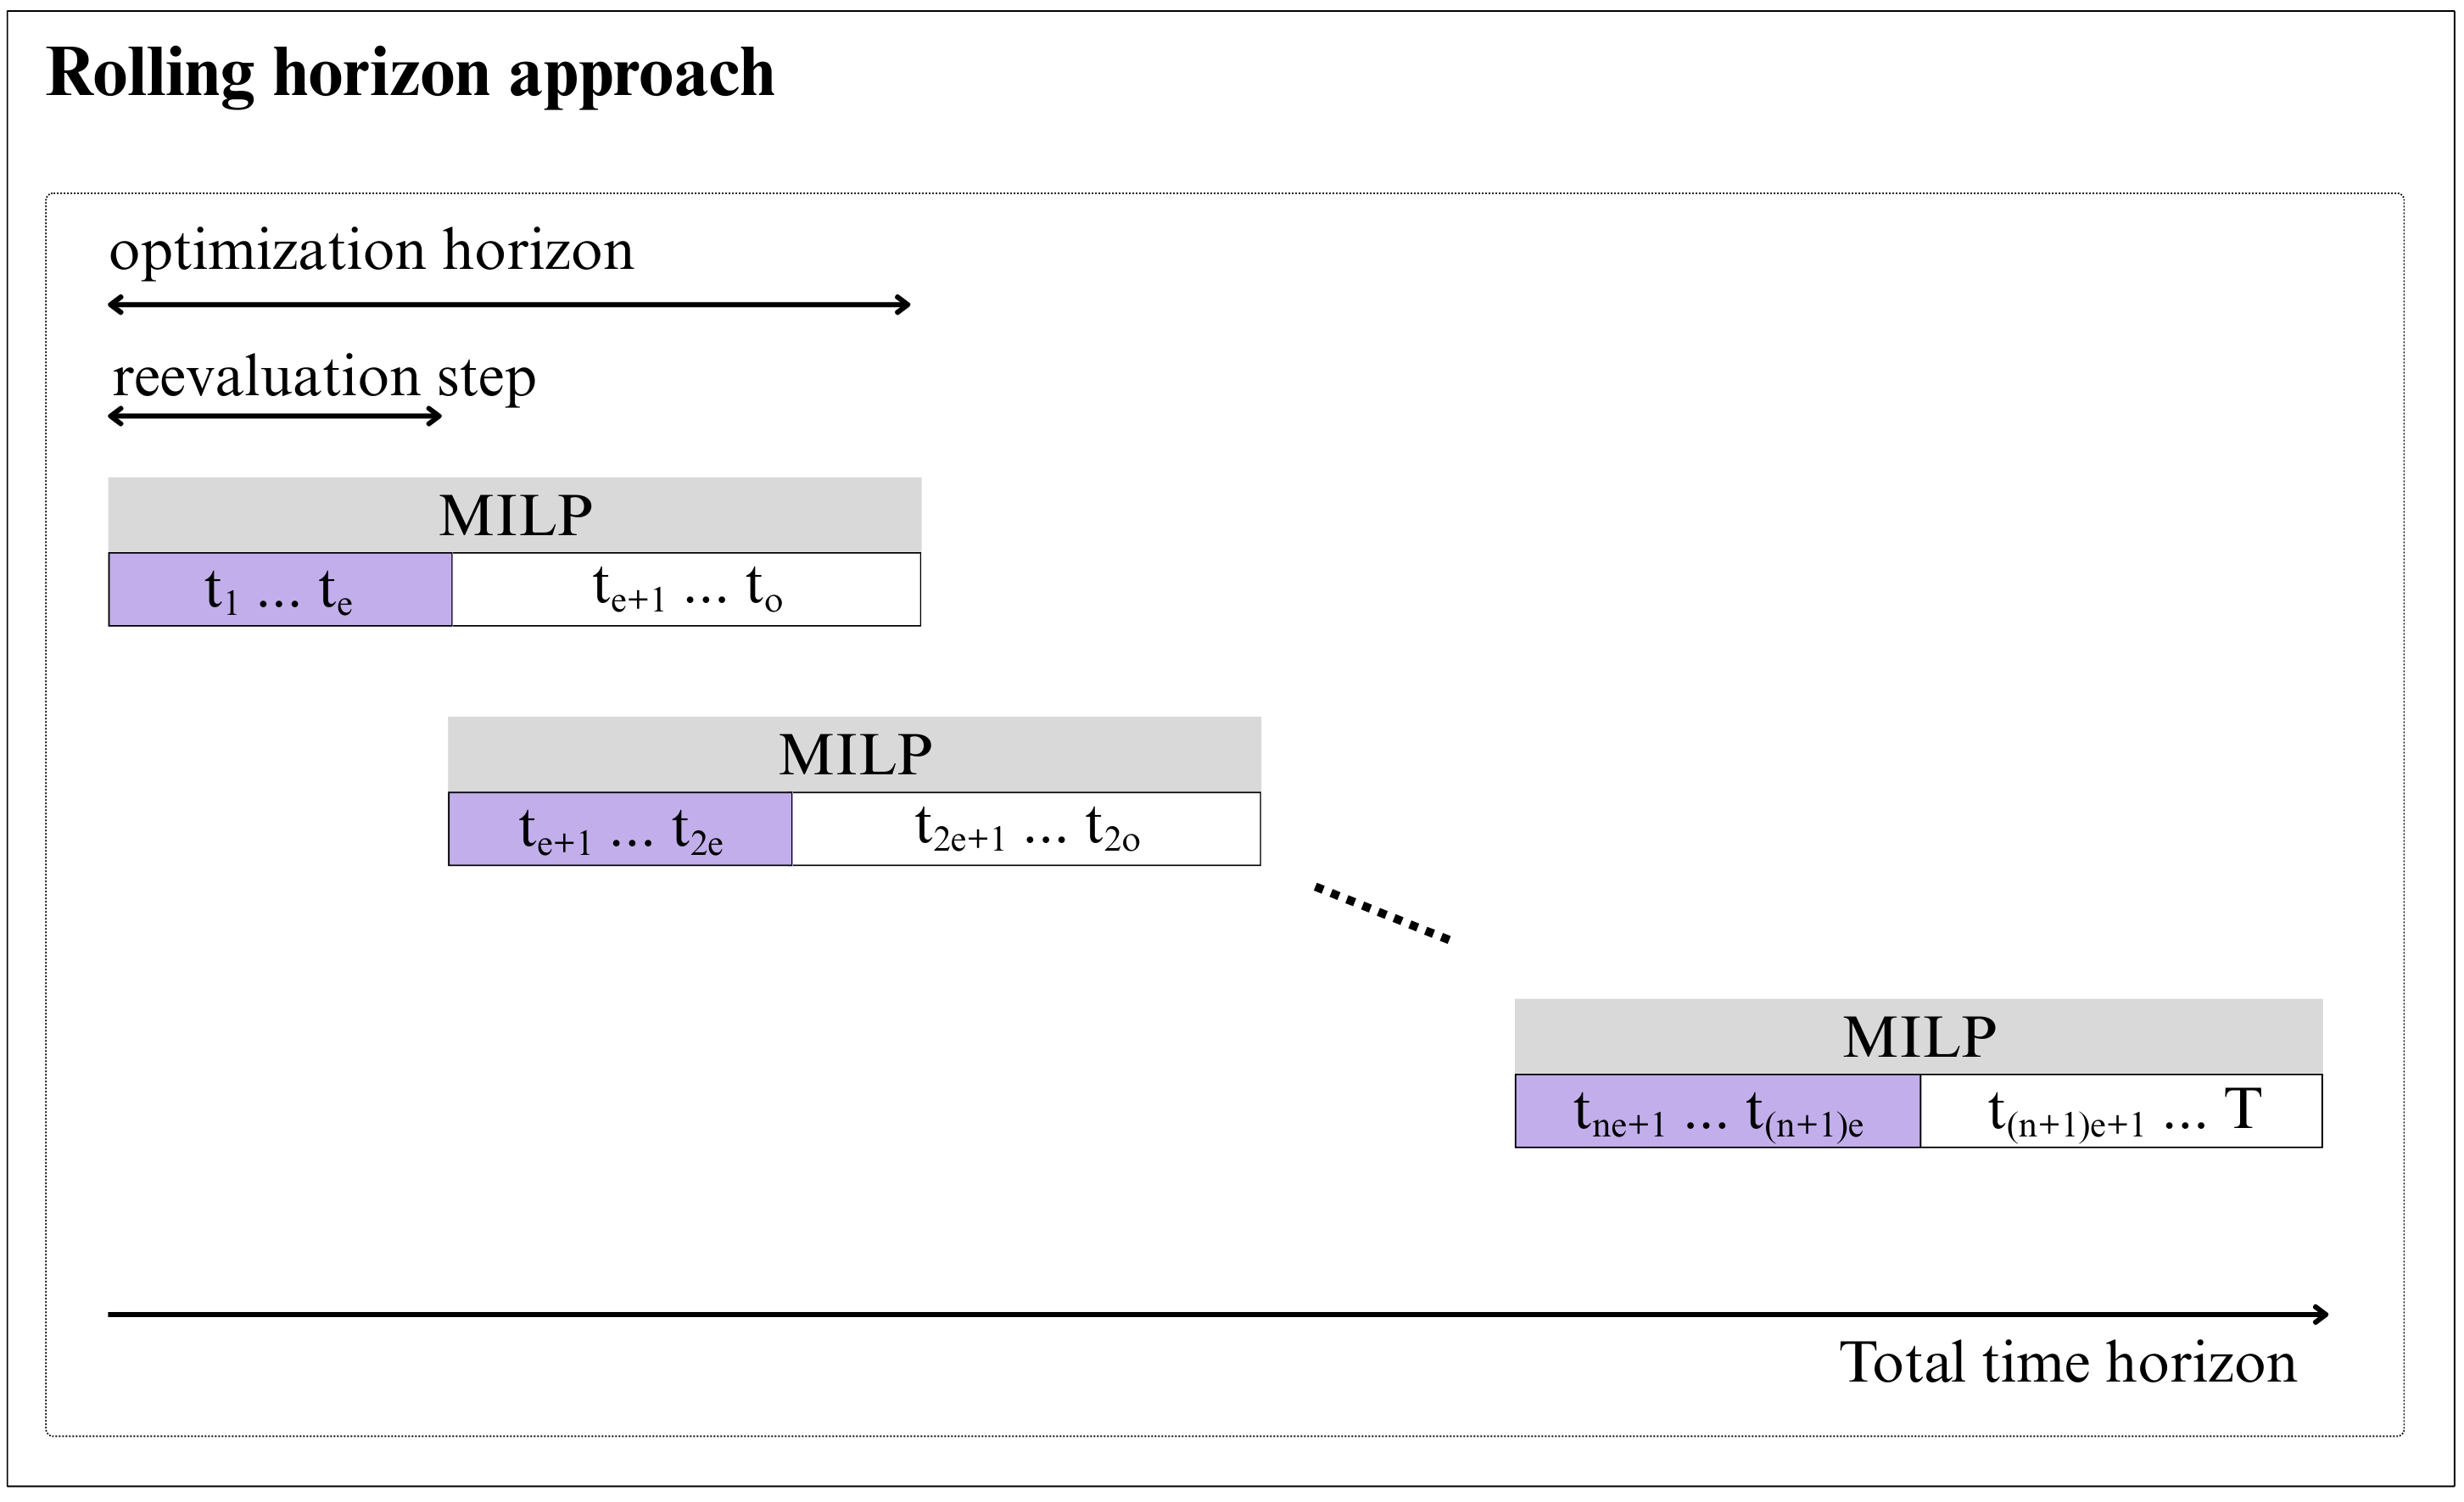
\includegraphics[width=\linewidth,height=0.42\textheight,keepaspectratio]{Figures/rollinghorizon.png}
%     \caption{The rolling horizon optimization framework. The problem is solved over an optimization horizon of $T$ time steps (the purple + white block) using Mixed Integer Linear Programming (MILP). Even though solutions are generated for $T$ time steps, we only use the $T_{\text{reev}}$ first ones (depicted in purple). After each reevaluation step, the horizon is shifted forward, and the problem is solved again. This process continues until the end of the total time horizon is reached, ensuring adaptability to new information and improved solution quality over time.}
%     \label{fig:rollinghorizon}
% \end{figure*}
% \vspace{0.3cm}
% \noindent \textit{Objective.}  
% The model maximizes the cumulative wildfire risk of grid cells visited for the first time within the planning horizon:
% \begin{align}
% \max_{\bm a,\bm c,\bm b,\bm \theta}\quad
% & \sum_{i\in\mathcal I_{\mathrm{d}}} r_{1+\delta,i}\,\theta_{1i}
% + \sum_{t=2}^{T}\sum_{i\in\mathcal I_{\mathrm{d}}} r_{t+\delta,i}\bigl(\theta_{ti}-\theta_{t-1,i}\bigr).
% \end{align}
% Here, $\delta$ denotes the current global time offset in the rolling-horizon implementation, linking the local optimization horizon to the full time horizon. The objective rewards only newly covered cells, so revisiting previously observed locations does not increase the objective value.\\
% \\
% To align the current optimization horizon with the total operational timeline, we introduce an offset parameter $\delta$, which denotes the current global time index at which the routing problem is solved. Consequently, the wildfire risk at local optimization time $t\in\mathcal T$ is evaluated using the global risk value $r_{t+\delta,i}$ for each detectable grid cell $i\in\mathcal I_{\mathrm{det}}$. 

% Before formulating the drone routing optimization model, we first define the feasible operational region over which drones are allowed to move. To ensure that drones operate only over physically accessible areas, we introduce a binary spatial mask over the study grid, where masked-out cells represent inaccessible regions, such as terrain obstacles, water bodies, or areas excluded from surveillance. 

% The feasible drone grid $\mathcal I_d$ is defined as the set of all admissible grid cells that are reachable from at least one charging station. To construct this connected operational region, we use a breadth-first search (BFS) procedure over the adjacency structure of the masked grid. Starting from the charging-station locations, BFS recursively explores all adjacent admissible cells and expands until all reachable cells have been identified. For each cell $i\in\mathcal I_d$, we denote by $\mathcal N(i)$ the set of feasible neighboring cells that can be reached in a single time step. As a result, inaccessible or disconnected cells are excluded from the routing model, ensuring that all optimized drone paths remain operationally feasible while improving computational tractability.\\
% \\
% \noindent \textit{Objective.}  
% At each optimization step, the routing model seeks to maximize the cumulative wildfire risk associated with grid cells that are visited for the first time within the planning horizon. The objective is given by
% \begin{align}
% \max_{\bm a,\bm c,\bm b,\bm \theta}\quad
% & \sum_{i\in\mathcal I_{\mathrm{det}}} r_{1+\delta,i}\,\theta_{1i}
% + \sum_{t=2}^{T}\sum_{i\in\mathcal I_{\mathrm{det}}} r_{t+\delta,i}\bigl(\theta_{ti}-\theta_{t-1,i}\bigr).
% \label{eq:routing_obj}
% \end{align}
% Here, \(\delta\) denotes the current time offset in the receding-horizon implementation. The objective rewards only newly covered cells, since a cell contributes at time \(t\) only through the increment \(\theta_{ti}-\theta_{t-1,i}\). As a result, revisiting a cell that has already been covered does not generate additional objective value.\\
% \\
% \noindent \textit{State and movement constraints.}  
% These constraints ensure that each drone occupies exactly one grid point at each time period and moves only along feasible neighbors:
% \begin{align}
% & \sum_{i\in\mathcal I_d} a_{its}
% + \sum_{j\in\mathcal C} c_{jts}
% = 1,
% && t\in\mathcal T,\ s\in\mathcal S,
% \label{eq:routing_state}\\
% & c_{j,t+1,s}+a_{\ell(j),t+1,s}
% \le
% \sum_{i\in\mathcal N(\ell(j))} a_{its}+c_{jts},
% && j\in\mathcal C,\ t=1,\dots,T-1,\ s\in\mathcal S,
% \label{eq:routing_move_charge}\\
% & a_{i,t+1,s}
% \le
% \sum_{i'\in\mathcal N(i)} a_{i'ts},
% && i\in\mathcal I_d\setminus\mathcal C,\ t=1,\dots,T-1,\ s\in\mathcal S.
% \label{eq:routing_move_fly}
% \end{align}
% % Constraint \eqref{eq:routing_state} enforces that each drone is either flying at one feasible grid point or charging at one charging station in every period. Constraint \eqref{eq:routing_move_charge} governs transitions into charging-station cells: a drone may charge at station \(j\) or fly at the corresponding charging-station cell \(\ell(j)\) at time \(t+1\) only if it was either charging there at time \(t\) or arrived from a neighboring feasible cell. Constraints \eqref{eq:routing_move_fly} govern drone movement to non-charging cells and ensures that drones transition only between feasible neighboring grid cells. To define the set of feasible drone locations, we construct the reachable surveillance region as the set of grid cells that can be connected to at least one charging station through a sequence of feasible movements. This reachable region is obtained using a breadth-first search (BFS) procedure over the grid adjacency structure.
% Constraints \eqref{eq:routing_state} enforce that, at each time period, every drone is in exactly one operational state: either flying at a feasible grid cell or charging at a charging station. Constraints \eqref{eq:routing_move_charge} govern movements involving charging stations. In particular, a drone may remain charging at station $j$ or move to the grid cell associated with that station at time $t+1$ only if it was already charging there at time $t$ or arrived from a neighboring feasible cell. Constraints \eqref{eq:routing_move_fly} govern movements between non-charging grid cells and ensure that drones move only between feasible neighboring cells.\\
% \\
% % To ensure that drones operate only over physically accessible regions, we first define a binary spatial mask over the study grid, where masked-out cells represent inaccessible areas, such as terrain obstacles, water bodies, or regions excluded from surveillance. Two cells are considered feasible neighbors only if they are adjacent and both belong to the admissible masked region. The feasible drone grid $\mathcal I_d$ is then constructed as the set of all masked cells that are reachable from at least one charging station. To determine this connected operational region, we use a breadth-first search (BFS) procedure over the adjacency structure of the masked grid. BFS systematically explores all neighboring cells starting from the charging-station locations and recursively expands to all connected feasible cells. This construction ensures that inaccessible or disconnected cells are excluded from the routing model, so all optimized drone paths remain operationally feasible. In addition, restricting the optimization problem to the connected reachable region improves computational tractability by avoiding unnecessary variables and constraints over irrelevant parts of the grid.
% \noindent \textit{Battery constraints.}  
% Drone operation is limited by battery endurance and the requirement that each drone must be able to return to a charging station:
% \begin{align}
% & 0 \le b_{ts} \le B_{\max},
% && t\in\mathcal T,\ s\in\mathcal S,
% \label{eq:routing_battery_bounds}\\
% & b_{ts}\ge B_{\max}\sum_{j\in\mathcal C} c_{jts},
% && t\in\mathcal T,\ s\in\mathcal S,
% \label{eq:routing_battery_charge}\\
% & b_{t+1,s}\le b_{ts}-1+(B_{\max}+1)\sum_{j\in\mathcal C} c_{j,t+1,s},
% && t=1,\dots,T-1,\ s\in\mathcal S,
% \label{eq:routing_battery_dyn}\\
% & b_{Ts}\ge \Delta_i\,a_{iTs},
% && i\in\mathcal I_d,\ s\in\mathcal S.
% \label{eq:routing_return}
% \end{align}
% Constraints \eqref{eq:routing_battery_bounds} bound the battery level of each drone between zero and its maximum capacity. Constraint \eqref{eq:routing_battery_charge} ensures that a drone located at a charging station is restored to full battery capacity. Constraint \eqref{eq:routing_battery_dyn} models the battery evolution over time, accounting for one unit of battery consumption during flight and battery replenishment when charging occurs.

% Constraint \eqref{eq:routing_return} imposes a terminal feasibility requirement: if a drone is located at grid cell \(i\) at the end of the optimization horizon, it must retain sufficient battery to return to the nearest reachable charging station. Here, \(\Delta_i\) denotes the shortest feasible path distance from cell \(i\) to the nearest charging station. .\\
% \\
% \noindent \textit{Coverage definition constraints.}  
% The following constraints define cumulative wildfire coverage over the planning horizon:
% \begin{align}
% & \theta_{ti}\ge a_{its},
% && t\in\mathcal T,\ i\in\mathcal I_{\mathrm{det}},\ s\in\mathcal S,
% \label{eq:routing_theta_lb}\\
% & \theta_{1i}\le \sum_{s\in\mathcal S} a_{i1s},
% && i\in\mathcal I_{\mathrm{det}},
% \label{eq:routing_theta_init}\\
% & \theta_{ti}\le \sum_{s\in\mathcal S} a_{its}+\theta_{t-1,i},
% && t=2,\dots,T,\ i\in\mathcal I_{\mathrm{det}},
% \label{eq:routing_theta_update}\\
% & \theta_{ti}\ge \theta_{t-1,i},
% && t=2,\dots,T,\ i\in\mathcal I_{\mathrm{det}}.
% \label{eq:routing_theta_monotone}
% \end{align}
% Constraints \eqref{eq:routing_theta_lb} ensure that whenever any drone visits detectable cell \(i\) at time \(t\), that cell is marked as covered. Constraints \eqref{eq:routing_theta_init} initialize the cumulative coverage variable at the first time step. Constraints \eqref{eq:routing_theta_update} allow a cell to be marked as covered either because it is visited at the current time step or because it was already covered in the previous time period. Constraints \eqref{eq:routing_theta_monotone} enforce monotonicity of the coverage variable over time, ensuring that once a cell has been covered, it remains covered for the remainder of the planning horizon.\\
% \\
% \noindent \textit{Initialization and rolling-horizon constraints.}  
% The routing model is solved first at the initial planning time and is then re-solved in a rolling-horizon manner. The initialization constraints are given by  
% \begin{align}
% & \sum_{j\in\mathcal C} c_{j1s}
% +\sum_{j\in\mathcal C} a_{\ell(j),1,s}
% =1,
% && s\in\mathcal S,
% \label{eq:routing_init_start}\\
% & b_{1s}=B_{\max}-\sum_{i\in\mathcal I_d} a_{i1s},
% && s\in\mathcal S,
% \label{eq:routing_init_battery}\\
% & \sum_{s\in\mathcal S} c_{j1s}
% +\sum_{s\in\mathcal S} a_{\ell(j),1,s}
% \le \bar C,
% && j\in\mathcal C.
% \label{eq:routing_init_capacity}
% \end{align}
% For the initial solve, all drones must start from charging stations with full battery, and the initial capacity at each charging station is limited:
% Constraints \eqref{eq:routing_init_start} ensure that each drone begins at a charging station, either charging or flying from that station. Constraints \eqref{eq:routing_init_battery} make sure drones start with full battery. Constraints \eqref{eq:routing_init_capacity} enforce the charging-station capacity. \\
% \\
% \noindent \textit{State and movement constraints.}  
% The constraints are given by
% \begin{align}
% & \sum_{i\in\mathcal I_d} a_{its}
% + \sum_{j\in\mathcal C} c_{jts}
% = 1,
% && t\in\mathcal T,\ s\in\mathcal S,
% \label{eq:routing_state}\\
% & c_{j,t+1,s}+a_{\ell(j),t+1,s}
% \le
% \sum_{i\in\mathcal N(\ell(j))} a_{its}+c_{jts},
% && j\in\mathcal C,\ t=\set T \setminus \{T\},\ s\in\mathcal S,
% \label{eq:routing_move_charge}\\
% & a_{i,t+1,s}
% \le
% \sum_{i'\in\mathcal N(i)} a_{i'ts},
% && i\in\mathcal I_d\setminus\mathcal C,\ t=\set T \setminus \{T\},\ s\in\mathcal S.
% \label{eq:routing_move_fly}
% \end{align}
% Constraints \eqref{eq:routing_state} enforce that each drone is in exactly one state at each time step. Constraints \eqref{eq:routing_move_charge}--\eqref{eq:routing_move_fly} restrict movements to feasible neighboring cells and govern transitions involving charging stations.\\
% \\
% \noindent \textit{Battery constraints.}  
% Drone operation is limited by battery capacity and charging requirements:
% \begin{align}
% & 0 \le b_{ts} \le B_{\max},
% && t\in\mathcal T,\ s\in\mathcal S,
% \label{eq:routing_battery_bounds}\\
% & b_{ts}\ge B_{\max}\sum_{j\in\mathcal C} c_{jts},
% && t\in\mathcal T,\ s\in\mathcal S,
% \label{eq:routing_battery_charge}\\
% & b_{t+1,s}\le b_{ts}-1+(B_{\max}+1)\sum_{j\in\mathcal C} c_{j,t+1,s},
% && t=\set T \setminus \{T\},\ s\in\mathcal S,
% \label{eq:routing_battery_dyn}\\
% & b_{Ts}\ge \Delta_i\,a_{iTs},
% && i\in\mathcal I_d,\ s\in\mathcal S.
% \label{eq:routing_return}
% \end{align}
% Constraints \eqref{eq:routing_battery_bounds} bound battery levels. Constraints \eqref{eq:routing_battery_charge}--\eqref{eq:routing_battery_dyn} model consumption during flight and replenishment when charging. Constraint \eqref{eq:routing_return} ensures that drones retain sufficient battery to return to a charging station at the end of the planning horizon.\\
% \\
% \noindent \textit{Coverage constraints.}  
% The following constraints define cumulative wildfire coverage:
% \begin{align}
% & \theta_{ti}\ge a_{its},
% && t\in\mathcal T,\ i\in\mathcal I_{\mathrm{d}},\ s\in\mathcal S,
% \label{eq:routing_theta_lb}\\
% & \theta_{ti}\le \sum_{s\in\mathcal S} a_{its}+\theta_{t-1,i},
% && t=2,\dots,T,\ i\in\mathcal I_{\mathrm{d}},
% \label{eq:routing_theta_update}\\
% & \theta_{ti}\ge \theta_{t-1,i},
% && t=2,\dots,T,\ i\in\mathcal I_{\mathrm{d}}.
% \label{eq:routing_theta_monotone}
% \end{align}
% Constraints \eqref{eq:routing_theta_lb} ensure that a cell is marked as covered whenever it is visited by any drone at time \(t\).  
% Constraints \eqref{eq:routing_theta_update} allow coverage to occur either through a new visit at time \(t\) or from prior coverage at time \(t-1\).  
% Constraints \eqref{eq:routing_theta_monotone} enforce monotonicity, ensuring that once a cell is covered, it remains covered for the remainder of the horizon until re-evaluation.\\
% \\
% \noindent \textit{Initialization.}  
% The model is initialized with all drones at charging stations with full battery, subject to station capacity:
% \begin{align}
% & \sum_{j\in\mathcal C} c_{j1s}
% +\sum_{j\in\mathcal C} a_{\ell(j),1,s}
% =1,
% && s\in\mathcal S,
% \label{eq:routing_init_start}\\
% & b_{1s}=B_{\max}-\sum_{i\in\mathcal I_d} a_{i1s},
% && s\in\mathcal S,
% \label{eq:routing_init_battery}\\
% & \sum_{s\in\mathcal S} c_{j1s}
% +\sum_{s\in\mathcal S} a_{\ell(j),1,s}
% \le \bar C,
% && j\in\mathcal C,\label{eq:routing_init_capacity} \\
% & \theta_{1i}\le \sum_{s\in\mathcal S} a_{i1s},
% && i\in\mathcal I_{\mathrm{d}}.
% \label{eq:routing_theta_init}
% \end{align}
% For the initial solve, all drones must start from charging stations with full battery, and the initial capacity at each charging station is limited:
% Constraints \eqref{eq:routing_init_start} ensure that each drone begins at a charging station, either charging or flying from that station. Constraints \eqref{eq:routing_init_battery} make sure drones start with full battery. Constraints \eqref{eq:routing_init_capacity} enforce the charging-station capacity. Constraints \eqref{eq:routing_theta_init} initialize the coverage variable at the first time step.  \\
% \\
% \noindent \textit{Variable domain constraints.} Finally, the routing variables satisfy
% \begin{align}
% & a_{its}\in\{0,1\},
% && i\in\mathcal I_d,\ t\in\mathcal T,\ s\in\mathcal S,
% \label{eq:routing_binary_a}\\
% & c_{jts}\in\{0,1\},
% && j\in\mathcal C,\ t\in\mathcal T,\ s\in\mathcal S,
% \label{eq:routing_binary_c}\\
% & b_{ts}\in\mathbb Z_+,
% && t\in\mathcal T,\ s\in\mathcal S.
% \label{eq:routing_integer_b}\\
% & \theta_{ti}\in \{0,1\},
% && t\in\mathcal T,\ i\in\mathcal I_{\mathrm{d}},
% \label{eq:routing_binary_theta}
% \end{align}

% \noindent \textit{Masked routing variants.}
% We consider two max-coverage routing variants that share the same optimization model but differ in how previously visited cells are treated across reevaluation steps: (1) A static variant in which the underlying wildfire risk map remains fixed over time. At each reevaluation step, the optimization problem is solved over the same riskmap, while the current drone locations, battery states, and cumulative coverage status are updated. (2) A growing variant in wich previously visited cells remain operationally feasible but their associated wildfire risk is set to zero in future reevaluation steps. Consequently, these cells no longer contribute to the objective function, thereby removing the incentive for drones to revisit them.





% \subsection*{Drone routing optimization}


% \textit{Objective.}
% The objective is to maximize the cumulative wildfire risk detected over the planning horizon, i.e.,
% % Let \(r_{ti}\) denote the wildfire risk associated with grid cell \(i\) at time \(t\). We define the binary variable \(\theta_{ti}\) to indicate whether cell \(i\) has been visited by at least one drone by time \(t\).
% \begin{equation}
% \label{eq:routing_obj_maxcov}
% \max \quad 
% \sum_{i \in \mathcal{I}_d^{\text{det}}} r_{1i}\theta_{1i}
% +
% \sum_{t=2}^{H}
% \sum_{i \in \mathcal{I}_d^{\text{det}}}
% r_{ti}\left(\theta_{ti}-\theta_{t-1,i}\right).
% \end{equation}
% The first term captures the wildfire risk covered in the first time period. The second term accounts only for \emph{newly covered cells}, that is, cells that are visited for the first time at time \(t\). Consequently, the model prioritizes routes that maximize cumulative risk-weighted coverage while avoiding repeatedly rewarding revisits to previously covered cells. In the maximum coverage formulation, the coverage variable is cumulative and remains active once a cell has been visited. In contrast, the detection-time formulation requires tracking the most recent visit time of each cell, since repeated visits directly affect expected detection delay.\\
% \\
% \noindent \textit{Constraints.} The constraints are similar to the constraints of the minimizing detection time model, that is, the drone movement constraints are given by \eqref{eq:routing_state} - \eqref{eq:routing_move_noncharge}, the battery movement constraints are given by \eqref{eq:routing_battery_bounds} - \eqref{eq:routing_return}, the initialization constraints are given by \eqref{eq:routing_init_station} - \eqref{eq:routing_init_capacity}, and the variable domain constraints are given by \eqref{eq:routing_a_dom_vec} - \eqref{eq:routing_theta_dom_vec}.

% The coverage tracking constraints \danique{different from minimizing detection time constraints} are given by \danique{here we do not have that charging-station locations do not contribute to the surveillance objective, contrast with min detection time. What about grid points where ground stations are?}
% \begin{align}
% & \theta_{ti}
% \ge
% a_{its},
% && t\in\mathcal{T},\ i\in\mathcal{I}_d^{\text{det}},\ s\in\mathcal{S},
% \label{eq:maxcov_theta_lb}
% \\
% & \theta_{1i}
% \le
% \sum_{s\in\mathcal{S}} a_{i1s},
% && i\in\mathcal{I}_d^{\text{det}},
% \label{eq:maxcov_theta_init}
% \\
% & \theta_{ti}
% \le
% \sum_{s\in\mathcal{S}} a_{its}
% +
% \theta_{t-1,i},
% && t\in\mathcal{T}\setminus\{1\},\ i\in\mathcal{I}_d^{\text{det}},
% \label{eq:maxcov_theta_update}
% \\
% & \theta_{ti}
% \ge
% \theta_{t-1,i},
% && t\in\mathcal{T}\setminus\{1\},\ i\in\mathcal{I}_d^{\text{det}}.
% \label{eq:maxcov_theta_monotone}
% \end{align}
% % Constraints \eqref{eq:maxcov_theta_lb} make sure that there is no need to consider drone-based coverage at points where ground sensors or charging stations are already installed.
% Constraints \eqref{eq:maxcov_theta_lb} ensures that grid point $i$ must be covered at time $t$ when there is a drone present at grid point $i$ at time $t$. Constraints \eqref{eq:maxcov_theta_init} and \eqref{eq:maxcov_theta_update} ensure that a grid point is only covered at time $t$ if at least one drone visits it at time $t$ or it was already covered at time $t-1$. Constraints \eqref{eq:maxcov_theta_monotone} ensure that once a grid point is detected, it remains detected in all future time steps.

\subsubsection*{Minimizing detection time} 
Similar to the maximum-coverage approach, this strategy is implemented within a rolling-horizon framework.\\
\\
\noindent \textit{Objective.}
The goal is to minimize the expected wildfire detection time, defined as the time between ignition and first detection by any monitoring device.

Detection time is stochastic, as it depends on both the random ignition process and operational decisions such as sensor placement and drone routing. An exact formulation leads to a nonlinear stochastic integer program, since detection probabilities depend on the full history of visits to each cell and the cumulative probability that ignition has occurred since the most recent visit.

To obtain a tractable model, we use a linear surrogate objective. Instead of minimizing expected detection time directly, we minimize cumulative undetected risk, defined as the probability that a cell is burning between successive visits. This proxy captures detection delay: risk accumulates the longer a high-risk cell remains unvisited, encouraging earlier and more frequent monitoring of such regions.


% The goal is to minimize the expected wildfire detection time, defined as the elapsed time between wildfire ignition and first detection by any monitoring device. 
% % For example, if a fire ignites at time \(t_0 = 3\) and is detected at time \(t_d = 6\), then the detection time is \(\Delta t = t_d - t_0 = 3\).

% Importantly, the detection time \(\Delta t\) is a random variable, as it depends on both the stochastic wildfire ignition process and the operational decisions, including sensor placement and drone routing. Writing this objective exactly leads to a highly nonlinear stochastic integer program, since the detection probability at time \(t\) depends on the full sequence of prior visits to each cell and the cumulative probability that ignition has occurred since the most recent visit.

% To obtain a computationally tractable formulation, we construct a linear approximation of the objective function. Instead of directly minimizing expected detection time, we minimize the total cumulative probability risk, defined as the cumulative probability that a cell is burning between successive visits. This serves as a natural surrogate for detection delay: the longer a high-risk cell remains unvisited, the larger the probability mass that accumulates. Consequently, minimizing cumulative undetected risk promotes earlier and more frequent surveillance of high-risk regions. The objective is given by 
\begin{equation}
\label{eq:routing_obj_paper}
\min_{\bm \zeta, \bm w} \quad 
\sum_{t \in \mathcal{T}}
\sum_{t'=1}^{t}
\sum_{i \in \mathcal{I}_{\text{d}}}
\left(
w_{itt'}\, r_{t'+\delta,i}
\right),
\end{equation}
% Here, \(r_{t'i}\) denotes the wildfire risk associated with cell \(i\) at time \(t'\), while the binary auxiliary variable \(w_{itt'}\) takes value 1 if this risk remains active at time \(t\), that is, if cell \(i\) has not been revisited after time \(t'\). 
where the summation
\[
\sum_{t'=1}^{t} w_{itt'} r_{t'+\delta,i}
\]
captures the cumulative probability mass that a fire may remain undetected since the most recent visit. 
\\
\\
\textit{Constraints.} The drone movement, battery, and initialization constraints are the same as for the max-coverage strategy. In addition, we have the following visit-history and risk accumulation constraints
% \noindent \textit{Drone movement constraints}. The drone movement constraints are given by
% \begin{align}
%  & \sum_{i \in \mathcal{I}_d} a_{its}
%   +
%   \sum_{j \in \mathcal{C}} c_{jts}
%   = 1,
% && t \in \mathcal{T},\ s \in \mathcal{S},
% \label{eq:routing_state}
% \\
% & c_{j,t+1,s} + a_{j,t+1,s}
%   \le
%   \sum_{i \in \mathcal{I}_d \cap \mathcal{A}_1(j)} a_{its}
%   + c_{jts},
% && j \in \mathcal{C},\ t \in \mathcal{T}\setminus\{H\},\ s \in \mathcal{S};
% \label{eq:routing_move_charge}
% \\
% &a_{j,t+1,s}
%   \le
%   \sum_{i \in \mathcal{I}_d \cap \mathcal{A}_1(j)} a_{its},
% && j \in \mathcal{I}_d\setminus\mathcal{C},\ t \in \mathcal{T}\setminus\{H\},\ s \in \mathcal{S}.
% \label{eq:routing_move_noncharge}
% \end{align}

% Constraint \eqref{eq:routing_state} ensures that each drone occupies exactly one operational state at each time period, namely either flying over a feasible grid cell or charging at a charging station. Constraints \eqref{eq:routing_move_charge} and \eqref{eq:routing_move_noncharge} enforce feasible movement between consecutive time periods. Specifically, a drone may only transition to a neighboring cell in the set \(\mathcal{A}_1(j)\), which includes all adjacent cells, including diagonal moves. Constraint \eqref{eq:routing_move_charge} additionally allows a drone to remain at the same charging station while recharging.\\
% \\
% \textit{Battery constraints}. The battery dynamics are modeled through the following constraints
% \begin{align}
% & 0 \le b_{ts} \le B_{\max},
% && t \in \mathcal{T},\ s \in \mathcal{S},
% \label{eq:routing_battery_bounds}
% \\
% & b_{ts}
%   \ge
%   B_{\max}\sum_{j \in \mathcal{C}} c_{jts},
% && t \in \mathcal{T},\ s \in \mathcal{S},
% \label{eq:routing_full_charge}
% \\
% & b_{t+1,s}
%   \le
%   b_{ts} - 1 + (B_{\max}+1)\sum_{j \in \mathcal{C}} c_{j,t+1,s},
% && t \in \mathcal{T}\setminus\{H\},\ s \in \mathcal{S},
% \label{eq:routing_battery_update}
% \\
% & b_{Hs} \ge D_i\, a_{iHs},
% && i \in \mathcal{I}_d,\ s \in \mathcal{S}.
% \label{eq:routing_return}
% \end{align}

% Constraints \eqref{eq:routing_battery_bounds}--\eqref{eq:routing_battery_update} govern the battery dynamics. Battery levels are bounded between zero and the maximum capacity, decrease during flight, and are restored to full capacity when a drone is charging. Constraint \eqref{eq:routing_return} guarantees that each drone retains sufficient battery to safely return to the nearest charging station at the end of the planning horizon.\\
% \\
% \noindent \textit{Visit-history and risk accumulation constraints}.  
% The following constraints define the auxiliary variables \(\zeta_{it}\) and \(w_{itt'}\), which track the most recent visit time of each grid cell and determine whether wildfire risk accumulated at earlier times remains active:
\begin{align}
& \zeta_{it} \ge \zeta_{i,t-1},
&& i \in \set I_{\text{d}},\ t \in \set T \setminus \{1\}
\label{eq:routing_zeta_monotone}
\\
& \zeta_{i1} \ge 0,
&& i \in \set I_{\text{d}},
\label{eq:routing_zeta_init_lb}
\\
& \zeta_{it} \le t,
&& i \in \set I_{\text{d}},\ t \in \mathcal{T},
\label{eq:routing_zeta_time}
\\
& \zeta_{it}
\le
\zeta_{i,t-1}
+
t\sum_{s\in\mathcal S} a_{its},
&& i \in \set I_{\text{d}},\ t \in \set T \setminus \{1\}
\label{eq:routing_zeta_visit}
\\
& \zeta_{i1}
\le
\sum_{s\in\mathcal S} a_{i1s},
&& i \in \set I_{\text{d}},
\label{eq:routing_zeta_first}
\\
& t' - \zeta_{it} \le t\, w_{itt'},
&& i \in \set I_{\text{d}},\ t \in \mathcal{T},\ t'=1,\dots,t,
\label{eq:routing_w_link}
\\
& w_{jtt'} = 1,
&& j \in \mathcal{C},\ t \in \mathcal{T},\ t'=1,\dots,t.
\label{eq:routing_w_charge}
\end{align}
% Here, \(\zeta_{it}\) records the most recent time period up to time \(t\) at which cell \(i\) was visited by at least one drone. 
Constraints \eqref{eq:routing_zeta_monotone}--\eqref{eq:routing_zeta_first} ensure that this visit-history variable is nondecreasing over time and is updated whenever a drone visits cell \(i\). 
% The binary variable \(w_{itt'}\) indicates whether wildfire risk originating at time \(t'\) in cell \(i\) remains undetected at time \(t\). 
Constraint \eqref{eq:routing_w_link} enforces that \(w_{itt'}=1\) unless cell \(i\) has been visited after time \(t'\). Constraint \eqref{eq:routing_w_charge} fixes charging station cells as permanently visited. Finally, the decision variables 
% \noindent \textit{Variable domain constraints}. 
% The decision variables 
satisfy 
\begin{align}
& a_{its}\in\{0,1\},
&& i\in\mathcal I_d,\ t\in\mathcal T,\ s\in\mathcal S,
\label{eq:routing_binary_a}\\
& c_{jts}\in\{0,1\},
&& j\in\mathcal C,\ t\in\mathcal T,\ s\in\mathcal S,
\label{eq:routing_binary_c}\\
& b_{ts}\in\mathbb Z_+,
&& t\in\mathcal T,\ s\in\mathcal S.
\label{eq:routing_integer_b}\\
% \mathbf{a} &\in \{0,1\}^{|\mathcal{I}_d|\times |\mathcal{T}|\times |\mathcal{S}|},
% \label{eq:routing_a_dom_vec}
% \\
% \mathbf{c} &\in \{0,1\}^{|\mathcal{C}|\times |\mathcal{T}|\times |\mathcal{S}|},
% \label{eq:routing_c_dom_vec}
% \\
% \mathbf{b} &\in \mathbb{Z}_+^{|\mathcal{T}|\times |\mathcal{S}|},
% \label{eq:routing_b_dom_vec}
% \\
& w_{itt'} \in \{0,1\}, && i \in \set I_d, \ t, t' \in \set T, \\
& \zeta_{it} \in \{0,1\}, && i \in \set I_d, \ t \in \set T.
\label{eq:routing_w_dom_vec}
\end{align}


% \noindent \textit{Initialization constraints}. We initialize the drone routing model by adding the following constraints 
% \begin{align}
%     & \sum_{j \in \mathcal{C}} a_{j1s}
%   +
%   \sum_{j \in \mathcal{C}} c_{j1s}
%   = 1,
% &&  s \in \mathcal{S},
% \label{eq:routing_init_station}
% \\
% & b_{1s}
%   =
%   B_{\max}
%   -
%   \sum_{i \in \mathcal{I}_d} a_{i1s},
% && s \in \mathcal{S},
% \label{eq:routing_init_battery}
% \\
% & \sum_{s \in \mathcal{S}} \left(c_{j1s} + a_{j1s}\right) \le U,
% && j \in \mathcal{C},
% \label{eq:routing_init_capacity}
% \end{align}
% ensuring that all drones start flying from a charging station (Constraints \eqref{eq:routing_init_station}), each drone starts with full battery (Constraints \eqref{eq:routing_init_battery}), and there are at most $U$ drones either flying or charging at a charging station at $t = 1$ (Constraints \eqref{eq:routing_init_capacity}).\\
% \\


% \subsubsection*{Team orienteering problem}
% Here TOP is a Team Orienteering Problem for multiple drones. Each drone starts from a charging station, visits a subset of feasible drone grid cells, collects reward equal to the wildfire-risk value of the visited cells, and must stay within its battery budget. A cell can be visited by at most one drone. The objective is therefore to choose routes that maximize the total collected wildfire risk. \danique{Is it possible for a drone to visit a cell that is already visited by earlier drone but then it does not count towards reward?}. 


 % Our drone routing strategy extends the classical TOP, which itself generalizes TSP. While TSP seeks to visit all locations while minimizing travel cost, TOP allows selecting a subset of locations to visit in order to maximize the sum of profits collected, subject to a travel cost constraint. In our wildfire monitoring context, we treat wildfire risk as the reward, incentivizing drones to visit high-risk areas. Our extension modifies the standard TOP formulation in two key ways: first, rather than requiring drones to start and end at the same depot, our multi-drone system allows each drone to freely choose different charging stations for departure and arrival; second, we employ a rolling optimization approach that optimizes one battery cycle at a time. During each cycle, drones start fully charged from their current charging station locations, jointly optimize their routes to maximize total risk coverage, and must return to a charging station before battery depletion. In subsequent cycles, each drone begins from the charging station where it ended the previous cycle. The total travel distance for each drone is constrained by its battery capacity. We solve this multi-drone joint optimization problem using an adapted particle swarm optimization (PSO) algorithm, with detailed problem formulation and solution methodology provided in Appendix
 
% 

% \begin{algorithm}[H]
% \caption{PSO-based heuristic for multi-drone routing}
% \label{alg:pso_routing}
% \begin{algorithmic}[1]

% % \State Construct the feasible routing graph from wildfire-risk grid cells, charging stations, and battery-feasible travel arcs

% \State Initialize a swarm of particles, where each particle represents one complete routing plan for the full drone fleet
% \For{each particle}
%     % \State Randomly assign drones to charging stations (\danique{I guess we do not do this as we know the number of drones belonging to each charging station})
%     \State For each drone, starting from its assigned charging station, iteratively add reachable high-risk grid cells while preserving sufficient battery to safely return to a charging station
%     \State Evaluate each particle by computing the total wildfire risk covered by all drone routes. For each particle, store its best solution found so far (personal-best). Also store the best solution among all particles (global-best).
%     \State Set personal-best equal to the initial solution
% \EndFor

% \State Set global-best as the best particle in the swarm

% \For{iteration $=1,\dots,I_{\max}$}
%     \For{each particle}
    
%         \State Update the routing plan using:
%         \State \hspace{1em} inertia term from the current route
%         \State \hspace{1em} cognitive term toward personal-best
%         \State \hspace{1em} social term toward global-best
        
%         \State Apply stochastic diversification moves
%         \State \hspace{1em} (node swaps, local reorderings, cell reinsertion)
        
%         \State Decode the updated particle into drone-specific routes
        
%         \State Evaluate the solution by computing total covered risk and checking battery feasibility
        
%         \If{objective value improves personal-best}
%             \State Update personal-best
%         \EndIf
        
%         \If{objective value improves global-best}
%             \State Update global-best
%         \EndIf
        
%     \EndFor
% \EndFor

% \For{each drone route in global-best}
%     \If{route is infeasible or incomplete}
%         \State Apply greedy repair
%         \While{a reachable high-risk cell exists that preserves safe return}
%             \State Add highest-risk feasible next cell
%         \EndWhile
%         \State Return drone to charging station
%     \EndIf
% \EndFor

% \State \Return final feasible multi-drone routing solution

% \end{algorithmic}
% \end{algorithm}

% ------------------------------------------------------------


% \begin{enumerate}
%     \item Construct the feasible routing graph from wildfire-risk grid cells, charging stations, and battery-feasible travel arcs.
    
%     \item Initialize a swarm of particles, where each particle represents one complete candidate routing plan for the full drone fleet. Each route is generated by randomly assigning feasible high-risk grid cells to drones while preserving battery-feasible return paths.
    
%     \item Evaluate each particle by computing the total wildfire risk covered by all drone routes. For each particle, store its best solution found so far (personal best). Also store the best solution among all particles (global best).
    
%     \item For each iteration:
%     \begin{enumerate}
%         \item For each particle:
%         \begin{enumerate}
%             \item Update the current routing plan by combining information from:
%             \begin{itemize}
%                 \item the current route structure (inertia),
%                 \item the particle's own best previously found routing plan (personal best),
%                 \item the best routing plan found by the entire swarm (global best).
%             \end{itemize}
            
%             \item Apply stochastic diversification moves, such as random node swaps, route segment reorderings, or reinsertion of high-risk cells, to improve exploration and avoid local optima.
            
%             \item Evaluate the updated routing plan by computing total risk coverage and checking battery feasibility.
            
%             \item If the updated solution improves the particle's previous best objective value, update its personal best.
            
%             \item If the updated solution improves the best objective value found by the swarm, update the global best.
%         \end{enumerate}
%     \end{enumerate}
    
%     \item If any drone route in the final solution is infeasible or incomplete, apply greedy repair by iteratively selecting the highest-risk reachable grid cell while preserving safe return to a charging station.
    
%     \item Return the best feasible multi-drone routing solution.
% \end{enumerate}


% \begin{algorithm}[t]
% \caption{PSO-based heuristic for multi-drone TOP routing} \label{PSO_alg}
% \begin{algorithmic}[1]
% \State Construct the routing graph from feasible grid cells, charging stations, and battery-feasible arcs
% \State Initialize a swarm of particles, where each particle represents a candidate set of drone routes
% \State Evaluate each particle and store personal-best and global-best solutions
% \For{each iteration}
%     \For{each particle}
%         \State Update the particle using inertia, cognitive, and social components
%         \State Apply stochastic diversification moves
%         \State Decode the particle into drone routes and evaluate the solution
%         \State Update personal-best and global-best solutions if improved
%     \EndFor
% \EndFor
% \For{each drone in the best solution}
%     \If{the route is infeasible or missing}
%         \State Apply greedy repair
%         \While{a feasible high-risk next cell exists that preserves return feasibility}
%             \State Select the highest-risk feasible next cell
%         \EndWhile
%         \State Return the drone to a charging station
%     \EndIf
% \EndFor
% \State \Return final feasible multi-drone routing solution
% \end{algorithmic}
% \end{algorithm}





\subsection*{Parameters used}\label{sec:params}
Table~\ref{tab:benchmark_params} lists the numerical settings used in our experiments. 
\begin{table}[t]
\caption{\textbf{Benchmark and drone parameters used in our experiments.}}
\label{tab:benchmark_params}
\begin{tabular}{@{}p{0.42\linewidth}p{0.48\linewidth}@{}}
\toprule
\textbf{Parameter} & \textbf{Value} \\
\midrule
\multicolumn{2}{@{}l}{\textit{Spatial-temporal grid}} \\
Data resolution ($d$) & $1\ \mathrm{km}$ per cell \\
Data grid size & $1309 \times 805$ cells \\
Data timestep & $1\ \mathrm{hour}$ \\
\midrule
\multicolumn{2}{@{}l}{\textit{Drone and motion model}} \\
Drone speed ($v$) & $600\ \mathrm{m\,min^{-1}}$ \\
Drone coverage radius ($r$) & $2900\ \mathrm{m}$ (operational cell $c = 5$ data cells) \\
Battery capacity & $1\ \mathrm{hour}$ ($k = 7$ operational substeps) \\
Transmission range & $50\ \mathrm{km}$ \\
Mixed-integer solver & Gurobi; time limit 2\,mins per routing step solve \\
\midrule
\multicolumn{2}{@{}l}{\textit{Budget optimization}} \\
Total budgets & USD $20$ / $50$ / $75$ / $100$ / $500$ million \\
Cost per ground sensor & USD $100,000$  \\
Cost per charging station & USD $150,000$ \\
Cost per drone & USD $50,000$ \\
\bottomrule
\end{tabular}
\end{table}

\afterpage{\begin{table*}[!t]
\caption{\textbf{Routing solver wall-clock time per simulated hour of routing.}
Times are measured on a HPC Xeon node (32~CPUs, Gurobi~12) for the \$75\,M placement
(137~stations, 2021 fires) and normalised per simulated hour of drone routing: each station's
plan covers a 24\,h routing horizon (re-optimised every five control substeps, 168 substeps in
total) and is cached for reuse.
TOPGrowing uses particle-swarm optimisation (PSO); the Gurobi strategies use a 120\,s
per-sub-problem cap.}
\label{tab:routing_runtimes}
\footnotesize
\begin{tabular*}{\textwidth}{@{\extracolsep{\fill}}lcc@{}}
\toprule
\textbf{Strategy} & \textbf{Mean} & \textbf{Median} \\
                  & \textbf{(in seconds per hour of routing)} & \textbf{(in seconds per hour of routing)} \\
\midrule
  TOPGrowing    & 31.9 & 28.4 \\
  MaxCov        & 107.0 & 106.7 \\
  LinearMinTime & 184.2 & 210.4 \\
\bottomrule
\end{tabular*}
\end{table*}
}

\noindent \textit{Budget optimization paramaters.}
Public wildfire-prevention funding spans a wide range, with programs allocating on the order of tens to hundreds of millions of dollars annually \cite{calfire_wildfire_grants_2025, CalMattersWildfireFunding2025}. Motivated by this scale, we consider budget levels of \$20M, \$50M, \$75M, \$100M, and \$500M.
 % Current public funding levels span a wide range: CAL FIRE’s Wildfire Prevention Grants program allocates about \$62.6 million annually \cite{calfire_wildfire_grants_2025}. Moreover, recent state initiatives include a \$170 million allocation for vegetation management and wildfire prevention efforts \cite{CalMattersWildfireFunding2025}. Motivated by these figures, we consider budget levels of \$20M, \$50M, \$100M, and \$500M.

Cost assumptions for ground sensors, charging stations, and drones are based on typical deployment-scale estimates from industry and public reports, accounting for both capital and operational considerations.


% The capital cost of a fully deployed wildfire camera station, including tower infrastructure, power supply, communication systems, and PTZ camera hardware, is typically around \$75,000 per site \cite{GovTech2018WildfireCamera, StatesmanJournal2022OregonCameras}. Annual operating costs range from approximately \$6,000–\$10,000 for sites with existing infrastructure to \$30,000–\$40,000 in large-scale deployments requiring maintenance and redundancy \cite{GovTech2023SantaFeAI, HawaiianElectric2024WildfireAI}. To account for installation variability and supporting infrastructure, we use an estimate of \$100,000 per ground sensor site.

% Autonomous drone-in-a-box systems enable continuous drone operations by automating battery swapping, charging, and mission management. For example, the Microavia platform performs battery replacement in approximately two minutes and manages multiple batteries, supporting long-term operation with minimal human intervention \cite{Microavia2026}. While exact pricing for such industrial systems is typically project-specific and not publicly disclosed, it generally includes the drone docking station, battery management system, enclosure, communications, and installation. To account for these components and the lack of standardized pricing, we adopt an estimate of \$150,000 per charging station.

% The acquisition cost of a mission-ready drone, including airframe, sensors, and control systems, is typically \$18,000–\$30,000,  based on current commercial component pricing  \cite{MuginEV350, FLIRBoson640, SonyBlockCamera, GremsyIndustrialGimbal, CubePilotAutopilot}. Accounting for operational costs and system lifespan, we use an effective cost of \$50,000 per drone.

\subsubsection*{Drone specifications}
The parameters in Table~\ref{tab:benchmark_params} are inspired by the Mugin EV350~\cite{mugin_ev350}, a long-range electric VTOL drone used for autonomous environmental monitoring, and were calibrated in consultation with a group of California-based researchers actively developing and deploying drones for wildfire detection.

{\color{red} Our model credits a fire as detected when it falls within a drone's \emph{certain-detection radius}. This is a conservative coverage abstraction rather than an assumption that sensors never miss fires: the true detection probability $P_d(d)$ decreases smoothly with the distance $d$ between fire and sensor and depends on fire area, sensor modality, and atmospheric conditions~\cite{WildfireDetectionDLKim,WildfireDetectionDLKumar24,WildfireDetectionDLYang}. We replace this surface by the indicator $\mathbb{1}[d \le r^\ast]$ with $r^\ast = 2{,}900$~m chosen well inside the regime where $P_d \approx 1$, i.e.\ substantially below the nominal sensing range of the reference hardware. Because we discard all genuine detections that occur at $d > r^\ast$, where $0 < P_d < 1$, this step approximation \emph{lower-bounds} the expected number of detections rather than inflating it. The effective scanning speed of 600~m\,min$^{-1}$ similarly trades nominal flight speed for the dwell time required for reliable detection, and was estimated from camera sensor characteristics and field experience by a group of California-based researchers developing drones for wildfire detection. Collapsing $P_d$ to a single range-independent scalar would be less physically faithful than this radius-coupled choice, since $P_d$ is intrinsically a function of range and fire size; we therefore absorb detection reliability into the coverage geometry and treat the boundary conservatively.

Two mechanisms make the detection \emph{rate} insensitive to the residual per-pass miss probability at $d \le r^\ast$. First, fires persist and grow, so a small fire not detected on an early pass becomes easier to detect on subsequent passes, for which $r^\ast$ is increasingly conservative. Second, reachable cells are revisited repeatedly within the detection window, so the cumulative detection probability $1 - (1 - P_d)^{m}$ over $m$ passes approaches one even for moderate $P_d$. The binding constraint on the detection rate is therefore spatial reachability, a geometric property independent of $P_d$, consistent with our central finding that placement governs detection rate while routing governs detection speed.}
% This certainty assumption dictates that the drone must move slowly enough, and applies a conservative, smaller coverage radius, for fire to be reliably detected regardless of orientation or atmospheric conditions. 
% The effective scanning speed of 600~m\,min$^{-1}$ and the certain-detection coverage radius of 2{,}900~m are consistent with these requirements, as estimated from camera sensor characteristics and field experience by the same group of researchers. 
We adopt a conservative one-hour effective battery life, reflecting reduced capacity under adverse conditions such as high winds or temperature extremes. We assume immediate battery swap at charging stations and no mid-air collisions between drones. The 50~km transmission range is non-binding in practice: given the one-hour battery and the 600~m\,min$^{-1}$ cruising speed, a drone can cover at most 36~km round-trip from its charging station, well within communication range under all routing strategies evaluated.

Drone unit costs reflect current market prices for the airframe, onboard edge compute, and supporting sensors. Charging-station costs account for the dock, battery management system, and installation. Ground-sensor costs include tower infrastructure, power, and communications hardware, consistent with typical deployment-scale estimates~\cite{GovTech2018WildfireCamera, StatesmanJournal2022OregonCameras}. All unit costs factor in a five-year maintenance horizon.

All parameters are inputs to our open-source framework; we encourage readers to adjust them and re-run the benchmarks to reflect alternative drone platforms, cost structures, or detection assumptions.

Sensor placement at the \$75\,M budget was solved as a single mixed-integer program (Gurobi~12, 32~CPUs), terminating at the 1800\,s wall-clock limit with a MIP gap of 0.01\,\%. Routing solutions are cached per charging station and reused across all benchmark years; the solve times reported in Table~\ref{tab:routing_runtimes} were measured during the initial (cold-cache) computation on the \$75\,M placement. We report solver wall-clock per hour of routing for interpretability. For MaxCov, 53\,\% of the per-step Gurobi sub-problems solve to proven optimality within the 120\,s cap and the remainder terminate close to optimality; TOPGrowing, which uses particle-swarm optimisation rather than a MIP solver, required roughly 32\,s of solver time per hour of routing. Once the solutions are computed, each additional year requires only fire-simulation replay with negligible routing overhead.


\subsection*{Statistical analysis}
Detection time is recorded at one-hour resolution. $\Delta t = k$ indicates that a fire was detected during the interval $[k,\, k+1)$ hours after ignition, yielding ordinal integer values $\Delta t \in \{0,1,2,3,4,5\}$. The primary speed metric is the proportion of detected fires with $\Delta t = 0$, i.e., detection occurring within the first hour. Confidence intervals for all proportions (detection rate, reachable rate, and proportion within first hour) use the 95\% Wilson score interval for binomial proportions. Differences in detection speed across routing strategies are assessed with the two-sided Mann-Whitney $U$ test applied to the ordinal $\Delta t$ values among jointly detected fires.


\section*{Data availability}
The data generated in this study have been deposited in the GitHub
database under the accession code \danique{...} .

\section*{Code availability}
The  code used to generate the results in this study are publicly available at \danique{[Zenodo link]}. The repository includes the infrastructure placement and drone routing optimization models implemented in Julia, and the Python scripts used for data preprocessing, simulation, and figure generation.

\section*{Acknowledgements}
The second author of this paper is funded by the Netherlands Organisation for Scientific Research (NWO) under the Rubicon grant 019.233SG.010.

% \newpage

% \section{Main figures}
% \begin{figure}[H]
%     \centering
%         
\includegraphics[width=\linewidth]{frontier.png}
%         \caption{\textbf{Budget–performance trade-offs for the wildfire monitoring system.} \textbf{a}, Pareto frontier between budget and wildfire detection. Each marker corresponds to an optimally solved allocation for a given budget level. \textbf{b}, Optimal allocation of budget across drones, charging stations and ground sensors at the same budget levels. Stacked areas show how the mix of resources changes as budget increases.}
%         \label{fig:frontier}
% \end{figure}

% \begin{figure}[H]
%     \centering
%         \includegraphics[width=\linewidth]{spatial deployment.png}
%         \caption{\textbf{Spatial allocation of monitoring infrastructure and drone activity across budget scenarios in California.}
% \textbf{a–c}, show optimized placements of charging stations (orange triangles, labeled with drone counts) and ground sensors (blue crosses) on the risk heatmap of California across budget levels. \textbf{d–f}, display the corresponding drone visitation frequency heatmaps, where brighter yellow indicates more intensive coverage.}
%         \label{fig:spatial deployment}
% \end{figure}

% \newpage
% \section{Research about cost of drones and sensors}
% \textbf{Reasoning camera network instead of IoT-based sensors}. Camera-based wildfire detection networks offer a more scalable and economically sustainable foundation for statewide early-warning systems than dense IoT ground sensor deployments.

% First, emergency response protocols require reliable visual confirmation before mobilizing large-scale suppression resources. Fire agencies must verify the presence, location, and behavior of a fire before committing personnel, aircraft, and equipment. Camera networks provide real-time, interpretable visual evidence—smoke columns, flame development, and spread direction—that directly supports operational decision-making. In contrast, IoT-based gas or temperature sensors generate anomaly signals that often require secondary verification, potentially adding procedural steps before response activation.

% Third, long-term maintenance and logistical feasibility are central considerations in public infrastructure planning. Remote high-risk forest areas are often difficult and costly to access. Distributed IoT systems require battery replacement, communication maintenance, and periodic hardware servicing. Survey evidence highlights maintenance complexity and network reliability as major constraints for large-scale IoT wildfire monitoring systems. In contrast, camera networks concentrate infrastructure in fewer, accessible sites, reducing lifecycle operational costs and improving system reliability.

% From a capital expenditure perspective, camera networks are substantially more cost-effective than dense IoT ground sensor deployments when covering the same geographic region. Consider a representative area of 1,000 km² (approximately 32 × 32 km). A micromodern wildfire detection camera installation—including pan–tilt–zoom camera, tower infrastructure, solar power, communications, and installation—typically ranges between 75,000 and 150,000 USD per site. Under reasonable line-of-sight conditions, two to three elevated cameras can provide overlapping coverage for this entire region. This results in an acquisition cost of approximately 200,000–400,000 to monitor 1,000 km².

% By contrast, achieving early detection through IoT ground sensors requires dense placement. Even at a moderate density of one sensor per 0.5 km² (which is already relatively sparse for combustion-gas detection), 1,000 km² would require approximately 2,000 sensors. Assuming conservative procurement and installation costs of 600–1,000 per sensor, acquisition costs would range from 1.2 million to 2 million, excluding gateway infrastructure and future battery replacement. At higher densities (e.g., one sensor per 0.1 km²), capital costs would exceed 7 million for the same area.

% In other words, covering the same 1,000 km² region with dense IoT sensing can require 3–15 times higher upfront investment compared to a strategically placed camera network.\\
% \\
% \noindent \textbf{Costs ground sensors}
% Fixed, one‑time capital expenditures for a fully built (greenfield) wildfire camera site—including tower or mast, solar power system, backhaul communications, PTZ camera hardware, and installation—are typically on the order of 75,000 USD per site\cite{GovTech2018WildfireCamera, StatesmanJournal2022OregonCameras}. By contrast, annual operating costs for mature camera networks range from ~6,000–10,000 per site where existing infrastructure (power, internet, mounts) can be fully reused, as in the Santa Fe demonstration \cite{GovTech2023SantaFeAI}, to 30,000–40,000 per station in large utility deployments that include multi-camera redundancy, field maintenance across rugged terrain, and economies of scale in monitoring contracts \cite{HawaiianElectric2024WildfireAI}.\\
% \\
% \noindent \textbf{Cost drones}
% Combining airframe \cite{MuginEV350}, thermal payload \cite{FLIRBoson640}, optical sensors \cite{SonyBlockCamera}, stabilization \cite{GremsyIndustrialGimbal}, and professional autopilot/telemetry systems \cite{CubePilotAutopilot}, yields a mission-ready acquisition cost in the range of approximately $18,000$ – $30,000$ USD per unit.\\
% \\
% \noindent \textbf{Lifespan drone and corresponding cost}
% Assuming 12 hours/day of airborne operation during fire season corresponds to roughly 6–8 sorties per day for a 90–120 minute endurance VTOL. At this utilization level, battery replacement and propulsion servicing become throughput-driven recurring costs, and platform lifespan is governed by seasonal overhaul cycles rather than multi-year replacement. Sustained 12-hour-per-day wildfire monitoring corresponds to approximately 1,000–1,500 flight hours per season per aircraft. At this utilization level, battery throughput and propulsion wear dominate lifecycle cost, and seasonal hardware maintenance alone may approach a substantial fraction of acquisition cost. Total program-level operational cost is primarily driven by personnel and battery replacement rather than the capital cost of the airframe.

% For a 12 hours/day monitoring requirement, using 2–3 drones in rotation is usually more cost-efficient (and much more reliable) than trying to push one airframe that hard. With one drone, any maintenance event means 0 coverage. With 2–3, you keep coverage while one is down. High utilization on one drone forces constant charging and frequent battery replacement. Rotating aircraft reduces daily cycles per pack and makes charging logistics smoother.
% {\color{red} to do: choose, very high utilization one drone or multiple drones lower utilization. Then find operational and maintenance costs (in percentage of acquisition maybe). Also find life-span of drones and batteries.}
% \\
% \\
% \noindent \textbf{Reasonable budgets}


%  CAL FIRE’s Wildfire Prevention Grants program announced it will direct nearly USD 62.6 million in funding for 84 local wildfire prevention projects across the state \cite{calfire_wildfire_grants_2025}.

% The California Department of Forestry
% and Fire Protection’s (CalFire’s) budget for resource management and fire
% prevention has increased from about USD 140 million in 2016-17 to an estimated
% USD 440 million in 2024-25.

% {\color{red}Let us take the budgets 20 million, 100 million, and 500 million? I think also it makes sense to build in addition to the existing ones, as CalFire has invested at least 24 million in it over the last 4 years..}
% \\
% \\
% \noindent \textbf{Charging stations}
% For the drone-in-a-box platform of Microavia, it takes 2 min to swap the battery and the drone is back in operation. The system manages four batteries, supporting over 500 cycles per battery and enabling up to six months of uninterrupted operation without manual maintenance. \cite{Microavia2026}. Specific pricing for the Microavia box is not explicitly listed in the search results, as, like most professional industrial drone solutions, it is likely quoted based on specific project needs. {\color{red} what should we do with this?}





% \section{How to position paper}
% Should answer the following questions
% \begin{itemize}
%     \item Is the problem globally important?
%     \item Does the paper introduce a general method or dataset enabling future research?
%     \item Does it change how the field approaches the problem?
% \end{itemize}

% \noindent An AI-enabled decision framework for early wildfire detection combining machine learning risk maps with autonomous drone surveillance.\\
% $\rightarrow$ The benchmark is the tool not the story.
% % \\
% % \\
% % \noindent
% % How to position the story
% % \begin{itemize}
% %     \item \textbf{Problem}. Emphasize climate change, wildfire severity, early detection limitations.
% %     \item \textbf{Gap in current science}. Existing wildfire monitoring systems either focus on predictive risk modeling or real-time monitoring but rarely intgrate prediction with decision-making for real-time monitoring.
% %     \item \textbf{Solution or contribution}. We propose unified system addressing four stakeholders.
% % \end{itemize}

% \subsection{Observations}
% \begin{itemize}
%     \item Figures drive the paper
%     \item Nature prefers results-driven storytelling.
%     \item Organization: introduction (problem, gap, literature survey brief, contribution/solution, overview of findings), results (dataset description, system architecture, detection performance improvements, infrastructure design results, policy implications), discussion (interpretation of results, policy implications, limitations, future research), method (optimization models, algorithms, data processing, simulation setup etc).
% \end{itemize}


% \section{Titles}
% \begin{itemize}
%     \item Integrating machine learning risk maps with autonomous drone monitoring for early wildfire detection
%     \item Guiding policy decisions for early wildfire detection using AI-enabled drone and sensor monitoring systems
%     \item Detecting fires in minutes: guiding policy decisions for early wildfire detection.
%     \item AI, early detection of wildfires. The AI power for early detection of wildfires.
%     \item Minutes matter: AI and optimization for rapid wildfire detection.
%     \item 
% \end{itemize}





% \section{Introduction}\label{sec1}

% The Introduction section, of referenced text \cite{bib1} expands on the background of the work (some overlap with the Abstract is acceptable). The introduction should not include subheadings.

% Springer Nature does not impose a strict layout as standard however authors are advised to check the individual requirements for the journal they are planning to submit to as there may be journal-level preferences. When preparing your text please also be aware that some stylistic choices are not supported in full text XML (publication version), including coloured font. These will not be replicated in the typeset article if it is accepted. 

% \section{Results}\label{sec2}

% Sample body text. Sample body text. Sample body text. Sample body text. Sample body text. Sample body text. Sample body text. Sample body text.

% \section{This is an example for first level head---section head}\label{sec3}

% \subsection{This is an example for second level head---subsection head}\label{subsec2}

% \subsubsection{This is an example for third level head---subsubsection head}\label{subsubsec2}

% Sample body text. Sample body text. Sample body text. Sample body text. Sample body text. Sample body text. Sample body text. Sample body text. 

% \section{Equations}\label{sec4}

% Equations in \LaTeX\ can either be inline or on-a-line by itself (``display equations''). For
% inline equations use the \verb+$...$+ commands. E.g.: The equation
% $H\psi = E \psi$ is written via the command \verb+$H \psi = E \psi$+.

% For display equations (with auto generated equation numbers)
% one can use the equation or align environments:
% \begin{equation}
% \|\tilde{X}(k)\|^2 \leq\frac{\sum\limits_{i=1}^{p}\left\|\tilde{Y}_i(k)\right\|^2+\sum\limits_{j=1}^{q}\left\|\tilde{Z}_j(k)\right\|^2 }{p+q}.\label{eq1}
% \end{equation}
% where,
% \begin{align}
% D_\mu &=  \partial_\mu - ig \frac{\lambda^a}{2} A^a_\mu \nonumber \\
% F^a_{\mu\nu} &= \partial_\mu A^a_\nu - \partial_\nu A^a_\mu + g f^{abc} A^b_\mu A^a_\nu \label{eq2}
% \end{align}
% Notice the use of \verb+\nonumber+ in the align environment at the end
% of each line, except the last, so as not to produce equation numbers on
% lines where no equation numbers are required. The \verb+\label{}+ command
% should only be used at the last line of an align environment where
% \verb+\nonumber+ is not used.
% \begin{equation}
% Y_\infty = \left( \frac{m}{\textrm{GeV}} \right)^{-3}
%     \left[ 1 + \frac{3 \ln(m/\textrm{GeV})}{15}
%     + \frac{\ln(c_2/5)}{15} \right]
% \end{equation}
% The class file also supports the use of \verb+\mathbb{}+, \verb+\mathscr{}+ and
% \verb+\mathcal{}+ commands. As such \verb+\mathbb{R}+, \verb+\mathscr{R}+
% and \verb+\mathcal{R}+ produces $\mathbb{R}$, $\mathscr{R}$ and $\mathcal{R}$
% respectively (refer Subsubsection~\ref{subsubsec2}).

% \section{Tables}\label{sec5}

% Tables can be inserted via the normal table and tabular environment. To put
% footnotes inside tables you should use \verb+\footnotetext[]{...}+ tag.
% The footnote appears just below the table itself (refer Tables~\ref{tab1} and \ref{tab2}). 
% For the corresponding footnotemark use \verb+\footnotemark[...]+

% \begin{table}[h]
% \caption{Caption text}\label{tab1}%
% \begin{tabular}{@{}llll@{}}
% \toprule
% Column 1 & Column 2  & Column 3 & Column 4\\
% \midrule
% row 1    & data 1   & data 2  & data 3  \\
% row 2    & data 4   & data 5\footnotemark[1]  & data 6  \\
% row 3    & data 7   & data 8  & data 9\footnotemark[2]  \\
% \botrule
% \end{tabular}
% \footnotetext{Source: This is an example of table footnote. This is an example of table footnote.}
% \footnotetext[1]{Example for a first table footnote. This is an example of table footnote.}
% \footnotetext[2]{Example for a second table footnote. This is an example of table footnote.}
% \end{table}

% \noindent
% The input format for the above table is as follows:

% %%=============================================%%
% %% For presentation purpose, we have included  %%
% %% \bigskip command. Please ignore this.       %%
% %%=============================================%%
% \bigskip
% \begin{verbatim}
% \begin{table}[<placement-specifier>]
% \caption{<table-caption>}\label{<table-label>}%
% \begin{tabular}{@{}llll@{}}
% \toprule
% Column 1 & Column 2 & Column 3 & Column 4\\
% \midrule
% row 1 & data 1 & data 2	 & data 3 \\
% row 2 & data 4 & data 5\footnotemark[1] & data 6 \\
% row 3 & data 7 & data 8	 & data 9\footnotemark[2]\\
% \botrule
% \end{tabular}
% \footnotetext{Source: This is an example of table footnote. 
% This is an example of table footnote.}
% \footnotetext[1]{Example for a first table footnote.
% This is an example of table footnote.}
% \footnotetext[2]{Example for a second table footnote. 
% This is an example of table footnote.}
% \end{table}
% \end{verbatim}
% \bigskip
% %%=============================================%%
% %% For presentation purpose, we have included  %%
% %% \bigskip command. Please ignore this.       %%
% %%=============================================%%

% \begin{table}[h]
% \caption{Example of a lengthy table which is set to full textwidth}\label{tab2}
% \begin{tabular*}{\textwidth}{@{\extracolsep\fill}lcccccc}
% \toprule%
% & \multicolumn{3}{@{}c@{}}{Element 1\footnotemark[1]} & \multicolumn{3}{@{}c@{}}{Element 2\footnotemark[2]} \\\cmidrule{2-4}\cmidrule{5-7}%
% Project & Energy & $\sigma_{calc}$ & $\sigma_{expt}$ & Energy & $\sigma_{calc}$ & $\sigma_{expt}$ \\
% \midrule
% Element 3  & 990 A & 1168 & $1547\pm12$ & 780 A & 1166 & $1239\pm100$\\
% Element 4  & 500 A & 961  & $922\pm10$  & 900 A & 1268 & $1092\pm40$\\
% \botrule
% \end{tabular*}
% \footnotetext{Note: This is an example of table footnote. This is an example of table footnote this is an example of table footnote this is an example of~table footnote this is an example of table footnote.}
% \footnotetext[1]{Example for a first table footnote.}
% \footnotetext[2]{Example for a second table footnote.}
% \end{table}

% In case of double column layout, tables which do not fit in single column width should be set to full text width. For this, you need to use \verb+\begin{table*}+ \verb+...+ \verb+\end{table*}+ instead of \verb+\begin{table}+ \verb+...+ \verb+\end{table}+ environment. Lengthy tables which do not fit in textwidth should be set as rotated table. For this, you need to use \verb+\begin{sidewaystable}+ \verb+...+ \verb+\end{sidewaystable}+ instead of \verb+\begin{table*}+ \verb+...+ \verb+\end{table*}+ environment. This environment puts tables rotated to single column width. For tables rotated to double column width, use \verb+\begin{sidewaystable*}+ \verb+...+ \verb+\end{sidewaystable*}+.

% \begin{sidewaystable}
% \caption{Tables which are too long to fit, should be written using the ``sidewaystable'' environment as shown here}\label{tab3}
% \begin{tabular*}{\textheight}{@{\extracolsep\fill}lcccccc}
% \toprule%
% & \multicolumn{3}{@{}c@{}}{Element 1\footnotemark[1]}& \multicolumn{3}{@{}c@{}}{Element\footnotemark[2]} \\\cmidrule{2-4}\cmidrule{5-7}%
% Projectile & Energy	& $\sigma_{calc}$ & $\sigma_{expt}$ & Energy & $\sigma_{calc}$ & $\sigma_{expt}$ \\
% \midrule
% Element 3 & 990 A & 1168 & $1547\pm12$ & 780 A & 1166 & $1239\pm100$ \\
% Element 4 & 500 A & 961  & $922\pm10$  & 900 A & 1268 & $1092\pm40$ \\
% Element 5 & 990 A & 1168 & $1547\pm12$ & 780 A & 1166 & $1239\pm100$ \\
% Element 6 & 500 A & 961  & $922\pm10$  & 900 A & 1268 & $1092\pm40$ \\
% \botrule
% \end{tabular*}
% \footnotetext{Note: This is an example of table footnote this is an example of table footnote this is an example of table footnote this is an example of~table footnote this is an example of table footnote.}
% \footnotetext[1]{This is an example of table footnote.}
% \end{sidewaystable}

% \section{Figures}\label{sec6}

% As per the \LaTeX\ standards you need to use eps images for \LaTeX\ compilation and \verb+pdf/jpg/png+ images for \verb+PDFLaTeX+ compilation. This is one of the major difference between \LaTeX\ and \verb+PDFLaTeX+. Each image should be from a single input .eps/vector image file. Avoid using subfigures. The command for inserting images for \LaTeX\ and \verb+PDFLaTeX+ can be generalized. The package used to insert images in \verb+LaTeX/PDFLaTeX+ is the graphicx package. Figures can be inserted via the normal figure environment as shown in the below example:

% %%=============================================%%
% %% For presentation purpose, we have included  %%
% %% \bigskip command. Please ignore this.       %%
% %%=============================================%%
% \bigskip
% \begin{verbatim}
% \begin{figure}[<placement-specifier>]
% \centering
% \includegraphics{<eps-file>}
% \caption{<figure-caption>}\label{<figure-label>}
% \end{figure}
% \end{verbatim}
% \bigskip
% %%=============================================%%
% %% For presentation purpose, we have included  %%
% %% \bigskip command. Please ignore this.       %%
% %%=============================================%%

% \begin{figure}[h]
% \centering
% \includegraphics[width=0.9\textwidth]{fig.eps}
% \caption{This is a widefig. This is an example of long caption this is an example of long caption  this is an example of long caption this is an example of long caption}\label{fig1}
% \end{figure}

% In case of double column layout, the above format puts figure captions/images to single column width. To get spanned images, we need to provide \verb+\begin{figure*}+ \verb+...+ \verb+\end{figure*}+.

% For sample purpose, we have included the width of images in the optional argument of \verb+\includegraphics+ tag. Please ignore this. 

% \section{Algorithms, Program codes and Listings}\label{sec7}

% Packages \verb+algorithm+, \verb+algorithmicx+ and \verb+algpseudocode+ are used for setting algorithms in \LaTeX\ using the format:

% %%=============================================%%
% %% For presentation purpose, we have included  %%
% %% \bigskip command. Please ignore this.       %%
% %%=============================================%%
% \bigskip
% \begin{verbatim}
% \begin{algorithm}
% \caption{<alg-caption>}\label{<alg-label>}
% \begin{algorithmic}[1]
% . . .
% \end{algorithmic}
% \end{algorithm}
% \end{verbatim}
% \bigskip
% %%=============================================%%
% %% For presentation purpose, we have included  %%
% %% \bigskip command. Please ignore this.       %%
% %%=============================================%%

% You may refer above listed package documentations for more details before setting \verb+algorithm+ environment. For program codes, the ``verbatim'' package is required and the command to be used is \verb+\begin{verbatim}+ \verb+...+ \verb+\end{verbatim}+. 

% Similarly, for \verb+listings+, use the \verb+listings+ package. \verb+\begin{lstlisting}+ \verb+...+ \verb+\end{lstlisting}+ is used to set environments similar to \verb+verbatim+ environment. Refer to the \verb+lstlisting+ package documentation for more details.

% A fast exponentiation procedure:

% \lstset{texcl=true,basicstyle=\small\sf,commentstyle=\small\rm,mathescape=true,escapeinside={(*}{*)}}
% \begin{lstlisting}
% begin
%   for $i:=1$ to $10$ step $1$ do
%       expt($2,i$);  
%       newline() od                (*\textrm{Comments will be set flush to the right margin}*)
% where
% proc expt($x,n$) $\equiv$
%   $z:=1$;
%   do if $n=0$ then exit fi;
%      do if odd($n$) then exit fi;                 
%         comment: (*\textrm{This is a comment statement;}*)
%         $n:=n/2$; $x:=x*x$ od;
%      { $n>0$ };
%      $n:=n-1$; $z:=z*x$ od;
%   print($z$). 
% end
% \end{lstlisting}

% \begin{algorithm}
% \caption{Calculate $y = x^n$}\label{algo1}
% \begin{algorithmic}[1]
% \Require $n \geq 0 \vee x \neq 0$
% \Ensure $y = x^n$ 
% \State $y \Leftarrow 1$
% \If{$n < 0$}\label{algln2}
%         \State $X \Leftarrow 1 / x$
%         \State $N \Leftarrow -n$
% \Else
%         \State $X \Leftarrow x$
%         \State $N \Leftarrow n$
% \EndIf
% \While{$N \neq 0$}
%         \If{$N$ is even}
%             \State $X \Leftarrow X \times X$
%             \State $N \Leftarrow N / 2$
%         \Else[$N$ is odd]
%             \State $y \Leftarrow y \times X$
%             \State $N \Leftarrow N - 1$
%         \EndIf
% \EndWhile
% \end{algorithmic}
% \end{algorithm}

% %%=============================================%%
% %% For presentation purpose, we have included  %%
% %% \bigskip command. Please ignore this.       %%
% %%=============================================%%
% \bigskip
% \begin{minipage}{\hsize}%
% \lstset{frame=single,framexleftmargin=-1pt,framexrightmargin=-17pt,framesep=12pt,linewidth=0.98\textwidth,language=pascal}% Set your language (you can change the language for each code-block optionally)
% %%% Start your code-block
% \begin{lstlisting}
% for i:=maxint to 0 do
% begin
% { do nothing }
% end;
% Write('Case insensitive ');
% Write('Pascal keywords.');
% \end{lstlisting}
% \end{minipage}

% \section{Cross referencing}\label{sec8}

% Environments such as figure, table, equation and align can have a label
% declared via the \verb+\label{#label}+ command. For figures and table
% environments use the \verb+\label{}+ command inside or just
% below the \verb+\caption{}+ command. You can then use the
% \verb+\ref{#label}+ command to cross-reference them. As an example, consider
% the label declared for Figure~\ref{fig1} which is
% \verb+\label{fig1}+. To cross-reference it, use the command 
% \verb+Figure \ref{fig1}+, for which it comes up as
% ``Figure~\ref{fig1}''. 

% To reference line numbers in an algorithm, consider the label declared for the line number 2 of Algorithm~\ref{algo1} is \verb+\label{algln2}+. To cross-reference it, use the command \verb+\ref{algln2}+ for which it comes up as line~\ref{algln2} of Algorithm~\ref{algo1}.

% \subsection{Details on reference citations}\label{subsec7}

% Standard \LaTeX\ permits only numerical citations. To support both numerical and author-year citations this template uses \verb+natbib+ \LaTeX\ package. For style guidance please refer to the template user manual.

% Here is an example for \verb+\cite{...}+: \cite{bib1}. Another example for \verb+\citep{...}+: \citep{bib2}. For author-year citation mode, \verb+\cite{...}+ prints Jones et al. (1990) and \verb+\citep{...}+ prints (Jones et al., 1990).

% All cited bib entries are printed at the end of this article: \cite{bib3}, \cite{bib4}, \cite{bib5}, \cite{bib6}, \cite{bib7}, \cite{bib8}, \cite{bib9}, \cite{bib10}, \cite{bib11}, \cite{bib12} and \cite{bib13}.

% \section{Examples for theorem like environments}\label{sec10}

% For theorem like environments, we require \verb+amsthm+ package. There are three types of predefined theorem styles exists---\verb+thmstyleone+, \verb+thmstyletwo+ and \verb+thmstylethree+ 

% %%=============================================%%
% %% For presentation purpose, we have included  %%
% %% \bigskip command. Please ignore this.       %%
% %%=============================================%%
% \bigskip
% \begin{tabular}{|l|p{19pc}|}
% \hline
% \verb+thmstyleone+ & Numbered, theorem head in bold font and theorem text in italic style \\\hline
% \verb+thmstyletwo+ & Numbered, theorem head in roman font and theorem text in italic style \\\hline
% \verb+thmstylethree+ & Numbered, theorem head in bold font and theorem text in roman style \\\hline
% \end{tabular}
% \bigskip
% %%=============================================%%
% %% For presentation purpose, we have included  %%
% %% \bigskip command. Please ignore this.       %%
% %%=============================================%%

% For mathematics journals, theorem styles can be included as shown in the following examples:

% \begin{theorem}[Theorem subhead]\label{thm1}
% Example theorem text. Example theorem text. Example theorem text. Example theorem text. Example theorem text. 
% Example theorem text. Example theorem text. Example theorem text. Example theorem text. Example theorem text. 
% Example theorem text. 
% \end{theorem}

% Sample body text. Sample body text. Sample body text. Sample body text. Sample body text. Sample body text. Sample body text. Sample body text.

% \begin{proposition}
% Example proposition text. Example proposition text. Example proposition text. Example proposition text. Example proposition text. 
% Example proposition text. Example proposition text. Example proposition text. Example proposition text. Example proposition text. 
% \end{proposition}

% Sample body text. Sample body text. Sample body text. Sample body text. Sample body text. Sample body text. Sample body text. Sample body text.

% \begin{example}
% Phasellus adipiscing semper elit. Proin fermentum massa
% ac quam. Sed diam turpis, molestie vitae, placerat a, molestie nec, leo. Maecenas lacinia. Nam ipsum ligula, eleifend
% at, accumsan nec, suscipit a, ipsum. Morbi blandit ligula feugiat magna. Nunc eleifend consequat lorem. 
% \end{example}

% Sample body text. Sample body text. Sample body text. Sample body text. Sample body text. Sample body text. Sample body text. Sample body text.

% \begin{remark}
% Phasellus adipiscing semper elit. Proin fermentum massa
% ac quam. Sed diam turpis, molestie vitae, placerat a, molestie nec, leo. Maecenas lacinia. Nam ipsum ligula, eleifend
% at, accumsan nec, suscipit a, ipsum. Morbi blandit ligula feugiat magna. Nunc eleifend consequat lorem. 
% \end{remark}

% Sample body text. Sample body text. Sample body text. Sample body text. Sample body text. Sample body text. Sample body text. Sample body text.

% \begin{definition}[Definition sub head]
% Example definition text. Example definition text. Example definition text. Example definition text. Example definition text. Example definition text. Example definition text. Example definition text. 
% \end{definition}

% Additionally a predefined ``proof'' environment is available: \verb+\begin{proof}+ \verb+...+ \verb+\end{proof}+. This prints a ``Proof'' head in italic font style and the ``body text'' in roman font style with an open square at the end of each proof environment. 

% \begin{proof}
% Example for proof text. Example for proof text. Example for proof text. Example for proof text. Example for proof text. Example for proof text. Example for proof text. Example for proof text. Example for proof text. Example for proof text. 
% \end{proof}

% Sample body text. Sample body text. Sample body text. Sample body text. Sample body text. Sample body text. Sample body text. Sample body text.

% \begin{proof}[Proof of Theorem~{\upshape\ref{thm1}}]
% Example for proof text. Example for proof text. Example for proof text. Example for proof text. Example for proof text. Example for proof text. Example for proof text. Example for proof text. Example for proof text. Example for proof text. 
% \end{proof}

% \noindent
% For a quote environment, use \verb+\begin{quote}...\end{quote}+
% \begin{quote}
% Quoted text example. Aliquam porttitor quam a lacus. Praesent vel arcu ut tortor cursus volutpat. In vitae pede quis diam bibendum placerat. Fusce elementum
% convallis neque. Sed dolor orci, scelerisque ac, dapibus nec, ultricies ut, mi. Duis nec dui quis leo sagittis commodo.
% \end{quote}

% Sample body text. Sample body text. Sample body text. Sample body text. Sample body text (refer Figure~\ref{fig1}). Sample body text. Sample body text. Sample body text (refer Table~\ref{tab3}). 

% \section{Methods}\label{sec11}

% Topical subheadings are allowed. Authors must ensure that their Methods section includes adequate experimental and characterization data necessary for others in the field to reproduce their work. Authors are encouraged to include RIIDs where appropriate. 

% \textbf{Ethical approval declarations} (only required where applicable) Any article reporting experiment/s carried out on (i)~live vertebrate (or higher invertebrates), (ii)~humans or (iii)~human samples must include an unambiguous statement within the methods section that meets the following requirements: 

% \begin{enumerate}[1.]
% \item Approval: a statement which confirms that all experimental protocols were approved by a named institutional and/or licensing committee. Please identify the approving body in the methods section

% \item Accordance: a statement explicitly saying that the methods were carried out in accordance with the relevant guidelines and regulations

% \item Informed consent (for experiments involving humans or human tissue samples): include a statement confirming that informed consent was obtained from all participants and/or their legal guardian/s
% \end{enumerate}

% If your manuscript includes potentially identifying patient/participant information, or if it describes human transplantation research, or if it reports results of a clinical trial then  additional information will be required. Please visit (\url{https://www.nature.com/nature-research/editorial-policies}) for Nature Portfolio journals, (\url{https://www.springer.com/gp/authors-editors/journal-author/journal-author-helpdesk/publishing-ethics/14214}) for Springer Nature journals, or (\url{https://www.biomedcentral.com/getpublished/editorial-policies\#ethics+and+consent}) for BMC.

% \section{Discussion}\label{sec12}

% Discussions should be brief and focused. In some disciplines use of Discussion or `Conclusion' is interchangeable. It is not mandatory to use both. Some journals prefer a section `Results and Discussion' followed by a section `Conclusion'. Please refer to Journal-level guidance for any specific requirements. 

% \section{Conclusion}\label{sec13}

% Conclusions may be used to restate your hypothesis or research question, restate your major findings, explain the relevance and the added value of your work, highlight any limitations of your study, describe future directions for research and recommendations. 

% In some disciplines use of Discussion or 'Conclusion' is interchangeable. It is not mandatory to use both. Please refer to Journal-level guidance for any specific requirements. 

% \backmatter

% \bmhead{Supplementary information}

% If your article has accompanying supplementary file/s please state so here. 

% Authors reporting data from electrophoretic gels and blots should supply the full unprocessed scans for key as part of their Supplementary information. This may be requested by the editorial team/s if it is missing.

% Please refer to Journal-level guidance for any specific requirements.

% \bmhead{Acknowledgements}

% Acknowledgements are not compulsory. Where included they should be brief. Grant or contribution numbers may be acknowledged.

% Please refer to Journal-level guidance for any specific requirements.

% \section*{Declarations}

% Some journals require declarations to be submitted in a standardised format. Please check the Instructions for Authors of the journal to which you are submitting to see if you need to complete this section. If yes, your manuscript must contain the following sections under the heading `Declarations':

% \begin{itemize}
% \item Funding
% \item Conflict of interest/Competing interests (check journal-specific guidelines for which heading to use)
% \item Ethics approval and consent to participate
% \item Consent for publication
% \item Data availability 
% \item Materials availability
% \item Code availability 
% \item Author contribution
% \end{itemize}

% \noindent
% If any of the sections are not relevant to your manuscript, please include the heading and write `Not applicable' for that section. 

% %%===================================================%%
% %% For presentation purpose, we have included        %%
% %% \bigskip command. Please ignore this.             %%
% %%===================================================%%
% \bigskip
% \begin{flushleft}%
% Editorial Policies for:

% \bigskip\noindent
% Springer journals and proceedings: \url{https://www.springer.com/gp/editorial-policies}

% \bigskip\noindent
% Nature Portfolio journals: \url{https://www.nature.com/nature-research/editorial-policies}

% \bigskip\noindent
% \textit{Scientific Reports}: \url{https://www.nature.com/srep/journal-policies/editorial-policies}

% \bigskip\noindent
% BMC journals: \url{https://www.biomedcentral.com/getpublished/editorial-policies}
% \end{flushleft}

\begin{appendices}

\section{Pyrologix predictive quality}
\label{app:pyrologix_quality}
We assess the static Pyrologix burn-probability map \cite{pyrologix} against California
ignition records spanning 2021 to 2024. The background median over all valid California
cells is $0.619$ on the 0--1 scale and is year-independent (the map is static).
Table~\ref{tab:pyrologix_quality} reports, for each year, the median Pyrologix value at
ignition cells, its ratio to the background median, and the share of ignitions whose cell
value exceeds that median. In 2021, $75.1\%$ of fires fall above the
background median, $+25.1$ percentage points above a uniform-random baseline. Across the
out-of-sample years 2022--2024, this share ranges from $73.7\%$ to $78.4\%$; no year
deviates more than $3.3$ percentage points from the 2021 value. The most recent
out-of-sample year, 2024, yields $73.7\%$ of fires above background, consistent with
the multi-year pattern. This stable predictive signal supports the use of the Pyrologix
surface as the risk layer for sensor placement and drone routing throughout the
experiments.
\begin{table}[!t]
\caption{\textbf{Pyrologix predictive quality for California ignition locations 2021--2024.} The background median is computed over all valid California cells (Pyrologix is static so the background is year-independent). All values are on the 0--1 scale. For each year we report the median Pyrologix value at ignition cells, its ratio to the background, the share of ignitions whose cell value exceeds the background median, and the improvement over the random-baseline 50\%.}
\label{tab:pyrologix_quality}
{\small
\begin{tabular}{@{}lcccccc@{}}
\toprule
\textbf{Year} & \textbf{N fires} & \textbf{Fire median} & \textbf{Bg median} & \textbf{Ratio} & \textbf{\% above bg} & \textbf{Improvement (pp)} \\
\midrule
2021 & 981 & 0.683 & 0.619 & 1.104 & 75.1\% & 25.1 \\
2022 & 903 & 0.690 & 0.619 & 1.116 & 74.6\% & 24.6 \\
2023 & 992 & 0.702 & 0.619 & 1.134 & 78.4\% & 28.4 \\
2024 & 817 & 0.683 & 0.619 & 1.104 & 73.7\% & 23.7 \\
\bottomrule
\end{tabular}
}
\end{table}



\section{Adaptations to the PSO routing heuristic}
\label{app:pso}

Our drone routing builds on the PSO-inspired heuristic for the Team Orienteering
Problem (TOP) of Dang, Guibadj and Moukrim~\cite{PSO}. We summarise that algorithm
briefly and then describe the changes we made so that it runs fast enough for
large, grid-based wildfire instances. The original method does not represent each
drone route separately. Instead, a candidate solution is encoded as a single
permutation of all the locations to be considered, called a giant tour. A
\emph{split} procedure reads this permutation in order and, using dynamic
programming, cuts it into the set of feasible routes (one per drone) that collects
the most reward while respecting the battery budget. The algorithm then improves
solutions in the style of particle swarm optimization, recombining promising
permutations and refining them with local search moves that relocate a single
location (\emph{shift}) or exchange two of them (\emph{swap}). Each candidate move
is scored by re-running the split, so the split and the local search together
account for almost all of the running time.

We instantiate this framework on the wildfire grid: the locations are grid cells
carrying a wildfire-risk reward, the depots are charging stations, and travel cost
is the number of grid steps (Chebyshev distance) between cells. We also extend the
formulation so that within each battery cycle a drone may depart from and return to
any charging station rather than a single fixed depot. The giant tour therefore
contains several depot markers, and the split is free to assign each route to a
different station.

The remaining changes are accelerations that exploit the grid structure without
altering which solutions the search explores. First, we observe that a route can
only begin at a charging-station marker, and these markers are few compared with
the number of grid cells. The original split nonetheless scans every position of
the permutation; we instead run the dynamic program over depot positions only,
which lowers the cost of evaluating one candidate from roughly $\mathcal{O}(n\,m)$
to about $\mathcal{O}(k\,m \log k)$, where $n$ is the number of cells, $m$ the
number of drones, and $k$ the (small) number of depot markers. For typical
instances this alone speeds up evaluation by around sevenfold. Second, during local
search we derive simple conditions under which a candidate swap or shift cannot
possibly change the split outcome (for example, moves confined to cells that no
route currently visits), and we skip the expensive re-evaluation of such moves.
Depending on how densely the routes fill the grid, this discards between $40\%$ and
$85\%$ of candidate moves with no effect on the result. Third, rather than rebuild
every route after each accepted move, we cache the routes and recompute only the
ones a move actually touches, skipping the dynamic program entirely when nothing
relevant changes (about three quarters of the time); this makes the local search
roughly four times faster. Finally, we replace per-lookup dictionary access to
travel costs with a dense distance matrix and reuse pre-allocated buffers in the
inner loops, removing memory-allocation overhead from the hot path.

Battery feasibility is enforced inside the split itself: a route stops collecting
cells as soon as the drone could no longer return to a charging station within its
budget, so the procedure never produces an infeasible route. A greedy step then
extends any route that the search left short, allowing each drone to use its full
battery budget before returning. Each of the accelerations above was verified to
leave solution quality unchanged relative to a direct re-evaluation, so the reported
routing results reflect the same search as the baseline method, obtained at
substantially lower computational cost. The exact implementation of the PSO-based routing heuristic is available in the code (see the Code Availability statement).


% \section{Section title of first appendix}\label{secA1}

% An appendix contains supplementary information that is not an essential part of the text itself but which may be helpful in providing a more comprehensive understanding of the research problem or it is information that is too cumbersome to be included in the body of the paper.

%%=============================================%%
%% For submissions to Nature Portfolio Journals %%
%% please use the heading ``Extended Data''.   %%
%%=============================================%%

%%=============================================================%%
%% Sample for another appendix section			       %%
%%=============================================================%%

%% \section{Example of another appendix section}\label{secA2}%
%% Appendices may be used for helpful, supporting or essential material that would otherwise 
%% clutter, break up or be distracting to the text. Appendices can consist of sections, figures, 
%% tables and equations etc.

\end{appendices}

%%===========================================================================================%%
%% If you are submitting to one of the Nature Portfolio journals, using the eJP submission   %%
%% system, please include the references within the manuscript file itself. You may do this  %%
%% by copying the reference list from your .bbl file, paste it into the main manuscript .tex %%
%% file, and delete the associated \verb+\bibliography+ commands.                            %%
%%===========================================================================================%%
\raggedright
\bibliography{sn-bibliography}% common bib file
%% if required, the content of .bbl file can be included here once bbl is generated
%%\input sn-article.bbl

\end{document}
